\documentclass[a4paper,11pt,DIV=15,openany]{scrbook}

\usepackage[version=3]{mhchem}
\usepackage[utf8]{inputenc}
\usepackage[T1]{fontenc}

\usepackage{libertine}
\usepackage[libertine]{newtxmath}
% \usepackage[scaled=0.95]{inconsolata}
\usepackage[scaled=0.8]{beramono}
\usepackage{microtype}
\DisableLigatures[-]{family=tt*}

\usepackage{listings,braket,fancyvrb,booktabs,mystuff,colortbl,lastpage,array,longtable,framed}
\usepackage[colorlinks=true,urlcolor=V,linkcolor=B,citecolor=B]{hyperref}
\usepackage{tikz,pgfplots}
\usetikzlibrary{calc}
\pgfplotsset{compat=1.3}

% fonts



% Code for external link with symbol (little box with diagonal arrow)
% \tthdump{
  \newcommand{\ExternalLink}{%
      \tikz[x=1.2ex, y=1.2ex, baseline=-0.05ex]{% 
          \begin{scope}[x=1ex, y=1ex]
              \clip (-0.1,-0.1) 
                  --++ (-0, 1.2) 
                  --++ (0.6, 0) 
                  --++ (0, -0.6) 
                  --++ (0.6, 0) 
                  --++ (0, -1);
              \path[draw, 
                  line width = 0.5, 
                  rounded corners=0.5] 
                  (0,0) rectangle (1,1);
          \end{scope}
          \path[draw, line width = 0.5] (0.5, 0.5) 
              -- (1, 1);
          \path[draw, line width = 0.5] (0.6, 1) 
              -- (1, 1) -- (1, 0.6);
          }
      }
% }
\makeatletter
% \tthdump{
  \newcommand*{\link}{\begingroup\@makeother\#\@link}
  \newcommand*{\@link}[2]{%
    \href{#1}{\ExternalLink\ifthenelse{\equal{#2}{}}{#1}{#2}}%
    \endgroup}
% }
\makeatother
%%tth: \newcommand{\link}[2]{\href{#1}{#2}}



% refer to labels in the manual
\usepackage{xr}
\externaldocument[m-]{SHARC_Manual}

\newcommand{\refermanual}[2][rectangle,draw=B,thick,fill=black!5,inner sep=1pt,outer sep=0pt,rounded corners]{\marginpar{\tikz[baseline=(current bounding box.north)]\node at (0,0) [#1]{\begin{tabular}{@{}l@{}}See\\ section\\ \ref*{#2}\\ (p. \pageref*{#2})\\ in the\\ manual.\end{tabular}};}}



% Bold caption labels
\setkomafont{captionlabel}{\bfseries}

% Paragraph settings
\setlength{\parindent}{0pt}
\setlength{\parskip}{\smallskipamount}
% use a different parsep for lists
\usepackage{enumitem}
\setlist[itemize]{parsep=0pt}
\setlist[enumerate]{parsep=0pt}

% no clubs and widows
\clubpenalty = 2000
\widowpenalty = 2000 
\displaywidowpenalty = 2000

% =============================== TITLE ==========================
\newenvironment{tpage}{%
\KOMAoptions{twoside = false}
\addtokomafont{title}{\rmfamily}
  \begin{titlepage}
    \title{\hspace{1cm}\includegraphics[width=0.8\textwidth,keepaspectratio=true]{img/sharc_new.pdf}\\[0.5cm]
    SHARC2.0:\\ Surface Hopping Including\\ Arbitrary Couplings}
    \subtitle{Tutorial\\[1cm]Version 2.0}
    \date{Vienna, \today}
    \author{AG Gonz\'alez\\
Institute of Theoretical Chemistry\\
University of Vienna, Austria
\vspace{1cm}
% \\
% 
\includegraphics[width=0.25\textwidth,keepaspectratio=true]{img/logo.png}
\\

\includegraphics[width=0.4\textwidth,keepaspectratio=true]{img/univie.pdf}}

    \maketitle
  \end{titlepage}
% \KOMAoptions{twoside = false}
}{}





% =============================== HEADER AND FOOT ==========================
\usepackage[automark]{scrpage2}
\pagestyle{scrheadings}
\clearscrheadfoot
% \lehead{\leftmark}
% \rehead{\rightmark}
% \lohead{\leftmark}
% \rohead{\rightmark}
% \lofoot[Page \pagemark]{Page \pagemark}
% \refoot[Page \pagemark]{Page \pagemark}




% =============================== KEYWORDS ==========================

\newcommand{\sharc}{\textsc{Sharc}}

\newcommand{\todo}[1]{\textcolor{RL}{#1}}

\newcommand{\dothis}[1]{#1}

\newcommand{\ttt}[1]{\textbf{\texttt{#1}}}

% shaded boxes
\definecolor{shadecolor}{HTML}{BBDDFF}

\newenvironment{example}{
  \vspace{0mm}
  \definecolor{shadecolor}{HTML}{E4F4FF}
  \begin{shaded}
}{
  \end{shaded}
}

% ========================================================================================================= %
% ========================================================================================================= %
% ========================================================================================================= %

\begin{document}

\tpage

% ========================================================================================================= %
% ========================================================================================================= %
% ========================================================================================================= %

\newpage
\ihead{\textsc{Sharc} Tutorial}
\ohead{\leftmark\quad {\normalfont|} \quad\rightmark}
\ofoot[\pagemark]{\pagemark}

% ========================================================================================================= %
% ========================================================================================================= %
% ========================================================================================================= %

\tableofcontents
% \clearpage

% ========================================================================================================= %
% ========================================================================================================= %
% ========================================================================================================= %

\chapter{Before you Start}

In this tutorial, the steps necessary to perform non-adiabatic dynamics with the \sharc\ dynamics suite are explained. 
The tutorial consists of four tutorial sections. 

\textbf{The first part} contains the full tutorial presenting a complete dynamics study including initial condition generation, ensemble management, and trajectory analysis (with plotting of the results and a brief discussion). 
This tutorial will use the interface to \textsc{OpenMolcas}.
\textbf{Note that \textsc{OpenMolcas} is freely available.}
% version compatible with \sharc\ from the \link{https://sharc-md.org/?page_id=335}{\todo{\sharc\ homepage}}.}

\textbf{The second part} is a collection of more specialized tutorials showing some advanced usage aspects in detail.

\textbf{The third part} contains general information for what is different if using the other quantum chemistry interfaces besides the one for \textsc{Molcas}.

\textbf{The fourth part} is a quick tutorial, just presenting the files necessary to run a single \sharc\ trajectory, without initial condition generation, ensemble management, or analysis.



\section{Description of the model system}
\label{sec:model_system}

The task of the tutorial is to simulate the excited-state dynamics of the methaniminium cation (\ce{CH2NH2+}) after excitation to the bright excited state.

The employed quantum chemistry method will be CASSCF(6,4)/cc-pVDZ, using the \textsc{Molcas} program package. 
Note that this level of theory is not sufficient for a serious scientific investigation of this system, and was chosen on purpose for this tutorial because it is fast and easy to use.
For this molecule, the method has a certain chance to lead to problematic trajectories; this is also on purpose so that such trajectories can be discussed.

The main goal of the tutorial is to simulate the excitation of the methaniminium cation to the first bright excited state, which is of $\pi\pi^*$ character.
Other states of $\pi\pi^*$ and $\sigma\pi^*$ character are close in energy to the bright state. 
By vibrational motion, population in the $\pi\pi^*$ state can be transferred to the $\pi\sigma^*$ states (internal conversion), after which a bond can dissociate.
Alternatively, \ce{CH2NH2+} might relax to the ground state through a conical intersection involving the torsion around the double bond
Although intersystem crossing is one focus area of \sharc\, in the methaniminium cation no intersystem crossing is expected to occur. Still, we will include a number of triplet states in the trajectories to show how this can be done.

In the following, an overview over the level of theory and the initial geometry are given:

\definecolor{shadecolor}{HTML}{BBDDFF}
\begin{example}
\begin{minipage}{0.45\textwidth}
  \centering
  Ab initio level of theory for pyrrole.
  \begin{tabular}{ll}
    \toprule
    Charge              &+1\\
    Program             &\textsc{Molcas}\\
    Method              &SA-CASSCF(6,4)\\
    Basis set           &cc-pVDZ\\
    Number of states    &4 Singlets, 3 Triplets\\
    \bottomrule
  \end{tabular}
\end{minipage}
\hfill
\begin{minipage}{0.45\textwidth}
  \begin{verbatim}
6
Starting  geometry  for  CH2NH2+
C +0.000000 +0.000000 +0.000000
N +0.000000 +0.000000 +1.350000
H +0.943102 +0.000000 -0.544500
H +0.943102 +0.000000 +1.879500
H -0.943102 +0.000000 +1.879500
H -0.943102 +0.000000 -0.544500
\end{verbatim}
\end{minipage}
\end{example}








% ======================================================================================================
% ======================================================================================================
% ======================================================================================================

\chapter{Full Tutorial}\label{chap:full}

This tutorial presents all steps of an excited-state dynamics study. 
These steps include preparation tasks like optimization and frequency calculation, generation of the Wigner distribution of initial conditions, calculation of the excited states of these initial conditions, and initial state selection. 
Subsequently, it will be shown how to setup the input files for an ensemble of trajectories and how they are executed.
Furthermore, the tutorial presents some trajectory analysis steps, including plotting of energies, populations, etc.\ of a single trajectory, calculation of internal coordinates, or of ensemble populations.


\section{Important}

Beyond the core dynamics program, the \sharc\ suite contains a number of Python scripts allowing to perform various types of setup and analysis tasks. 
There are two types of these scripts.

\emph{Non-interactive scripts} can be controlled by command-line arguments and options. 
Every non-interactive script can be called with the command line option \ttt{-h} in order to get a description of the functionality and possible options.

\emph{Interactive scripts} ask the user for information about the task to be conducted (using features like auto-complete and default values), and only perform the task after the input has been completed. 

In the tutorial, the input dialogue of the interactive scripts is shown as in this example. 
\texttt{\textbf{\textcolor{red}{Red bold text}}} gives the input which the user has to type. 
\begin{oframed}
\footnotesize\begin{Verbatim}[commandchars=\\\{\}]
Type of calculation: \textbf{\textcolor{red}{2}}
Frequency calculation? [True] \textbf{\textcolor{red}{<ENTER>}}

Geometry filename: [geom.xyz] (autocomplete enabled) \textbf{\textcolor{red}{g<TAB>}}
Geometry filename: [geom.xyz] (autocomplete enabled) \textbf{\textcolor{red}{geom.xyz}}

Enter atom indices: (range comprehension enabled) \textbf{\textcolor{red}{1~4}}
\end{Verbatim}
\end{oframed}

\normalsize
During the interactive sessions, square brackets indicate that the question has a default answer, which can be used by just pressing ENTER. 
If filenames or directory paths need to be entered, auto-complete is active, which can be used by pressing TAB. 
If a list of integers (e.g., atom indices) needs to be entered, range comprehension is active, and ranges can be entered with the tilde symbol (e.g., \ttt{1\textasciitilde 4} is equivalent to \ttt{1 2 3 4}).
Upon completion, every interactive script produces a file \ttt{KEYSTROKES.<name>}, which contains all user input for the last run.

\begin{shaded}
  Please make sure before starting that \ttt{\$SHARC} is set to the directory containing the \sharc\ scripts and executables.

  It is also advisable to set \ttt{\$MOLCAS} to the \textsc{Molcas} main directory, and (if installed) to set \ttt{\$ORCADIR} to the \textsc{Orca} main directory.
\end{shaded}

Note that in principle one should be able to reproduce all results in this tutorial, i.e., if you closely follow the given steps then you should see exactly the same output (and the same figures).
The only exception to this is that the results might be different if you employed a different compiler to compile \ttt{sharc.x} (this tutorial uses \ttt{gfortran 4.8.5}) or if you use a different \textsc{Molcas} version (this tutorial uses \textsc{OpenMolcas 18}).

\refermanual{m-chap:aux}
Note that it is recommended that for sections in which the user is especially interested, they should refer to the corresponding sections in the \sharc\ Manual.
The corresponding sections are indicated in margin notes on the right (see example on the right).



\clearpage
\section{Optimization and Frequency calculation}
\refermanual{m-sec:molcas_input.py}

The first general step of a dynamics simulation is the setup of the initial conditions.
Here, we will sample initial conditions randomly from the ground state Wigner distribution.

In order to carry out this step, we need to prepare a \textsc{Molden} file containing the results of a frequency calculation for the ground state.
In general, the user is free to calculate the frequencies and normal modes with any quantum chemistry software and any method he sees fit, as long as a \textsc{Molden} file can be produced. 
However, usually it is advisable to calculate the frequencies at the same level of theory as the dynamics calculation. 
For the methaniminium cation in our example, we will do the frequency calculation with the quantum chemistry method specified above: (SA(4|3)-CASSCF(6,4)/cc-pVDZ). 

Create an empty directory. 
Prepare a geometry file called \ttt{geom.xyz} containing the \hyperref[sec:model_system]{geometry given above}.
\begin{Verbatim}[commandchars=\\\{\}]
user@host> \textbf{\textcolor{red}{mkdir Opt_Freq}}
user@host> \textbf{\textcolor{red}{cd Opt_Freq}}
user@host> \textbf{\textcolor{red}{vi geom.xyz}}
\end{Verbatim}

The \sharc\ suite comes with an input generator for \textsc{Molcas}, which produces input for single-point calculations, optimizations and frequency calculations. 
It can be invoked with
\begin{Verbatim}[commandchars=\\\{\}]
user@host> \textbf{\textcolor{red}{$SHARC/molcas_input.py}}
\end{Verbatim}
The script is interactive. 
Start the script and prepare an optimization plus frequency calculation on SA-CASSCF level. 
The script can also generate a Bash-script to instantly launch the \textsc{Molcas} calculation.

\begin{oframed}
\footnotesize\begin{Verbatim}[commandchars=\\\{\}]
  ================================================================================
||                                                                                ||
||                           MOLCAS Input file generator                          ||
||                                                                                ||
||                              Author: Sebastian Mai                             ||
||                                                                                ||
||                                   Version:2.0                                  ||
||                                    01.02.18                                    ||
||                                                                                ||
  ================================================================================


This script allows to quickly create MOLCAS input files for single-points calculations
on the SA-CASSCF and (MS-)CASPT2 levels of theory. 
It also generates MOLCAS.template files to be used with the SHARC-MOLCAS Interface.
  
---------------------Type of calculation--------------------

This script generates input for the following types of calculations:
  1       Single point calculations (RASSCF, CASPT2)
  2       Optimizations & Frequency calculations (RASSCF, CASPT2)
  3       MOLCAS.template file for SHARC dynamics (SA-CASSCF)
Please enter the number corresponding to the type of calculation.

Type of calculation: \textbf{\textcolor{red}{2}}                       \textcolor{blue}{# Anything after # is a comment}
Frequency calculation? [True] \textbf{\textcolor{red}{<ENTER>}}        \textcolor{blue}{# Opt + Freq}

--------------------------Geometry--------------------------

Please specify the geometry file (xyz format, Angstroms):
Geometry filename: [geom.xyz] (autocomplete enabled) \textbf{\textcolor{red}{<ENTER>}}    \textcolor{blue}{# use default "geom.xyz"}
Number of atoms: 6
Nuclear charge: 17

Enter the total (net) molecular charge:
Charge: [0] \textbf{\textcolor{red}{+1}}        \textcolor{blue}{# For cation}
Number of electrons: 16


-----------------------Level of theory----------------------

Supported by this script are:
  1       RASSCF
  2       CASPT2 (Only numerical gradients)

Level of theory: \textbf{\textcolor{red}{1}}

Please enter the basis set.
Common available basis sets:
  Pople:     6-31G**, 6-311G, 6-31+G, 6-31G(d,p), ...    
  Dunning:   cc-pVXZ, aug-cc-pVXZ, cc-pVXZ-DK, ...    
  ANO:       ANO-S-vdzp, ANO-L, ANO-RCC                   
Basis set: \textbf{\textcolor{red}{cc-pVDZ}}
Use Cholesky decomposition? [False] \textbf{\textcolor{red}{<ENTER>}}
Douglas-Kroll scalar-relativistic integrals? [True] \textbf{\textcolor{red}{no}}

-----------------------CASSCF Settings----------------------

Number of active electrons: \textbf{\textcolor{red}{6}}
Number of active orbitals: \textbf{\textcolor{red}{4}}
Please enter the number of states for state-averaging as a list of integers
e.g. 3 0 2 for three singlets, zero doublets and two triplets.
Number of states: [0 0 0 0 0 0 0 0] \textbf{\textcolor{red}{4  0  3}}    \textcolor{blue}{# same as for dynamics}
Accepted number of states: 4 0 3

Please specify the state to optimize
e.g. 3 2 for the second triplet state.
Root: [1 1] \textbf{\textcolor{red}{<ENTER>}}    \textcolor{blue}{# singlet ground state}
Optimization: Only performing one RASSCF for Singlets.  \textcolor{blue}{# triplets ignored in optimization of S0}
Accepted number of states: 4 0 0

----------------------Further Settings----------------------

#########################Full input#########################    \textcolor{blue}{# this output is for debugging}

ltype            1
soc              False
cholesky         False
DK               False
basis            cc-pVDZ
cas.norb         4
maxmult          3
cas.nact         6
ctype            2
nelec            16
masslist         [['C', 12.0], 
                  ['N', 14.00307], 
                  ['H', 1.00782], 
                  ['H', 1.00782], 
                  ['H', 1.00782], 
                  ['H', 1.00782]]
charge           1
geom             [['C', 0.0, 0.0, 0.0], 
                  ['N', 0.0, 0.0, 1.3], 
                  ['H', 0.943102, 0.0, -0.5445], 
                  ['H', 0.943102, 0.0, 1.8795], 
                  ['H', -0.943102, 0.0, 1.8795], 
                  ['H', -0.943102, 0.0, -0.5445]]
natom            6
ncharge          17
freq             True
opt.root         [1, 1]
cas.nstates      [4, 0, 0]

Writing input to MOLCAS.input

Runscript? [True] \textbf{\textcolor{red}{<ENTER>}}

-----------------------Path to MOLCAS-----------------------

Environment variable $MOLCAS detected:
$MOLCAS=/usr/license/openmolcas/

Do you want to use this MOLCAS installation? [True] \textbf{\textcolor{red}{<ENTER>}}

----------------------Scratch directory---------------------

Please specify an appropriate scratch directory. This will be used to run the calculation. 
Remember that this script cannot check whether the path is valid, since you may run the 
calculation on a different machine. The path will not be expanded by this script.
Path to scratch directory: (autocomplete enabled) \textbf{\textcolor{red}{$TMPDIR/Tutorial/Opt/}}

Delete scratch directory after calculation? [False] \textbf{\textcolor{red}{yes}}

---------------------------Memory---------------------------

Recommendation: for small systems: 100-300 MB, for medium-sized systems: 1000-2000 MB

Memory in MB:  [500] \textbf{\textcolor{red}{<ENTER>}}
Writing run script run_MOLCAS.sh

Finished

************************** WARNINGS **************************
*                                                            *
*                                                            *
**************************************************************
\end{Verbatim}
\end{oframed}

\normalsize

Execute the run script to start the \textsc{Molcas} optimization and frequency calculation.
\begin{Verbatim}[commandchars=\\\{\}]
user@host> \textbf{\textcolor{red}{sh run_MOLCAS.sh}}
\end{Verbatim}
This will produce the files \ttt{MOLCAS.log}, \ttt{MOLCAS.freq.molden} and \ttt{MOLCAS.RasOrb}. 
The first file contains (among other things) the ground state minimum energy (should be $-94.412945$ Hartree) and the vibrational wavenumbers. 
Check for any imaginary frequencies. 
There should be an output block like this in the output file (search for \ttt{Numerical differentiation is finished!} to find it quickly, and note that \textsc{Molcas} also prints isotope-shifted frequencies which can be easily confused with the non-shifted results):
\begin{oframed}
\footnotesize\begin{Verbatim}[commandchars=\\\{\}]
  Numerical differentiation is finished!

 Observe that the harmonic oscillator analysis is only valid at stationary points!

 Note that rotational and translational degrees have been automatically removed.


 Harmonic frequencies in cm-1

 IR Intensities in km/mol

                        1         2         3         4         5         6
 
     Frequency:       977.90   1021.78   1215.36   1314.43   1417.76   1537.74
 
     Intensity:    0.157E+03 0.224E+01 0.353E-04 0.224E+02 0.524E+02 0.553E-01
 
     C1         x    0.00061  -0.03534  -0.00000   0.00009  -0.12242   0.00000
     C1         y    0.03844   0.00043   0.00042  -0.14057  -0.00004   0.00000
      \vdots          \vdots          \vdots          \vdots         \vdots          \vdots         \vdots          \vdots
\end{Verbatim}
\end{oframed}

\normalsize
The \ttt{MOLCAS.RasOrb} file contains the CASSCF orbital coefficients and can be used to provide starting orbitals for subsequent calculations. 
The \ttt{MOLCAS.freq.molden} is needed in the next step.

As the \textsc{Molcas} calculation produces also several other output files, it is recommended that for the following steps you switch to a different directory:
\begin{Verbatim}[commandchars=\\\{\}]
user@host> \textbf{\textcolor{red}{mkdir ../Tutorial/}}
user@host> \textbf{\textcolor{red}{cp MOLCAS.freq.molden MOLCAS.RasOrb MOLCAS.input ../Tutorial/}}
user@host> \textbf{\textcolor{red}{cd ../Tutorial/}}
\end{Verbatim}











\clearpage
\section{Sampling initial Conditions from a Wigner distribution}
\refermanual{m-sec:wigner.py}
\refermanual{m-met:wigner}

In the next step, the initial coordinates and velocities for the trajectories have to be generated.
Here, this task is acomplished by sampling randomly from the Wigner distribution of the ground state nuclear wavefunction (in the harmonic approximation), which can be calculated from the vibrational frequencies and normal modes.
This task is performed by the non-interactive script \ttt{wigner.py}, which can be executed by typing
\begin{Verbatim}[commandchars=\\\{\}]
user@host> \textbf{\textcolor{red}{$SHARC/wigner.py -n 20 MOLCAS.freq.molden}}
\end{Verbatim}
The \ttt{-n} option is necessary to specify the number of initial conditions to be generated. 
Here, we generate 20 initial conditions. 
The output should look like this:
\begin{oframed}
\footnotesize\begin{Verbatim}[commandchars=\\\{\}]
Initial condition generation started...
INPUT  file                  = "MOLCAS.freq.molden"
OUTPUT file                  = "initconds"
Number of geometries         = 20
Random number generator seed = 16661
Temperature                  = 0.000000

***************************************************    \textcolor{blue}{# MOLCAS does not write translations and}
WARNING: Less than 3*N_atom normal modes extracted!    \textcolor{blue}{# rotations to MOLCAS.freq.molden.}
***************************************************    \textcolor{blue}{# You can ignore this warning.}


Starting normal mode format determination...
Final format specifier: 2 [cartesian (Molpro, Molcas)]
Multiple possible flags have been identified: 
  gaussian-type (Gaussian, Turbomole, Q-Chem, ADF, Orca) 
  cartesian (Molpro, Molcas)
The most likely assumption is cartesian (Molpro, Molcas) coordinates.    \textcolor{blue}{# Correctly identified Molcas!}
These have been used in the creation of inital conditions.

You can override this behavior by setting the -f [int] flag in the command line:
  1     gaussian-type (Gaussian, Turbomole, Q-Chem, ADF, Orca)
  2     cartesian (Molpro, Molcas)
  3     columbus-type (Columbus)
  4     mass-weighted


Geometry:
 C   6.0   0.00000000  -0.00000000   0.06174827  12.00000000 
 N   7.0   0.00000000  -0.00000000   2.46709935  14.00307000 
 H   1.0   1.77794247  -0.00000014  -0.94890055   1.00782000 
 H   1.0   1.62604543   0.00000016   3.46865331   1.00782000 
 H   1.0  -1.62604543  -0.00000016   3.46865331   1.00782000 
 H   1.0  -1.77794247   0.00000014  -0.94890055   1.00782000 
Assumed Isotopes: H-1 C-12 N-14 
Isotopes with * are pure isotopes.

Frequencies (cm^-1) used in the calculation:
   1     977.8746
   2    1022.0225
   3    1215.0055
   4    1314.4262
   5    1418.2342
   6    1537.7263
   7    1679.1657
   8    1882.6738
   9    3329.5794
  10    3463.0910
  11    3679.5594
  12    3763.5119

Sampling initial conditions
Progress: [==================================================] 100%
\end{Verbatim}
\end{oframed}
\normalsize

The results of the sampling are written to the file \ttt{initconds}. 
This file contains all necessary information (equilibrium geometry, plus 20 sets of randomly sampled geometries with corresponding velocities) for subsequent steps.











\clearpage
\section{Setting up the initial energy calculations}
\refermanual{m-sec:typical_workflow}

Besides the initial geometries and velocities, it is necessary to determine (for each initial geometry) the initial excited state from where the dynamics commences.
In order to find the initial states after instantaneous vertical excitation, it is necessary to obtain the excitation energies and oscillator strengths for all initial geometries. 
These calculations can be setup using the script \ttt{setup\_init.py}. 

Note that it is also possible to simply specify the initial state for each initial condition manually; in this case, it is not necessary to use \ttt{setup\_init.py} to prepare vertical excitation calculations. 



\subsection{\textsc{Molcas} input template}
\refermanual{m-sec:molcas_input.py}

The computations which are setup by \ttt{setup\_init.py} utilize the \sharc\ interfaces to call the respective quantum chemistry program (\textsc{Molcas} here).
The \sharc-\textsc{Molcas} interface requires a template file which specifies the level of theory.
Thus, before proceeding to setup the initial calculations, we need to prepare the \textsc{Molcas} template file.

Again, launch the \textsc{Molcas} input generator:
\begin{Verbatim}[commandchars=\\\{\}]
user@host> \textbf{\textcolor{red}{$SHARC/molcas_input.py}}
\end{Verbatim}
Prepare a template file for the \sharc-\textsc{Molcas} interface.
\begin{oframed}
\footnotesize\begin{Verbatim}[commandchars=\\\{\}]
  ================================================================================
||                                                                                ||
||                           MOLCAS Input file generator                          ||
||                                                                                ||
||                              Author: Sebastian Mai                             ||
||                                                                                ||
||                                   Version:2.0                                  ||
||                                    01.02.18                                    ||
||                                                                                ||
  ================================================================================


This script allows to quickly create MOLCAS input files for single-points calculations
on the SA-CASSCF and (MS-)CASPT2 levels of theory. 
It also generates MOLCAS.template files to be used with the SHARC-MOLCAS Interface.
  
---------------------Type of calculation--------------------

This script generates input for the following types of calculations:
  1       Single point calculations (RASSCF, CASPT2)
  2       Optimizations & Frequency calculations (RASSCF, CASPT2)
  3       MOLCAS.template file for SHARC dynamics (SA-CASSCF)
Please enter the number corresponding to the type of calculation.

Type of calculation: \textbf{\textcolor{red}{3}}        \textcolor{blue}{# MOLCAS.template generation}

--------------------------Geometry--------------------------

No geometry necessary for MOLCAS.template generation

Number of electrons:  [16] \textbf{\textcolor{red}{<ENTER>}}        \textcolor{blue}{# If MOLCAS.input is in the same directory,}
                                          \textcolor{blue}{# some of the following input is auto-detected.}
-----------------------Level of theory----------------------

Supported by this script are:
  1       RASSCF
  2       CASPT2 

Level of theory: \textbf{\textcolor{red}{1}}

Please enter the basis set.
Common available basis sets:
  Pople:     6-31G**, 6-311G, 6-31+G, 6-31G(d,p), ...    (Not available)
  Dunning:   cc-pVXZ, aug-cc-pVXZ, cc-pVXZ-DK, ...    
  ANO:       ANO-S-vdzp, ANO-L, ANO-RCC                   
Basis set: [cc-pVDZ] \textbf{\textcolor{red}{<ENTER>}}
Use Cholesky decomposition? [False] \textbf{\textcolor{red}{<ENTER>}}
Douglas-Kroll scalar-relativistic integrals? [True] \textbf{\textcolor{red}{no}}

-----------------------CASSCF Settings----------------------

Number of active electrons: [6] \textbf{\textcolor{red}{<ENTER>}}
Number of active orbitals: [4] \textbf{\textcolor{red}{<ENTER>}}
Please enter the number of states for state-averaging as a list of integers
e.g. 3 0 2 for three singlets, zero doublets and two triplets.
Number of states: [4] \textbf{\textcolor{red}{4  0  3}}        \textcolor{blue}{# Override suggestion to include triplet states.}
Accepted number of states: 4 0 3

----------------------Further Settings----------------------


#########################Full input#########################

ltype            1
soc              False
cholesky         False
DK               False
basis            cc-pVDZ
cas.norb         4
maxmult          3
cas.nact         6
ctype            3
cas.nstates      [4, 0, 3]
nelec            16
geom             None
freq             False

Writing input to MOLCAS.template

Finished

************************** WARNINGS **************************
*                                                            *
*                                                            *
**************************************************************
\end{Verbatim}
\end{oframed}

\normalsize
This will create a file called \ttt{MOLCAS.template}, which is needed for the following setup steps.



\clearpage
\subsection{Setup of initial calculations}
\refermanual{m-sec:molcas_input.py}

With the necessary files (\ttt{initconds}, \ttt{MOLCAS.template}, \ttt{MOLCAS.RasOrb}) available, the script \ttt{setup\_init.py} can be launched.
Note that this script creates a large number of subdirectories in the directory where the script is run, so it is advisable to run the setup in a dedicated directory:
\begin{Verbatim}[commandchars=\\\{\}]
user@host> \textbf{\textcolor{red}{mkdir init/}}
user@host> \textbf{\textcolor{red}{cd init/}}
user@host> \textbf{\textcolor{red}{$SHARC/setup_init.py}}
\end{Verbatim}
This script is also interactive. 

\begin{oframed}
\footnotesize\begin{Verbatim}[commandchars=\\\{\}]
  ================================================================================
||                                                                                ||
||                   Setup initial conditions for SHARC dynamics                  ||
||                                                                                ||
||                              Author: Sebastian Mai                             ||
||                                                                                ||
||                                   Version:2.0                                  ||
||                                    01.02.18                                    ||
||                                                                                ||
  ================================================================================


This script automatizes the setup of excited-state calculations for initial conditions
for SHARC dynamics.

-------------------Initial conditions file------------------


If you do not have an initial conditions file, prepare one with wigner.py!

Please enter the filename of the initial conditions file.
Initial conditions filename: [initconds] (autocomplete enabled) \textbf{\textcolor{red}{../initconds}}

File "../initconds" contains 20 initial conditions.
Number of atoms is 6

-----------------Range of initial conditions----------------

Please enter the range of initial conditions for which an excited-state calculation should be 
performed as two integers separated by space.
Initial condition range: [1 20] \textbf{\textcolor{red}{1  10}}    \textcolor{blue}{# not all initial conditions need to be calculated}

Script will use initial conditions 1 to 10 (10 in total).

----------------------Number of states----------------------

Please enter the number of states as a list of integers
e.g. 3 0 3 for three singlets, zero doublets and three triplets.
Number of states: \textbf{\textcolor{red}{4  0  3}}     \textcolor{blue}{# this could differ from the number of SA roots in MOLCAS.template}

Number of states: [4, 0, 3]
Total number of states: 13

-----------Choose the quantum chemistry interface-----------

Please specify the quantum chemistry interface (enter any of the following numbers):
1       MOLPRO (only CASSCF)
2       COLUMBUS (CASSCF, RASSCF and MRCISD), using SEWARD integrals
3       Analytical PESs
4       MOLCAS (CASSCF, CASPT2, MS-CASPT2)
5       ADF (DFT, TD-DFT)
6       TURBOMOLE (ricc2 with CC2 and ADC(2))
7       LVC Hamiltonian
8       GAUSSIAN (DFT, TD-DFT)

Interface number: \textbf{\textcolor{red}{4}}

-----------------Spin-orbit couplings (SOCs)----------------

Do you want to compute spin-orbit couplings?

Spin-Orbit calculation? [True] \textbf{\textcolor{red}{<ENTER>}}     \textcolor{blue}{# not required, but included anyways.}
Will calculate spin-orbit matrix.


----------------Overlaps to reference states----------------

Do you want to compute the overlaps between the states at the equilibrium geometry 
and the states at the initial condition geometries?
Reference overlaps? [False] \textbf{\textcolor{red}{yes}}    \textcolor{blue}{# not required, but included anyways.}


  ================================================================================
||                             MOLCAS Interface setup                             ||
  ================================================================================


-----------------------Path to MOLCAS-----------------------


Please specify path to MOLCAS directory (SHELL variables and ~ can be used, will be expanded 
when interface is started).

Path to MOLCAS: [$MOLCAS/] (autocomplete enabled) \textbf{\textcolor{red}{<ENTER>}}

----------------------Scratch directory---------------------

Please specify an appropriate scratch directory. This will be used to temporally store the integrals. 
The scratch directory will be deleted after the calculation. Remember that this script cannot check 
whether the path is valid, since you may run the calculations on a different machine. 
The path will not be expanded by this script.
Path to scratch directory: (autocomplete enabled) \textbf{\textcolor{red}{$TMPDIR/Tutorial/Init}}

-----------------MOLCAS input template file-----------------

Please specify the path to the MOLCAS.template file. This file must contain the following settings:

basis <Basis set>
ras2 <Number of active orbitals>
nactel <Number of active electrons>
inactive <Number of doubly occupied orbitals>
roots <Number of roots for state-averaging>

The MOLCAS interface will generate the appropriate MOLCAS input automatically.

Template filename: (autocomplete enabled) \textbf{\textcolor{red}{../MOLCAS.template}}

---------------Initial wavefunction: MO Guess---------------

Please specify the path to a MOLCAS JobIph file containing suitable starting MOs for the CASSCF 
calculation. Please note that this script cannot check whether the wavefunction file and the 
Input template are consistent!

Do you have initial wavefunction files for Singlet, Triplet? [True] \textbf{\textcolor{red}{<ENTER>}}
JobIph files (1) or RasOrb files (2)? \textbf{\textcolor{red}{2}}
Initial wavefunction file for Singlets: [MOLCAS.1.RasOrb.init] (autocomplete enabled) \textbf{\textcolor{red}{../MOLCAS.RasOrb}}
Initial wavefunction file for Triplets: [MOLCAS.3.RasOrb.init] (autocomplete enabled) \textbf{\textcolor{red}{../MOLCAS.RasOrb}}

-------------------MOLCAS Ressource usage-------------------

Please specify the amount of memory available to MOLCAS (in MB). For calculations including moderately-
sized CASSCF calculations and less than 150 basis functions, around 2000 MB should be sufficient.

MOLCAS memory: \textbf{\textcolor{red}{500}}
Please specify the number of CPUs to be used by EACH calculation.

Number of CPUs: \textbf{\textcolor{red}{1}}

  ================================================================================
||                                 Run mode setup                                 ||
  ================================================================================


-------------------------Run script-------------------------

This script can generate the run scripts for each initial condition in two modes:

  - In the first mode, the calculation is run in subdirectories of the current directory.

  - In the second mode, the input files are transferred to another directory (e.g. a 
  local scratch directory), the calculation is run there, results are copied back and 
  the temporary directory is deleted. Note that this temporary directory is not the 
  same as the scratchdir employed by the interfaces.

Note that in any case this script will setup the input subdirectories in the current working directory. 

Do you want to use mode 1 
(actually perform the calculations in subdirectories of: 
/user/mai/Documents/NewSHARC/SHARC_2.0/TUTORIAL/2_full/Tutorial/init)

Calculate here? [True] \textbf{\textcolor{red}{<ENTER>}}     \textcolor{blue}{# this is now the default}

----------------------Submission script---------------------

During the setup, a script for running all initial conditions sequentially in batch mode is generated. 
Additionally, a queue submission script can be generated for all initial conditions.

Generate submission script? [False] \textbf{\textcolor{red}{<ENTER>}}


#########################Full input#########################

molcas.ncpu                1
initf                      <open file '../initconds', mode 'r' at 0xb65d20>
soc                        True
molcas                     $MOLCAS/
ninit                      20
molcas.guess               \{1: '../MOLCAS.RasOrb', 3: '../MOLCAS.RasOrb'\}
needed                     []
molcas.template            ../MOLCAS.template
here                       True
states                     [4, 0, 3]
interface                  4
molcas.mem                 500
scratchdir                 $TMPDIR/Tutorial/Init
irange                     [1, 10]
natom                      6
qsub                       False
molcas.jobiph_or_rasorb    2
nstates                    13
cwd                        /user/mai/Documents/NewSHARC/SHARC_2.0/TUTORIAL/2_full/Tutorial/init
refov                      True

Do you want to setup the specified calculations? [True] \textbf{\textcolor{red}{<ENTER>}}


  ================================================================================
||                            Setting up directories...                           ||
  ================================================================================


Progress: [==================================================] 100%
\end{Verbatim}
\end{oframed}

\normalsize
The script will create directories \ttt{ICOND\_00001/}, \ttt{ICOND\_00002/}, ... for each initial condition (and \ttt{ICOND\_00000/} for the equilibrium geometry), with the corresponding inputs for the interface and a Bash runscript. 
Additionally, the script \ttt{all\_run\_init.sh} is generated, which allows to run all excited-state calculations subsequently. 

Run all initial conditions calculations sequentially:
\begin{Verbatim}[commandchars=\\\{\}]
user@host> \textbf{\textcolor{red}{sh all_run_init.sh}}
\end{Verbatim}
For larger calculations, it is often advantageous to send the scripts \ttt{ICOND\_*/run.sh} to a queueing system to distribute the calculations over a computing cluster.

After the calculations are finished, each subdirectory should contain a file called \ttt{QM.out} holding the Hamiltonian and transition dipole moment matrices.







\clearpage
\section{Selection of initial excited states}
\refermanual{m-sec:excite.py}
\refermanual{m-met:exc_selection}

In the next step, the results of the excited-state calculations have to be read, converted to excitation energies and oscillator strengths, and the brightest initial conditions selected for the dynamics simulation.
These tasks can be accomplished using 
\begin{Verbatim}[commandchars=\\\{\}]
user@host> \textbf{\textcolor{red}{$SHARC/excite.py}}
\end{Verbatim}

This script is interactive. 
Per default, during the run the script reads the ground state equilibrium energy from \ttt{ICOND\_00000/QM.out}, if this file exists. 
Otherwise, the script asks the user to enter the ground states equilibrium energy.

\begin{oframed}
\footnotesize\begin{Verbatim}[commandchars=\\\{\}]
  ================================================================================
||                                                                                ||
||                       Excite initial conditions for SHARC                      ||
||                                                                                ||
||                              Author: Sebastian Mai                             ||
||                                                                                ||
||                                   Version:2.0                                  ||
||                                    01.02.18                                    ||
||                                                                                ||
  ================================================================================


This script automatizes to read-out the results of initial excited-state calculations for SHARC.
It calculates oscillator strength (in MCH and diagonal basis) and stochastically determines whether
a trajectory is bright or not.
  
-------------------Initial conditions file------------------


If you do not have an initial conditions file, prepare one with wigner.py!

Please enter the filename of the initial conditions file.
Initial conditions filename: [initconds] (autocomplete enabled) \textbf{\textcolor{red}{../initconds}}

File "../initconds" contains 20 initial conditions.
Number of atoms is 6

----------------Generate excited state lists----------------

Using the following options, excited state lists can be added to the initial conditions:

1       Generate a list of dummy states
2       Read excited-state information from ab initio calculations (from setup_init.py)

How should the excited-state lists be generated? [2] \textbf{\textcolor{red}{<ENTER>}}     \textcolor{blue}{# Read from ICOND_*/}
Please enter the path to the directory containing the ICOND subdirectories.
Path to ICOND directories: (autocomplete enabled) \textbf{\textcolor{red}{.}}            \textcolor{blue}{# "." is the current directory}

/user/mai/Documents/NewSHARC/SHARC_2.0/TUTORIAL/2_full/Tutorial/init
Directory contains 11 subdirectories.
There are more initial conditions in ../initconds.

----------------Excited-state representation----------------

This script can calculate the excited-state energies and oscillator strengths in two representations.
These representations are:
- MCH representation: Only the diagonal elements of the Hamiltonian are taken into account. 
The states are the spin-free states as calculated in the quantum chemistry code. 
This option is usually sufficient for systems with small SOC (below 300 cm^-1).
- diagonal representation: The Hamiltonian including spin-orbit coupling is diagonalized. 
The states are spin-corrected, fully adiabatic. Note that for this the excited-state calculations 
have to include spin-orbit couplings. This is usually not necessary for systems with small SOC.

Do you want to use the diagonal representation (yes=diag, no=MCH)? \textbf{\textcolor{red}{no}}


----------------------Reference energy----------------------

Reference energy read from file 
/user/mai/Documents/NewSHARC/SHARC_2.0/TUTORIAL/2_full/Tutorial/init/ICOND_00000/QM.out
E_ref= -94.412945540000      \textcolor{blue}{# automatically read from ICOND_00000/QM.out}


-------------------Excited-state selection------------------

Using the following options, the excited states can be flagged as valid initial states for dynamics:

1       Unselect all initial states
2       Provide a list of desired initial states
3       Simulate delta-pulse excitation based on excitation energies and oscillator strengths

How should the excited states be flagged? [3] \textbf{\textcolor{red}{<ENTER>}}


----------------------Excitation window---------------------

Enter the energy window for exciting the trajectories.
Range (eV): [0.0 10.0] \textbf{\textcolor{red}{9  12}}

Script will allow excitations only between 9.000000 eV and 12.000000 eV.

----------------------Considered states---------------------

From which state should the excitation originate (for computation of excitation energies 
and oscillator strength)?
Lower state for excitation? [1] \textbf{\textcolor{red}{<ENTER>}}
#State  Mult    M_s     Quant    \textcolor{blue}{# Here the states are listed.}
1       1       +0.0    1
2       1       +0.0    2
3       1       +0.0    3
4       1       +0.0    4
5       3       -1.0    1
6       3       -1.0    2
7       3       -1.0    3
8       3       +0.0    1
9       3       +0.0    2
10      3       +0.0    3
11      3       +1.0    1
12      3       +1.0    2
13      3       +1.0    3

Do you want to include all states in the selection? [True] \textbf{\textcolor{red}{<ENTER>}}

---------------------Random number seed---------------------

Please enter a random number generator seed (type "!" to initialize the RNG from the system time).
RNG Seed:  [!] \textbf{\textcolor{red}{1234}}



#########################Full input#########################

initf                      <open file '../initconds', mode 'r' at 0x2b98150>
eharm                      0.0
ninit                      20
diag                       False
erange                     [0.3307437794202775, 0.4409917058937033]
allowed                    set([])
excite                     3
repr                       MCH
states                     [4, 0, 3]
ion                        False
iconddir                   /user/mai/Documents/NewSHARC/SHARC_2.0/TUTORIAL/2_full/Tutorial/init
make_list                  False
eref                       -94.41294554
ncond                      11
natom                      6
read_QMout                 True
initstate                  0
diabatize                  False
gen_list                   2

Do you want to continue? [True] \textbf{\textcolor{red}{<ENTER>}}

Reading initial condition file ....
  Progress: [==================================================] 100%
Number of initial conditions in file:          20

Reading QM.out data ...
  Progress: [==================================================] 100%
Number of initial conditions with QM.out:      10

Selecting initial states ...
  Progress: [==================================================] 100%
Number of initial states:                       9

Number of initial conditions excited:
State   Selected   InRange   Total
    1          0         0      10
    2          0         2      10
    3          9        10      10     \textcolor{blue}{# we can setup 9 trajectories from state 3 (S2)}
    4          0         6      10
    5          0         0      10
    6          0         0      10
    7          0        10      10
    8          0         0      10
    9          0         0      10
   10          0        10      10
   11          0         0      10
   12          0         0      10
   13          0        10      10
Writing output to ../initconds.excited ...
\end{Verbatim}
\end{oframed}

\normalsize

\ttt{excite.py} will generate a new file called \ttt{initconds.excited}, which contains all information from the \ttt{initconds} file, as well as information about the ground state equilibrium energy, the state representation and the excited states for each initial condition. 
This file is necessary in order to calculate absorption spectra and to setup trajectories.

If you later want to do another selection (with a different excitation window or with the exclusion of some states), you can tell \ttt{excite.py} to read from \ttt{initconds.excited}, instead of reading all \ttt{QM.out} files again. 

From the \ttt{initconds.excited} file, also absorption spectra can be generated, see section~\ref{sec:absspec}.
If you do not want to compute a spectrum and directly go to the trajectory setup, go to section~\ref{sec:setup_traj}.






\clearpage
\section{Absorption spectra from Initial conditions files}\label{sec:absspec}
\refermanual{m-sec:spectrum.py}
\refermanual{m-met:spectrum}

The content of the file \ttt{initconds.excited} can be used to generate absorption spectra which go beyond the Condon approximation. The spectrum is the sum of the spectra of each initial condition, which is a line spectrum of the excitation energies versus the oscillator strengths. A Gaussian (or Lorentzian, or Log-normal) convolution of the line spectra can be done as well.

The calculation of convoluted or line spectra is carried out by \ttt{spectrum.py}. 

\subsection{Example}

Call the script by
\begin{Verbatim}[commandchars=\\\{\}]
user@host> \textbf{\textcolor{red}{cd ..}}
user@host> \textbf{\textcolor{red}{$SHARC/spectrum.py -o spectrum.out -e 9 12 initconds.excited}}
\end{Verbatim}
Using command-line options, it is possible to calculate only spectra for part of the initial condition set, to change the size and limits of the energy grid (here we plot from 9 eV to 12 eV) and to influence the line shape (Gaussian vs.\ Lorentzian vs.\ Log-normal, as well as FWHM). With the \ttt{-l} option a line spectrum is produced, and with the \ttt{-D} option a density-of-states spectrum is produced.

The program also writes some information about the calculation to the screen:
\begin{oframed}
\footnotesize\begin{Verbatim}[commandchars=\\\{\}]
Number of grid points: 500
Energy range: 9.000 to 12.000 eV
Lineshape: Gaussian (FWHM=0.100 eV)
Number of initial conditions: 20
Reference energy   -94.4129455400
Representation: MCH
Reading initial conditions 1 to 20

Number of states: 13
Number of initial conditions with excited-state information (per state):
10 10 10 10 10 10 10 10 10 10 10 10 10 

Progress: [==================================================] 100%

Maximum of the absorption spectrum: 0.959090

Output spectrum written to "spectrum.out".
\end{Verbatim}
\end{oframed}

\normalsize
The results can be easily plotted using \textsc{Gnuplot}. Just give the corresponding command-line flag and then call \textsc{Gnuplot}:
\begin{Verbatim}[commandchars=\\\{\}]
user@host> \textbf{\textcolor{red}{$SHARC/spectrum.py -o spectrum.out -e 9 12}}
           \textbf{\textcolor{red}{--gnuplot spectrum.gp initconds.excited}}
user@host> \textbf{\textcolor{red}{gnuplot spectrum.gp}}
\end{Verbatim}


In figure~\ref{fig:spectrum} the result of this convolution is shown. Note that on CASSCF level of theory, the excitation energy of ethylene is reproduced quite badly and the number of initial conditions is too low to reliably sample the ground state Wigner distribution.

\begin{figure}[h]
  \centering
  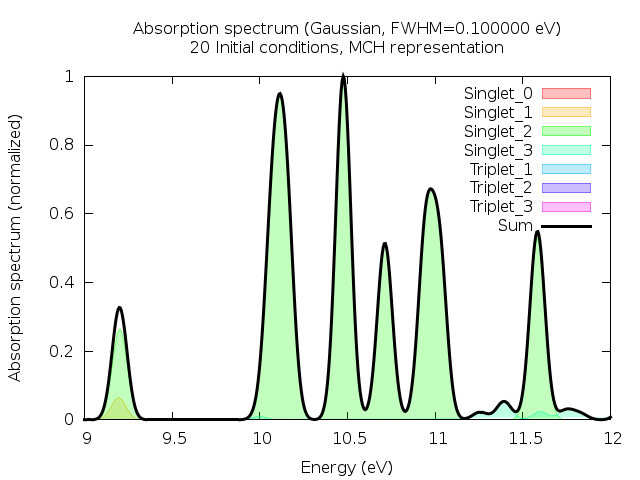
\includegraphics[width=0.75\textwidth]{figures/spectrum.png}
  \caption{Absorption spectrum based on 10 initial conditions (Since there are 20 initial conditions in \ttt{initconds.excited}, the title lists 20 instead of 10).}
  \label{fig:spectrum}
\end{figure}











\clearpage
\section{Setting up dynamics simulations}\label{sec:setup_traj}
\refermanual{m-sec:setup_traj.py}

The last preparatory step towards dynamics simulations consists naturally in setting up the \sharc\ input files and run scripts. 
The interactive script \ttt{setup\_traj.py} takes care of this step. 
Run the script in the directory where the trajectories should be set up. 
For this, create a new directory:
\begin{Verbatim}[commandchars=\\\{\}]
user@host> \textbf{\textcolor{red}{mkdir traj}}
user@host> \textbf{\textcolor{red}{cd traj}}
\end{Verbatim}
Make sure that you have all required files (\ttt{initconds.excited}, \ttt{MOLCAS.template}, \ttt{MOLCAS.RasOrb}) in this directory.
Then start the setup script:
\begin{Verbatim}[commandchars=\\\{\}]
user@host> \textbf{\textcolor{red}{$SHARC/setup_traj.py}}
\end{Verbatim}

\begin{oframed}
\footnotesize\begin{Verbatim}[commandchars=\\\{\}]
  ================================================================================
||                                                                                ||
||                      Setup trajectories for SHARC dynamics                     ||
||                                                                                ||
||                    Author: Sebastian Mai, Philipp Marquetand                   ||
||                                                                                ||
||                                   Version:2.0                                  ||
||                                    01.02.18                                    ||
||                                                                                ||
  ================================================================================


This script automatizes the setup of the input files for SHARC dynamics.
  

  ================================================================================
||                               Initial conditions                               ||
  ================================================================================



This script reads the initial conditions (geometries, velocities, initial excited state)
from the initconds.excited files as provided by excite.py.

Please enter the filename of the initial conditions file.
Initial conditions filename: [initconds.excited] (autocomplete enabled) \textbf{\textcolor{red}{../initconds.excited}}

File ../initconds.excited contains 20 initial conditions.
Number of atoms is 6
Reference energy -94.412945540000 a.u.
Excited states are in MCH representation.


Please enter the number of states as a list of integers
e.g. 3 0 3 for three singlets, zero doublets and three triplets.
Number of states: [4 0 3] \textbf{\textcolor{red}{<ENTER>}}        \textcolor{blue}{# a different number of states than in the}
                                         \textcolor{blue}{# initial calculations could be used in the dynamics}

Number of states: [4, 0, 3]
Total number of states: 13

Do you want all states to be active? [True] \textbf{\textcolor{red}{<ENTER>}}

Do you want to see the content of the initconds file? [True] \textbf{\textcolor{red}{<ENTER>}}
Number of initial conditions in file:          20
Contents of the initconds file:

Legend:
?       Geometry and Velocity
.       not selected
#       selected

State 1:                     \textcolor{blue}{# we only performed 10 calculations, hence the "?"}
             10         20 
              |          | 
 0 | .......... ??????????   \textcolor{blue}{# no initial conditions selected in S0}
State 2:
             10         20 
              |          | 
 0 | .......... ??????????   \textcolor{blue}{# no initial conditions selected in S1}
State 3:
             10         20 
              |          | 
 0 | .######### ??????????   \textcolor{blue}{# initial conditions 2 to 10 are selected}
State 4:
             10         20 
              |          | 
 0 | .......... ??????????   \textcolor{blue}{# no initial conditions selected in S3}
State 5:
             10         20 
              |          | 
 0 | .......... ??????????   \textcolor{blue}{# no initial conditions selected in T1}
State 6:
             10         20 
              |          | 
 0 | .......... ??????????   \textcolor{blue}{# no initial conditions selected in T2}
State 7:
             10         20 
              |          | 
 0 | .......... ??????????   \textcolor{blue}{# no initial conditions selected in T3}
State 8:
             10         20 
              |          | 
 0 | .......... ?????????? 
State 9:
             10         20 
              |          | 
 0 | .......... ?????????? 
State 10:
             10         20 
              |          | 
 0 | .......... ?????????? 
State 11:
             10         20 
              |          | 
 0 | .......... ?????????? 
State 12:
             10         20 
              |          | 
 0 | .......... ?????????? 
State 13:
             10         20 
              |          | 
 0 | .......... ?????????? 
Number of excited states and selections:
State    #InitCalc       #Selected
    1           10               0
    2           10               0
    3           10               9  \textcolor{blue}{# we can setup 9 trajectories starting in state 3 (S2)}
    4           10               0
    5           10               0
    6           10               0
    7           10               0
    8           10               0
    9           10               0
   10           10               0
   11           10               0
   12           10               0
   13           10               0

Please enter a list specifying for which excited states trajectories should be set-up
e.g. 6 10 11 to select states 6, 10, and 11.
States to setup the dynamics: [3] (range comprehension enabled) \textbf{\textcolor{red}{<ENTER>}}

There can be 9 trajectories set up.

Please enter the index of the first initial condition in the initconds file to be setup.
Starting index: [1] \textbf{\textcolor{red}{<ENTER>}}

There can be 9 trajectories set up, starting in 1 states.

Please enter the total number of trajectories to setup.
Number of trajectories: [9] \textbf{\textcolor{red}{<ENTER>}}

Please enter a random number generator seed (type "!" to initialize the RNG from the system time).
RNG Seed:  [!] \textbf{\textcolor{red}{1234}}


  ================================================================================
||                     Choose the quantum chemistry interface                     ||
  ================================================================================


Please specify the quantum chemistry interface (enter any of the following numbers):
1       MOLPRO (only CASSCF)
2       COLUMBUS (CASSCF, RASSCF and MRCISD), using SEWARD integrals
3       Analytical PESs
4       MOLCAS (CASSCF, CASPT2, MS-CASPT2)
5       ADF (DFT, TD-DFT)
6       TURBOMOLE (ricc2 with CC2 and ADC(2))
7       LVC Hamiltonian
8       GAUSSIAN (DFT, TD-DFT)

Interface number: \textbf{\textcolor{red}{4}}

  ================================================================================
||                        Surface Hopping dynamics settings                       ||
  ================================================================================


-----------------------Simulation time----------------------

Please enter the total simulation time.
Simulation time (fs): [1000.0] \textbf{\textcolor{red}{100}}

Please enter the simulation timestep (0.5 fs recommended).
Simulation timestep (fs): [0.5] \textbf{\textcolor{red}{<ENTER>}}

Simulation will have 201 timesteps.

Please enter the number of substeps for propagation (25 recommended).
Nsubsteps: [25] \textbf{\textcolor{red}{<ENTER>}}

The trajectories can be prematurely terminated after they run for a certain time in the lowest state. 
Do you want to prematurely terminate trajectories? [False] \textbf{\textcolor{red}{<ENTER>}}


----------------------Dynamics settings---------------------

Do you want to perform the dynamics in the diagonal representation (SHARC dynamics) 
or in the MCH representation (regular surface hopping)?
SHARC dynamics? [True] \textbf{\textcolor{red}{<ENTER>}}
Do you want to include spin-orbit couplings in the dynamics?

Spin-Orbit calculation? [True] \textbf{\textcolor{red}{<ENTER>}}
Will calculate spin-orbit matrix.


Please choose the quantities to describe non-adiabatic effects between the states:
1       DDT     =  < a|d/dt|b >        Hammes-Schiffer-Tully scheme   (not available)
2       DDR     =  < a|d/dR|b >        Original Tully scheme          (not available)
3       overlap = < a(t0)|b(t) >       Local Diabatization scheme     
Coupling number: [3] \textbf{\textcolor{red}{<ENTER>}}

For SHARC dynamics, the evaluation of the mixed gradients necessitates to calculate 
non-adiabatic coupling vectors (Extra computational cost).
... but interface cannot provide non-adiabatic coupling vectors, turning option off.

During a surface hop, the kinetic energy has to be modified in order to conserve total energy. 
There are several options to that:
1       Do not conserve total energy. Hops are never frustrated.
2       Adjust kinetic energy by rescaling the velocity vectors. Often sufficient.
3       Adjust kinetic energy only with the component of the velocity vector along 
        the non-adiabatic coupling vector.        (not possible)
EkinCorrect: [2] \textbf{\textcolor{red}{<ENTER>}}

If a surface hop is refused (frustrated) due to insufficient energy, the velocity can either be 
left unchanged or reflected:
1       Do not reflect at a frustrated hop.
2       Reflect the full velocity vector.
3       Reflect only the component of the velocity vector along the non-adiabatic coupling vector.
        (not possible)
Reflect frustrated: [1] \textbf{\textcolor{red}{<ENTER>}}

Please choose a decoherence correction for the diagonal states:
1       No decoherence correction.
2       Energy-based decoherence scheme (Granucci, Persico, Zoccante).
3       Augmented fewest-switching surface hopping (Jain, Alguire, Subotnik).
Decoherence scheme: [2] \textbf{\textcolor{red}{<ENTER>}}

Please choose a surface hopping scheme for the diagonal states:
1       Surface hops off.
2       Standard SHARC surface hopping probabilities (Mai, Marquetand, Gonzalez).
3       Global flux surface hopping probabilities (Wang, Trivedi, Prezhdo).
Hopping scheme: [2] \textbf{\textcolor{red}{<ENTER>}}

Do you want to scale the energies and gradients?
Scaling? [False] \textbf{\textcolor{red}{<ENTER>}}

Do you want to damp the dynamics (Kinetic energy is reduced at each timestep by a factor)?
Damping? [False] \textbf{\textcolor{red}{<ENTER>}}

Do you want to use an atom mask for velocity rescaling or decoherence?
Atom masking? [False] \textbf{\textcolor{red}{<ENTER>}}

---------------Selection of Gradients and NACs--------------

In order to speed up calculations, SHARC is able to select which gradients and NAC vectors it has to 
calculate at a certain timestep. The selection is based on the energy difference between the state 
under consideration and the classical occupied state.

Select gradients? [False] \textbf{\textcolor{red}{yes}}    \textcolor{blue}{# this strongly speeds up the calculations}

Please enter the energy difference threshold for the selection of gradients and non-adiabatic 
couplings (in eV). (0.5 eV recommended, or even larger if SOC is strong in this system.)
Selection threshold (eV): [0.5] \textbf{\textcolor{red}{0.1}}


-------------------------Laser file-------------------------

Do you want to include a laser field in the simulation? [False] \textbf{\textcolor{red}{<ENTER>}}

  ================================================================================
||                             MOLCAS Interface setup                             ||
  ================================================================================


-----------------------Path to MOLCAS-----------------------

Please specify path to MOLCAS directory (SHELL variables and ~ can be used, 
will be expanded when interface is started).

Path to MOLCAS: [$MOLCAS/] (autocomplete enabled) \textbf{\textcolor{red}{<ENTER>}}

----------------------Scratch directory---------------------

Please specify an appropriate scratch directory. This will be used to temporally 
store the integrals. The scratch directory will be deleted after the calculation. 
Remember that this script cannot check whether the path is valid, since you may 
run the calculations on a different machine. The path will not be expanded by this script.
Path to scratch directory: (autocomplete enabled) \textbf{\textcolor{red}{$TMPDIR/Tutorial/Traj_WORK/}}

-----------------MOLCAS input template file-----------------

Please specify the path to the MOLcas.template file. This file must contain the following settings:

basis <Basis set>
ras2 <Number of active orbitals>
nactel <Number of active electrons>
inactive <Number of doubly occupied orbitals>
roots <Number of roots for state-averaging>

The MOLCAS interface will generate the appropriate MOLCAS input automatically.

Template filename: (autocomplete enabled) \textbf{\textcolor{red}{../MOLCAS.template}}

---------------Initial wavefunction: MO Guess---------------

Please specify the path to a MOLCAS JobIph file containing suitable starting MOs for the CASSCF 
calculation. Please note that this script cannot check whether the wavefunction file and the 
Input template are consistent!

Do you have initial wavefunction files for Singlet, Triplet? [True] \textbf{\textcolor{red}{<ENTER>}}
JobIph files (1) or RasOrb files (2)? \textbf{\textcolor{red}{2}}
Initial wavefunction file for Singlets: [MOLCAS.1.RasOrb.init] (autocomplete enabled) \textbf{\textcolor{red}{../MOLCAS.RasOrb}}
Initial wavefunction file for Triplets: [MOLCAS.3.RasOrb.init] (autocomplete enabled) \textbf{\textcolor{red}{../MOLCAS.RasOrb}}
-------------------MOLCAS Ressource usage-------------------

Please specify the amount of memory available to MOLCAS (in MB). For calculations including moderately-
sized CASSCF calculations and less than 150 basis functions, around 2000 MB should be sufficient.

MOLCAS memory: \textbf{\textcolor{red}{500}}
Please specify the number of CPUs to be used by EACH calculation.

Number of CPUs: \textbf{\textcolor{red}{1}}

  ================================================================================
||                           Content of output.dat files                          ||
  ================================================================================


Do you want to write the gradients to the output.dat file ?
Write gradients? [False] \textbf{\textcolor{red}{<ENTER>}}

Do you want to write the non-adiabatic couplings (NACs) to the output.dat file ?
Write NACs? [False] \textbf{\textcolor{red}{<ENTER>}}

Do you want to write property matrices to the output.dat file  (e.g., Dyson norms)?
Write property matrices? [False] \textbf{\textcolor{red}{<ENTER>}}

Do you want to write property vectors to the output.dat file  (e.g., TheoDORE results)?
Write property vectors? [False] \textbf{\textcolor{red}{<ENTER>}}

Do you want to write the overlap matrix to the output.dat file ?
Write overlap matrix? [True] \textbf{\textcolor{red}{<ENTER>}}


  ================================================================================
||                                 Run mode setup                                 ||
  ================================================================================


-------------------------Run script-------------------------

This script can generate the run scripts for each trajectory in two modes:

  - In the first mode, the calculation is run in subdirectories of the current directory.

  - In the second mode, the input files are transferred to another directory (e.g. a local scratch 
  directory), the calculation is run there, results are copied back and the temporary directory is 
  deleted. Note that this temporary directory is not the same as the scratchdir employed by the interfaces.

Note that in any case this script will setup the input subdirectories in the current working directory.

Do you want to use mode 1 
(actually perform the calculations in subdirectories of: 
/user/mai/Documents/NewSHARC/SHARC_2.0/TUTORIAL/2_full/Tutorial/traj)

Calculate here? [True] \textbf{\textcolor{red}{<ENTER>}}

----------------------Submission script---------------------

During the setup, a script for running all initial conditions sequentially in batch mode is generated. 
Additionally, a queue submission script can be generated for all initial conditions.

Generate submission script? [False] \textbf{\textcolor{red}{<ENTER>}}


#########################Full input#########################

molcas                     $MOLCAS/
soc                        True
ntraj                      9
ninit                      20
molcas.guess               \{1: '../MOLCAS.RasOrb', 3: '../MOLCAS.RasOrb'\}
write_NAC                  False
write_property1d           False
dipolegrad                 False
states                     [4, 0, 3]
molcas.jobiph_or_rasorb    2
kill                       False
qsub                       False
nstates                    13
show_content               True
molcas.ncpu                1
eharm                      0.0
n_issel                    [0, 0, 9, 0, 0, 0, 0, 0, 0, 0, 0, 0, 0]
nsubstep                   25
scratchdir                 $TMPDIR/Tutorial/Traj_WORK/
diag                       False
actstates                  [4, 0, 3]
ekincorrect                2
atommaskarray              []
needed                     []
eselect                    0.1
eref                       -94.41294554
damping                    False
molcas.mem                 500
firstindex                 1
cwd                        /user/mai/Documents/NewSHARC/SHARC_2.0/TUTORIAL/2_full/Tutorial/traj
write_property2d           False
surf                       diagonal
initf                      <open file '../initconds.excited', mode 'r' at 0x1714c90>
molcas.template            ../MOLCAS.template
dtstep                     0.5
repr                       MCH
phases_from_interface      False
reflect                    1
ion                        False
statemap                   \{1: [1, 1, 0.0], 
                            2: [1, 2, 0.0], 
                            3: [1, 3, 0.0], 
                            4: [1, 4, 0.0], 
                            5: [3, 1, -1.0], 
                            6: [3, 2, -1.0], 
                            7: [3, 3, -1.0], 
                            8: [3, 1, 0.0], 
                            9: [3, 2, 0.0], 
                            10: [3, 3, 0.0], 
                            11: [3, 1, 1.0], 
                            12: [3, 2, 1.0], 
                            13: [3, 3, 1.0]\}
here                       True
interface                  4
write_overlap              True
scaling                    False
laser                      False
coupling                   3
hopping                    sharc
sel_g                      True
tmax                       100.0
write_grad                 False
copydir                    /user/mai/Documents/NewSHARC/SHARC_2.0/TUTORIAL/2_full/Tutorial/traj
sel_t                      False
setupstates                set([3])
printlevel                 2
natom                      6
gradcorrect                False
decoherence                ['edc', '0.1']
isactive                   [True, True, True, True, True, True, True, True, True, True, True, True, True]

Do you want to setup the specified calculations? [True] \textbf{\textcolor{red}{<ENTER>}}


  ================================================================================
||                            Setting up directories...                           ||
  ================================================================================


Progress: [==================================================] 100%

9 trajectories setup, last initial condition was 10 in state 3.
\end{Verbatim}
\end{oframed}

\normalsize

The script creates for each of the initial states (``States to setup the dynamics'') a directory called \ttt{<Mult>\_<Num>}, e.g., \ttt{Singlet\_2/}, which contains the input for all trajectories starting in that state. 
Each of these directories contains subdirectories named \ttt{TRAJ\_00001/}, \ttt{TRAJ\_00002/}, etc. 
Note that these numbers are not consecutive: if an initial condition has not been selected, the number will be missing.
Each subdirectory contains the \sharc\ input (consisting of the files \ttt{input}, \ttt{geom}, and \ttt{veloc}), the directories \ttt{QM/} and \ttt{restart/}, and the run script for the trajectory, \ttt{run.sh}.

For the purposes of the tutorial it is sufficient to only calculate one trajectory. Change to the subdirectory of one of the trajectories and execute it.
\begin{Verbatim}[commandchars=\\\{\}]
user@host> \textbf{\textcolor{red}{cd Singlet_2/TRAJ_00002}}
user@host> \textbf{\textcolor{red}{sh run.sh&}}
user@host> \textbf{\textcolor{red}{tailf output.lis}}
\end{Verbatim}
While the trajectory is running, you can watch its progress in the file \ttt{output.lis} (short output listing). For each timestep, it contains the currently occupied diagonal state (and approximate MCH state), the kinetic, potential and total energy, the RMS gradient, the state dipole and spin expectation values of the currently occupied diagonal state and the time needed for this step. Surface hopping events are also mentioned in this file.

Besides the \ttt{output.lis} file, \sharc\ creates the files \ttt{output.log}, \ttt{output.xyz} and \ttt{output.dat}. 
The file
\ttt{output.log} contains mainly parsing information of the input file parsing and a list of internal steps of the dynamics simulation. 
With sufficiently high \ttt{printlevel} in the \sharc\ input file, the log file may also contain debug information in various detail, but with the default setting, no relevant information is printed.
The file \ttt{output.dat} contains for each timestep the most important matrices and vectors. 
This information can be used to calculate the excited-state energies, populations, hopping probabilities and a large number of expectation values. 
See below for the usage of \ttt{data\_extractor.x} and \ttt{make\_gnuplot.py}, which can be used for plotting the mentioned quantities.
Finally, \ttt{output.xyz} contains the cartesian coordinates of all atoms for each timestep. 
This file can be opened with any program capable of processing xyz files, like \textsc{Molden}, \textsc{Molekel} and \textsc{Gabedit}. 
Additionally, the geometries can be analyzed with the programs \ttt{geo.py}, which is a command line tool to extract internal coordinates from such an xyz file, \ttt{trajana\_nma.py}, and \ttt{trajana\_essdyn.py}.



% ===========================================================================================================================
% ===========================================================================================================================
% ===========================================================================================================================

\clearpage
\section{Analyzing a single trajectory}

We will first discuss the analysis of a single trajectory based on the output files. 
Later (section~\ref{sec:analyze_ensemble}) we will also analyze ensemble properties. 

If you are not in the directory for the trajectory \ttt{TRAJ\_00002/}, change to this directory:
\begin{Verbatim}[commandchars=\\\{\}]
user@host> \textbf{\textcolor{red}{cd Singlet_2/TRAJ_00002}}
\end{Verbatim}


% ======================================================================================================

\subsection{Data extraction and plotting}
\refermanual{m-sec:data_extractor.x}
\refermanual{m-sec:make_gnuscript.py}

The file \ttt{output.dat} contains the Hamiltonian, transformation matrix, dipole matrices, coefficients, hopping probabilities, kinetic energy and random number from the surface hopping procedure in a compressed form. The program \ttt{data\_extractor.x} can be used to generate data tables, which can then be plotted.
\begin{Verbatim}[commandchars=\\\{\}]
user@host> \textbf{\textcolor{red}{$SHARC/data_extractor.x output.dat}}
\end{Verbatim}
The program creates a subdirectory called \ttt{output\_data/}. With the default settings, the following files will be created:
\begin{itemize}
  \item \ttt{coeff\_diab.out} contains the coefficients in the diabatic representation (only approximate).
  \item \ttt{coeff\_diag.out} contains the coefficients in the diagonal representation.
  \item \ttt{coeff\_MCH.out} contains the coefficients in the MCH representation.
  \item \ttt{energy.out} contains kinetic, current potential, total and potential energy of all excited states.
  \item \ttt{fosc.out} contains the oscillator strengths of the current state and all excited states.
  \item \ttt{spin.out} contains the total spin expectation values of the current state and all excited states.
  \item \ttt{prob.out} contains the surface hopping random number and the hopping probabilities in the diagonal representation.
  \item \ttt{expec.out} contains the content of \ttt{energy.out}, \ttt{fosc.out} and \ttt{spin.out} in one file (for plotting).
  \item \ttt{expec\_MCH.out} is analogue to \ttt{expec.out}, except all data is given in the MCH representation.
\end{itemize}

In order to plot the content of these files in an efficient manner, \ttt{gnuplot} can be used. Use
\begin{Verbatim}[commandchars=\\\{\}]
user@host> \textbf{\textcolor{red}{$SHARC/make_gnuscript.py  4  0  3 > plot.gp}}
\end{Verbatim}
to create a \ttt{gnuplot} script with the correct state numbering and labeling. Execute
\begin{Verbatim}[commandchars=\\\{\}]
user@host> \textbf{\textcolor{red}{gnuplot plot.gp}}
\end{Verbatim}
to plot energies, populations and hopping probabilities (Use \textcolor{red}{\ttt{<ENTER>}} to continue with the next plot). In figures~\ref{fig:en}, \ref{fig:cMCH}, \ref{fig:cDIAG} and~\ref{fig:prob} the output for trajectory \ttt{TRAJ\_00002/} for the first 100~fs is given.


\begin{figure}[tb]
  \centering
  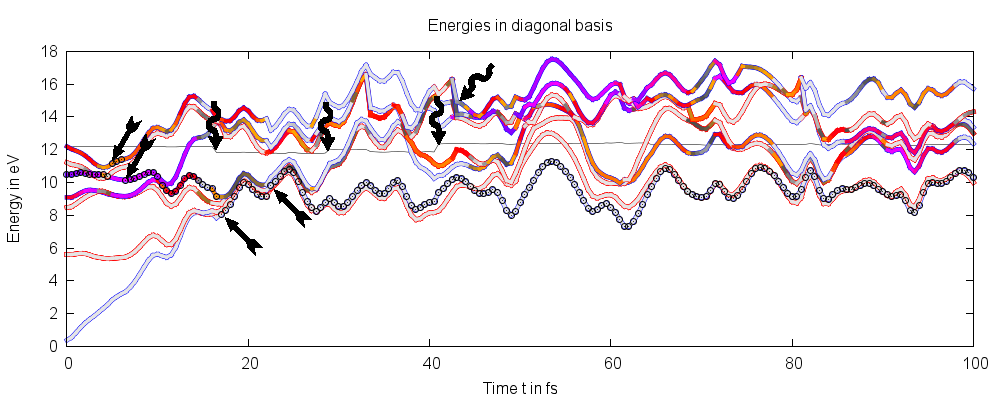
\includegraphics[width=\textwidth]{figures/energy.png}
  \caption{Plot of the potential energies for trajectory \ttt{TRAJ\_00002/} with 4 singlet and 3 triplet states. Straight arrows indicate hopping events discussed in the text, wiggly arrows indicate problems with energy conservation/continuity. }
  \label{fig:en}
\end{figure}
\begin{figure}[p]
  \centering
  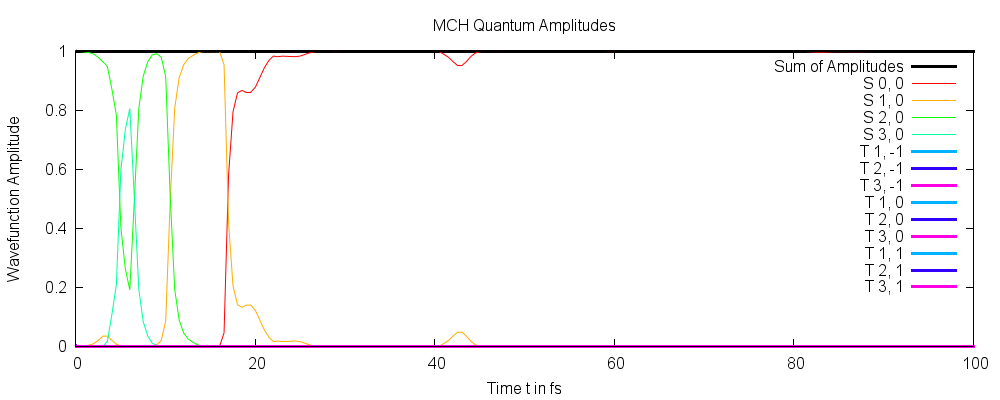
\includegraphics[width=0.95\textwidth]{figures/coeff_MCH.png}
  \caption{Plot of the excited-state populations in the MCH representation.}
  \label{fig:cMCH}
\end{figure}
\begin{figure}[p]
  \centering
  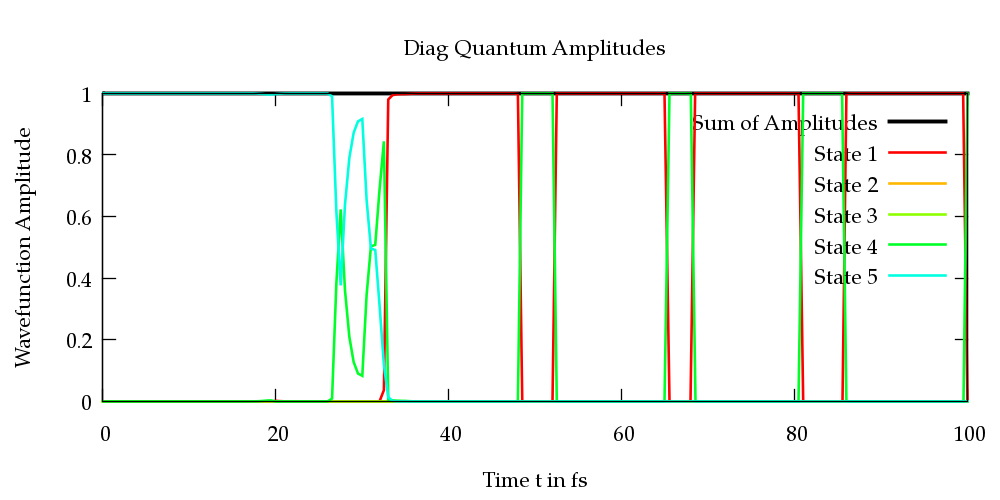
\includegraphics[width=0.95\textwidth]{figures/coeff_diag.png}
  \caption{Plot of the excited-state populations in the diagonal representation.}
  \label{fig:cDIAG}
\end{figure}
\begin{figure}[p]
  \centering
  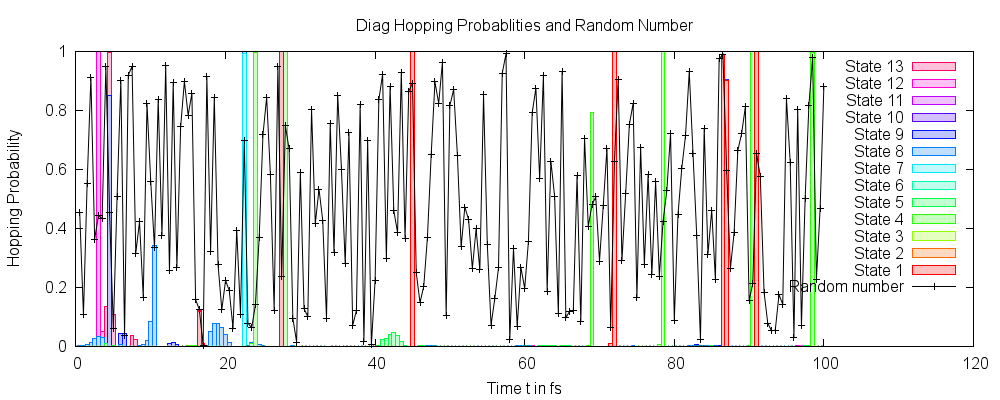
\includegraphics[width=0.95\textwidth]{figures/prob.png}
  \caption{Plot of the hopping probabilities in the diagonal representation. Additionally, the random number for the surface hopping procedure is given.}
  \label{fig:prob}
\end{figure}

\paragraph{Discussion of Figure~\ref{fig:en}}

In figure~\ref{fig:en}, the potential energies of all states included in the dynamics depending on time is given. 
The total energy is given by the thin black line (around 12~eV) and the currently occupied state is marked with black circles. 
Each state is represented by a line that is colored in two ways, with an inner core color and an outer colored contour.
The inner color encodes the oscillator strength of the state at each instant of time. 
Dark states are \textcolor{black!20}{light grey}, while brighter states are given in \textcolor{black!40}{grey}, \textcolor{black!70}{dark grey}, \textcolor{red!60!green}{orange}, \textcolor{red}{red}, \textcolor{red!50!blue}{magenta} or \textcolor{blue}{blue}, in order of increasing oscillator strength. 
The outer color encodes the total spin expectation value. 
Singlets are \textcolor{blue}{blue}, triplets \textcolor{red}{red} and states with mixed singlet-triplet character are \textcolor{green!90!black}{green}. 
Since in the methaniminium cation spin-orbit coupling is negligible, in the figure only blue and red contours are visible.

In the figure, the trajectory starts in the very bright singlet state slightly above 10~eV (the $S_3$).
The ground state (grey/blue line), the $T_1$ and $T_2$ (grey/red lines), and the $S_1$ (red/blue line) are at lower energies, whereas the $T_3$ (grey/red line) and the $S_4$ (red/blue line) are at higher energies.
All important nonadiabatic events occur within the first 25~fs.
In the figure, four hopping events are marked with straight arrows (at 5.0~fs, 6.5~fs, 17.0~fs, and 22.5~fs; note that these are not the only hopping events in the figure).
It can be seen that the trajectory briefly switches to the $S_4$ state but quickly returns to $S_3$.
Subsequently, it changes to $S_1$ and then to $S_0$ (at 17.0~fs).
The hop at 22.5~fs is due to a crossing of the $S_0$ with the $T_1$, and since the $T_1$ is not populated, the trajectory hops to stay in the singlet state.
For the remainder of the simulation time, the trajectory stays in $S_0$, occasionally performing a hop at $S_0/T_1$ crossings.
The very high potential energy indicates that the trajectory did not simply return to the ground state equilibrium geometry.

In the figure, four wiggly arrows indicate possible problems in the trajectory.
Three of these arrows (at 17.0~fs, 29.0~fs, and 41.0~fs) point to time steps where the total energy was not well conserved.
In general, this can have different reasons (e.g., wrong gradients, too large time steps, convergence problems), but here all three cases are due to abrupt changes in the active space because the highest singlet state crossed with another state.
Often, this problem can be circumvented by a good choice of the active space and the number of roots for state averaging.
The fourth wiggly arrow (at 43.0~fs) points to a time step where the same problem happens to the triplet states; note how the $T_3$ energy suddenly changes.
Since in \textsc{Molcas} each multiplicity uses its own active space, this does not affect the singlet states and thus the trajectory.
However, in systems with larger spin-orbit couplings, such state switches might lead to unphysical population transfer to the triplet states.

Ultimately, the user is responsible to check the trajectories for such problematic time steps.
For the purposes of the tutorial, we will ignore these energy conservation problems.
Note that this trajectory checking can also be carried out while the trajectories are still running; if a problematic trajectory is encountered, it can be terminated gracefully by creating an empty file called \ttt{STOP} in the run directory of that trajectory.

\paragraph{Discussion of Figure~\ref{fig:cMCH}}

In figure~\ref{fig:cMCH}, the MCH populations are given depending on time. The system starts with 100\% of the population in the $S_2$. 
Around 5~fs, part of the population is briefly transferred to the $S_3$.
Then, at 10~fs population flows to the $S_1$, and at 17~fs to the $S_0$, where it stays for the remainder of the simulation.
The population of the triplet states is approximately zero for all time steps, as was expected for this system.

It is instructive to observe the correlation between the population transfers in figure~\ref{fig:cMCH} with the hopping events in figure~\ref{fig:en}.


\paragraph{Discussion of Figure~\ref{fig:cDIAG}}

In figure~\ref{fig:cDIAG}, the diagonal populations are given depending on time. 
The difference between the MCH and diagonal populations is due to the fact that the diagonal states are strictly ordered according to energy.
This can be seen best in the second half of the figure, where population is occasionally exchanged (with 100\% efficiency) between state 1 and state 4.
These population transfers happen where the $S_0$ and $T_1$ states cross (e.g., before the crossing the $S_0$ is lower than $T_1$ and hence $S_0$ is state 1. After the crossing, $S_0$ becomes state 4, and the population is transferred to state 4 to conserve the spin multiplicity of the total wave function).

Note that in more complicated cases, the diagonal populations are of little use for interpretation purposes, so that most users will prefer to analyze the MCH populations.


\paragraph{Discussion of Figure~\ref{fig:prob}}

Figure~\ref{fig:prob} shows the surface hopping probabilities and the corresponding random numbers depending on time.
In a nutshell, a surface hop happens whenever the random number lies within one of the colored bars. 
The color of the bar corresponds to the state into which the trajectory will hop. 
In the diagram, there are several hopping probabilities close to unity. 
This corresponds to the near-complete population transfer during the crossing of the singlet and triplet states. 



% ======================================================================================================

\clearpage
\subsection{Analyzing internal coordinates}
\refermanual{m-sec:geo.py}
\refermanual{m-met:geo}

The file \ttt{output.xyz} contains the cartesian coordinates of all timesteps. 
Oftentimes, one is interested in the variation of certain internal coordinates (like bond lengths, angles, etc.) during the dynamics. 
The \sharc\ tool \ttt{geo.py} can quickly calculate these values. 
Invoke the program and enter the internal coordinate specifications:
\begin{Verbatim}[commandchars=\\\{\}]
user@host> \textbf{\textcolor{red}{$SHARC/geo.py -g output.xyz -t 0.5}}
\end{Verbatim}

\begin{oframed}
\footnotesize\begin{Verbatim}[commandchars=\\\{\}]
Enter the internal coordinate specifications:
\textcolor{red}{r 1 2}
\textcolor{red}{d 3 1 2 4}
\textcolor{red}{end}
Number of internal coordinate requests:   2
Number of geometries:    200
FINISHED!
\end{Verbatim}
\end{oframed}

\normalsize
The \ttt{-g} option specifies the filename of the input xyz geometry file, while the \ttt{-t} option specifies the timestep. \ttt{geo.py} writes the results to standard out, so redirect the output to some file:
\begin{Verbatim}[commandchars=\\\{\}]
user@host> \textbf{\textcolor{red}{$SHARC/geo.py -g output.xyz -t 0.5 > Geo.out}}
\end{Verbatim}
The file \ttt{Geo.out} contains a table with the specified internal coordinates:
\begin{oframed}
\footnotesize\begin{Verbatim}[commandchars=\\\{\}]
#                  1|                   2|                   3|
#               time|             r  1  2|       d  6  1  2  5|
              0.0000               1.3024              16.2632 
              0.5000               1.3135              18.5857 
              1.0000               1.3293              20.6828 
                   \vdots                    \vdots                    \vdots
\end{Verbatim}
\end{oframed}

Use \textsc{Gnuplot} to plot this table. 
\begin{Verbatim}[commandchars=\\\{\}]
user@host> \textcolor{red}{gnuplot}
\end{Verbatim}
The file \ttt{Geo.out} contains a table with the specified internal coordinates:
\begin{oframed}
\footnotesize\begin{Verbatim}[commandchars=\\\{\}]
gnuplot> \textcolor{red}{p "Geo.out" u 1:2 w l}     \textcolor{blue}{# Plot column 2 versus 1}
gnuplot> \textcolor{red}{p "Geo.out" u 1:3 w l}     \textcolor{blue}{# Plot column 3 versus 1}
\end{Verbatim}
\end{oframed}

\normalsize
The results are shown in figures \ref{fig:cc} and \ref{fig:dih}.

\paragraph{Discussion of the internal coordinates} 

In figures~\ref{fig:cc} the \ce{C=N} bond length is plotted over time. It can be easily seen that after excitation to the $\pi\pi^*$ state, the \ce{C=N} bond stretches strongly and reaches more than 3\,\AA after 100~fs.
This is a clear sign that the \ce{CH2NH2+} molecule is dissociating in this trajectory.

In figure~\ref{fig:dih}, the dihedral angle \ce{H-C=N-H} is plotted in degrees (confined to the interval $[-180^\circ,180^\circ]$). 
It can be seen that after excitation the molecule undergoes torsion around the central bond.

\begin{figure}[htb]
  \centering
  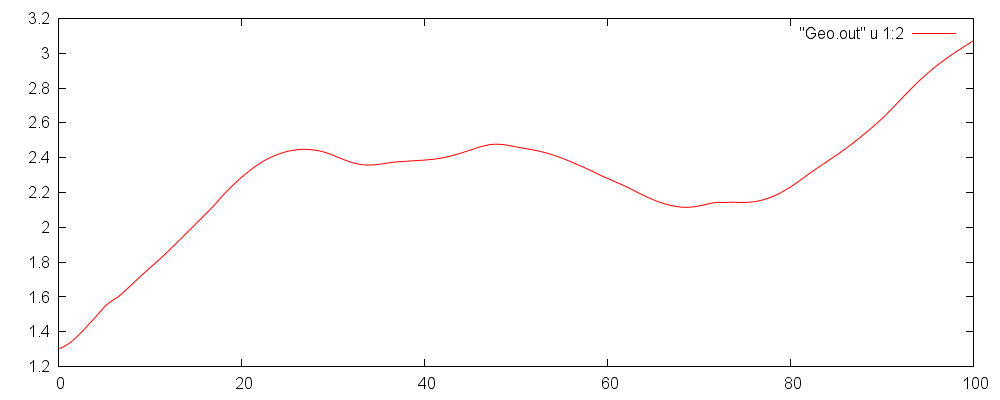
\includegraphics[width=\textwidth]{figures/CC.png}
  \caption{Value of the \ce{C=C} bond length during the simulation.}
  \label{fig:cc}
\end{figure}
\begin{figure}[htb]
  \centering
  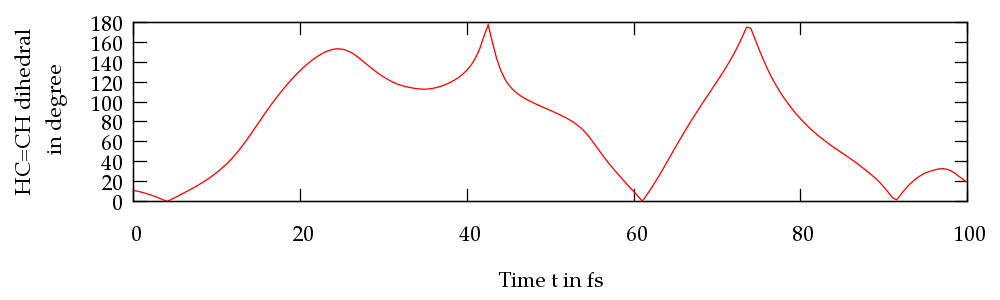
\includegraphics[width=\textwidth]{figures/dih.png}
  \caption{Value of one of the \ce{H-C=C-H} dihedrals during the simulation.}
  \label{fig:dih}
\end{figure}

In order to confirm these findings, it is recommended that you load \ttt{output.xyz} into \textsc{Molden} (or another program) to watch the trajectory as a movie.







% ======================================================================================================

\clearpage
\section{Analyzing the Ensemble}\label{sec:analyze_ensemble}

For these analysis the tutorial assumes that you ran all nine trajectories (\ttt{TRAJ\_00002/} to \ttt{TRAJ\_00009/}).

\subsection{Ensemble Diagnostics}
\refermanual{m-sec:diagnostics.py}

It is always a good idea to inspect the trajectories before starting with the ensemble analysis, because within the large ensemble it might not be possible to spot problems of a single trajectory.
There are two ways to inspect the trajectories---either manually checking them as described above, or the ensemble diagnostics tool, \ttt{diagnostics.py}.
This script performs a number of sanity checks for all trajectories (file existence, consistency, energy conservation, intruder states), and allows automatically marking problematic trajectories to exclude them from the analysis steps.

If you are still in the directory \ttt{TRAJ\_00002/}, go back to the root directory of the ensemble.
Then, execute \ttt{diagnostics.py}:
\begin{Verbatim}[commandchars=\\\{\}]
user@host> \textbf{\textcolor{red}{cd ../..}}
user@host> \textbf{\textcolor{red}{$SHARC/diagnostics.py}}
\end{Verbatim}


\begin{oframed}
\footnotesize\begin{Verbatim}[commandchars=\\\{\}]
  ================================================================================
||                                                                                ||
||              Diagnostic tool for trajectories from SHARC dynamics              ||
||                                                                                ||
||                              Author: Sebastian Mai                             ||
||                                                                                ||
||                                   Version:2.0                                  ||
||                                    01.02.18                                    ||
||                                                                                ||
  ================================================================================


This script reads output.dat files from SHARC trajectories and checks:
* missing files
* normal termination
* total energy conservation
* total population conservation
* discontinuities in potential and kinetic energy
  
--------------------Paths to trajectories-------------------

Please enter the paths to all directories containing the "TRAJ_0XXXX" directories.
E.g. Sing_2/ and Sing_3/. 
Please enter one path at a time, and type "end" to finish the list.
Path:  [end] (autocomplete enabled) \textbf{\textcolor{red}{Singlet_2/}}
['TRAJ_00005', 'TRAJ_00004', 'TRAJ_00008', 'TRAJ_00009', 'TRAJ_00002', 
'TRAJ_00006', 'TRAJ_00010', 'TRAJ_00007', 'TRAJ_00003']
Found 9 subdirectories in total.

Path:  [end] (autocomplete enabled) \textbf{\textcolor{red}{<ENTER>}}

{'paths': ['Singlet_2/']}
Total number of subdirectories: 9

['nstates', '4', '0', '3']
---------------------Diagnostic settings--------------------

Please, adjust the diagnostic settings according to your preferences.
You can use the following commands:
show            Prints the current settings
help            Prints explanations for the keys
end             Save and continue
<key> <value>   Adjust setting.

Current settings:
        missing_output : True
       missing_restart : True
    normal_termination : True
           etot_window : 0.2
             etot_step : 0.1
             epot_step : 0.7
             ekin_step : 0.7
            pop_window : 1e-07
            hop_energy : 1.0
             intruders : True

?  [end] \textbf{\textcolor{red}{<ENTER>}}
#########################Full input#########################

paths                      ['Singlet_2/']
settings                   \{'missing_restart': True, 
                            'etot_step': 0.1, 
                            'hop_energy': 1.0, 
                            'epot_step': 0.7, 
                            'ekin_step': 0.7, 
                            'intruders': True, 
                            'pop_window': 1e-07, 
                            'missing_output': True, 
                            'normal_termination': True, 
                            'etot_window': 0.2\}

Do you want to do the specified analysis? [True] \textbf{\textcolor{red}{<ENTER>}}

Checking the directories...
~~~~~~~~~~~~~~~~~~~~~~~~~~~~~ Singlet_2/TRAJ_00002 ~~~~~~~~~~~~~~~~~~~~~~~~~~~~~

    Output files:     .lis .. .log .. .dat .. .xyz .. OK
    Restart files:    ctrl .. traj .. restart/ ..     OK
    Progress:         [=========================]     100.0 of 100.0 fs
    Status:                                           FINISHED
    Energy:           Large dE during hop             at 6.50 fs      \textcolor{blue}{# a hop over >1eV might be suspicious}
    Population:                                       OK
    Intruder states:                                  OK



~~~~~~~~~~~~~~~~~~~~~~~~~~~~~ Singlet_2/TRAJ_00003 ~~~~~~~~~~~~~~~~~~~~~~~~~~~~~

    Output files:     .lis .. .log .. .dat .. .xyz .. OK
    Restart files:    ctrl .. traj .. restart/ ..     OK
    Progress:         [=========================]     100.0 of 100.0 fs
    Status:                                           FINISHED
    Energy:           Large dE during hop             at 11.50 fs
    Population:                                       OK
    Intruder states:                                  OK



~~~~~~~~~~~~~~~~~~~~~~~~~~~~~ Singlet_2/TRAJ_00004 ~~~~~~~~~~~~~~~~~~~~~~~~~~~~~

    Output files:     .lis .. .log .. .dat .. .xyz .. OK
    Restart files:    ctrl .. traj .. restart/ ..     OK
    Progress:         [=========================]     100.0 of 100.0 fs
    Status:                                           FINISHED
    Energy:           Large step in Epot              at 13.50 fs      \textcolor{blue}{# time step might be too long here}
    Population:                                       OK
    Intruder states:                                  OK



~~~~~~~~~~~~~~~~~~~~~~~~~~~~~ Singlet_2/TRAJ_00005 ~~~~~~~~~~~~~~~~~~~~~~~~~~~~~

    Output files:     .lis .. .log .. .dat .. .xyz .. OK
    Restart files:    ctrl .. traj .. restart/ ..     OK
    Progress:         [=========================]     100.0 of 100.0 fs
    Status:                                           FINISHED
    Energy:           Large step in Etot              at 29.00 fs    \textcolor{blue}{# problem due to active space switch}
    Population:                                       OK
    Intruder states:                                  OK



~~~~~~~~~~~~~~~~~~~~~~~~~~~~~ Singlet_2/TRAJ_00006 ~~~~~~~~~~~~~~~~~~~~~~~~~~~~~

    Output files:     .lis .. .log .. .dat .. .xyz .. OK
    Restart files:    ctrl .. traj .. restart/ ..     OK
    Progress:         [=========================]     100.0 of 100.0 fs
    Status:                                           FINISHED
    Energy:           Large step in Etot              at 3.50 fs
    Population:                                       OK
    Intruder states:                                  OK



~~~~~~~~~~~~~~~~~~~~~~~~~~~~~ Singlet_2/TRAJ_00007 ~~~~~~~~~~~~~~~~~~~~~~~~~~~~~

    Output files:     .lis .. .log .. .dat .. .xyz .. OK
    Restart files:    ctrl .. traj .. restart/ ..     OK
    Progress:         [=========================]     100.0 of 100.0 fs
    Status:                                           FINISHED
    Energy:           Large step in Etot              at 21.00 fs
    Population:                                       OK
    Intruder states:                                  OK



~~~~~~~~~~~~~~~~~~~~~~~~~~~~~ Singlet_2/TRAJ_00008 ~~~~~~~~~~~~~~~~~~~~~~~~~~~~~

    Output files:     .lis .. .log .. .dat .. .xyz .. OK
    Restart files:    ctrl .. traj .. restart/ ..     OK
    Progress:         [=========================]     100.0 of 100.0 fs
    Status:                                           FINISHED
    Energy:           Large step in Epot              at 14.50 fs
    Population:                                       OK
    Intruder states:                                  OK



~~~~~~~~~~~~~~~~~~~~~~~~~~~~~ Singlet_2/TRAJ_00009 ~~~~~~~~~~~~~~~~~~~~~~~~~~~~~

    Output files:     .lis .. .log .. .dat .. .xyz .. OK
    Restart files:    ctrl .. traj .. restart/ ..     OK
    Progress:         [=================        ]     71.5 of 100.0 fs
    Status:                                           CRASHED   \textcolor{blue}{# crashed after 71 fs (convergence problem?)}
    Energy:           Large step in Etot              at 46.00 fs
    Population:                                       OK
    Intruder states:                                  OK



~~~~~~~~~~~~~~~~~~~~~~~~~~~~~ Singlet_2/TRAJ_00010 ~~~~~~~~~~~~~~~~~~~~~~~~~~~~~

    Output files:     .lis .. .log .. .dat .. .xyz .. OK
    Restart files:    ctrl .. traj .. restart/ ..     OK
    Progress:         [=====                    ]     20.5 of 100.0 fs
    Status:                                           CRASHED   \textcolor{blue}{# crashed after 20 fs (convergence problem?)}
    Energy:                                           OK
    Population:                                       OK
    Intruder states:                                  OK   \textcolor{blue}{# but no problems found}



==================================== Summary ===================================

                    Trajectory Files? Status Length  T_use
                                               (fs)   (fs)

          Singlet_2/TRAJ_00006     OK FINISH  100.0    3.5   [-------------------------]
          Singlet_2/TRAJ_00002     OK FINISH  100.0    6.5   [=------------------------]
          Singlet_2/TRAJ_00003     OK FINISH  100.0   11.5   [==-----------------------]
          Singlet_2/TRAJ_00004     OK FINISH  100.0   13.5   [===----------------------]
          Singlet_2/TRAJ_00008     OK FINISH  100.0   14.5   [===----------------------]
          Singlet_2/TRAJ_00010     OK  CRASH   20.5   20.0   [=====                    ]
          Singlet_2/TRAJ_00007     OK FINISH  100.0   21.0   [=====--------------------]
          Singlet_2/TRAJ_00005     OK FINISH  100.0   29.0   [=======------------------]
          Singlet_2/TRAJ_00009     OK  CRASH   71.5   46.0   [===========------        ]

This many trajectories can be used for an analysis up to the given time:
up to  20.0 fs:      4  trajectories
up to  40.0 fs:      1  trajectories
up to  60.0 fs:      0  trajectories
up to  80.0 fs:      0  trajectories
up to  100.0 fs:      0  trajectories

-------------------- Trajectory Flagging -------------------

You can now flag the trajectories according to their maximum usable time.
In this way, you can restrict the analysis tools to the set of trajectories with sufficient simulation time.

Do you want to flag the trajectories? [True] \textbf{\textcolor{red}{no}}

\end{Verbatim}
\end{oframed}

\normalsize

In the output, \ttt{diagnostics.py} prints for each directory a summary of the performed checks and their results.
For example, for trajectory \ttt{Singlet\_2/TRAJ\_00002/}, the script reports that all output and restart files are there, and that the trajectory ran for 100 out of 100~fs (finished).
It also reports that at 6.5~fs there is a problem because during a hop the potential energy changed by a large amount (it prints the first time that any problem occurs, there might be more problems occurring later).
Recalling Figure~\ref{fig:en}, at this time the trajectory performed a hop from $S_3$ back to $S_2$.
Such hops across large energy differences might be suspicious because they should be physically unlikely (nonadiabatic coupling becomes stronger the closer two states are).

For trajectory \ttt{Singlet\_2/TRAJ\_00004/}, the script reports that the potential energy changed by a large amount within one step.
This could be a sign of an active space switch which leads to a large change in all state energies.
In the case of \ttt{Singlet\_2/TRAJ\_00004/}, however, it is simply because the potential energy surface is extremely steep and the time step possibly too long to properly handle this situation.
The user is invited to generate the energy plot for \ttt{Singlet\_2/TRAJ\_00004/} and inspect this situation.

For trajectory \ttt{Singlet\_2/TRAJ\_00005/}, the script reports that the total energy changed too much within one step.
As already discussed for Figure~\ref{fig:en}, this can happen if the active space composition changes suddenly.
Another possible reason could be that the computed gradient was incorrect.
It is possible to distinguish between these cases by checking whether potential and total energy both show the sudden change (then it is likely a problem with the energy computation) or whether only the total energy changes while the potential energies are smooth (then it is likely a problem with the gradients).

For trajectories \ttt{Singlet\_2/TRAJ\_00009/} and  \ttt{Singlet\_2/TRAJ\_00010/}, the script reports \ttt{CRASHED}, which is most likely due to convergence problems within \textsc{Molcas}.

Note that a large number of reported problems is often a sign that the method is badly chosen, e.g., the active space, basis set, state-averaging, etc. 
These problems are typically much more common with multi-configurational/multi-reference methods (like CASSCF) than with single-reference methods (TD-DFT, ADC(2)).
It is ultimately in the responsibility of the user to check and avoid these problems, or to judge whether these problems can be ignored because they do not affect the conclusions drawn from the simulations.

For the tutorial, we will from here ignore these problems by rerunning \ttt{diagnostics.py} with relaxed check thresholds.

\begin{Verbatim}[commandchars=\\\{\}]
user@host> \textbf{\textcolor{red}{$SHARC/diagnostics.py}}
\end{Verbatim}


\begin{oframed}
\footnotesize\begin{Verbatim}[commandchars=\\\{\}]
  ================================================================================
||                                                                                ||
||              Diagnostic tool for trajectories from SHARC dynamics              ||
||                                                                                ||
||                              Author: Sebastian Mai                             ||
||                                                                                ||
||                                   Version:2.0                                  ||
||                                    01.02.18                                    ||
||                                                                                ||
  ================================================================================


This script reads output.dat files from SHARC trajectories and checks:
* missing files
* normal termination
* total energy conservation
* total population conservation
* discontinuities in potential and kinetic energy
  
--------------------Paths to trajectories-------------------

Please enter the paths to all directories containing the "TRAJ_0XXXX" directories.
E.g. Sing_2/ and Sing_3/. 
Please enter one path at a time, and type "end" to finish the list.
Path:  [end] (autocomplete enabled) \textbf{\textcolor{red}{Singlet_2/}}
['TRAJ_00005', 'TRAJ_00004', 'TRAJ_00008', 'plot.gp', 'TRAJ_00009', 'TRAJ_00002', 
'TRAJ_00006', 'TRAJ_00010', 'TRAJ_00007', 'TRAJ_00003']
Found 9 subdirectories in total.

Path:  [end] (autocomplete enabled) \textbf{\textcolor{red}{<ENTER>}}

{'paths': ['Singlet_2/']}
Total number of subdirectories: 9

['nstates', '4', '0', '3']
---------------------Diagnostic settings--------------------

Please, adjust the diagnostic settings according to your preferences.
You can use the following commands:
show            Prints the current settings
help            Prints explanations for the keys
end             Save and continue
<key> <value>   Adjust setting.

Current settings:
        missing_output : True
       missing_restart : True
    normal_termination : True
           etot_window : 0.2
             etot_step : 0.1
             epot_step : 0.7
             ekin_step : 0.7
            pop_window : 1e-07
            hop_energy : 1.0
             intruders : True

?  [end] \textbf{\textcolor{red}{etot_window 3.0}}    \textcolor{blue}{# extremely large thresholds}
?  [end] \textbf{\textcolor{red}{etot_step 3.0}}    \textcolor{blue}{# to ignore all problems}
?  [end] \textbf{\textcolor{red}{epot_step 3.0}}    \textcolor{blue}{# }
?  [end] \textbf{\textcolor{red}{ekin_step 3.0}}    \textcolor{blue}{# }
?  [end] \textbf{\textcolor{red}{hop_energy 3.0}}    \textcolor{blue}{# }
?  [end] 
#########################Full input#########################

paths                      ['Singlet_2/']
settings                   \{'missing_restart': True, 
                            'etot_step': 3.0, 
                            'hop_energy': 3.0,
                            'epot_step': 3.0, 
                            'ekin_step': 3.0, 
                            'intruders': True,
                            'pop_window': 1e-07,
                            'missing_output': True, 
                            'normal_termination': True,
                            'etot_window': 3.0\}

Do you want to do the specified analysis? [True] 

Checking the directories...

\textcolor{blue}{# ... omitting trajectory summaries ...}

==================================== Summary ===================================

                    Trajectory Files? Status Length  T_use
                                               (fs)   (fs)

          Singlet_2/TRAJ_00010     OK  CRASH   20.5   20.0   [=====                    ]
          Singlet_2/TRAJ_00009     OK  CRASH   71.5   71.0   [=================        ]
          Singlet_2/TRAJ_00004     OK FINISH  100.0  100.0   [=========================]
          Singlet_2/TRAJ_00005     OK FINISH  100.0  100.0   [=========================]
          Singlet_2/TRAJ_00006     OK FINISH  100.0  100.0   [=========================]
          Singlet_2/TRAJ_00007     OK FINISH  100.0  100.0   [=========================]
          Singlet_2/TRAJ_00002     OK FINISH  100.0  100.0   [=========================]
          Singlet_2/TRAJ_00003     OK FINISH  100.0  100.0   [=========================]
          Singlet_2/TRAJ_00008     OK FINISH  100.0  100.0   [=========================]

This many trajectories can be used for an analysis up to the given time:
up to  20.0 fs:      9  trajectories
up to  40.0 fs:      8  trajectories
up to  60.0 fs:      8  trajectories
up to  80.0 fs:      7  trajectories
up to  100.0 fs:      7  trajectories

-------------------- Trajectory Flagging -------------------

You can now flag the trajectories according to their maximum usable time.
In this way, you can restrict the analysis tools to the set of trajectories with sufficient simulation time.

Do you want to flag the trajectories? [True] \textbf{\textcolor{red}{<ENTER>}}
Threshold for T_use (fs): [100.0] \textbf{\textcolor{red}{<ENTER>}}

Flagged  7 trajectories for analysis.
Excluded 2 trajectories from analysis.
\end{Verbatim}
\end{oframed}

\normalsize

With the relaxed thresholds, all trajectories are reported to have no problems.
Nevertheless, two trajectories are shorter than 100~fs because they crashed before.
Now one has two choices---either analyze all nine trajectories, but only to the length of the shortest one (20~fs), or neglecting trajectories so that a longer simulation time can be analyzed.

The choice suggested by \ttt{diagnostics.py} is the latter, because then a total of 700~fs can be analyzed (7$\times$100~fs, vs.\ the alternative choices of 8$\times$71~fs or 9$\times$20~fs).
The two shorter trajectories are then marked by \ttt{diagnostics.py} by creating a file called \ttt{DONT\_ANALYZE} in their directories.
All other analysis scripts will then ignore those trajectories.
With this, the ensemble is prepared for the ensemble analysis procedures.







% ======================================================================================================

\clearpage
\subsection{Ensemble Populations}
\refermanual{m-sec:populations.py}

Among the main results of a \sharc\ simulation are the time-dependent excited-state populations within the simulated ensemble. 
In order to obtain these populations, the populations of all trajectories have to be summed up and normalized to the number of trajectories.

The script \ttt{populations.py} can be used to calculate various excited-state populations. There are several concepts:
\begin{itemize}
  \item Count, for each timestep ,the number of trajectories in each classical state. These are the ``classical'' populations.
  \item For each timestep, calculate the sum of the squares of the quantum amplitudes of each state. These sums are called the ``quantum'' populations.
  \item Count, for each timestep, the number of trajectories whose expectation values are within a certain interval. This can be used to obtain populations which correspond to certain classes of states (e.g.\ count all trajectories with large oscillator strength to find the approximate $\pi\pi^*$ population).
\end{itemize}

In the following, an example is given on the usage of \ttt{populations.py}, and subsequently the results of using the different concepts are discussed.
\begin{Verbatim}[commandchars=\\\{\}]
user@host> \textbf{\textcolor{red}{$SHARC/populations.py}}
\end{Verbatim}

\begin{oframed}
\footnotesize\begin{Verbatim}[commandchars=\\\{\}]
  ================================================================================
||                                                                                ||
||                     Reading populations from SHARC dynamics                    ||
||                                                                                ||
||                              Author: Sebastian Mai                             ||
||                                                                                ||
||                                   Version:2.0                                  ||
||                                    01.02.18                                    ||
||                                                                                ||
  ================================================================================


This script reads output.lis files and calculates ensemble populations 
(e.g. based on the classically occupied state or based on the quantum amplitudes).
  
--------------------Paths to trajectories-------------------

Please enter the paths to all directories containing the "TRAJ_0XXXX" directories.
E.g. Sing_2/ and Sing_3/. 
Please enter one path at a time, and type "end" to finish the list.
Path:  [end] (autocomplete enabled) \textbf{\textcolor{red}{Singlet_2/}}
['TRAJ_00005', 'TRAJ_00004', 'TRAJ_00008', 'plot.gp', 'TRAJ_00009', 'TRAJ_00002', 
'TRAJ_00006', 'TRAJ_00010', 'TRAJ_00007', 'TRAJ_00003']
Found 9 subdirectories in total.

Path:  [end] (autocomplete enabled) \textbf{\textcolor{red}{<ENTER>}}

Total number of subdirectories: 9

------------------------Analyze Mode------------------------

This script can analyze the classical populations in different ways:
1  Number of trajectories in each diagonal state                                   from output.lis
2  Number of trajectories in each MCH state                                        from output.lis
3  Number of trajectories in each MCH state (multiplets summed up)                 from output.lis
4  Number of trajectories whose total spin value falls into certain intervals      from output.lis
5  Number of trajectories whose dipole moment falls into certain intervals         from output.lis
6  Number of trajectories whose oscillator strength falls into certain intervals   from output_data/fosc.out

It can also sum the quantum amplitudes:
7  Quantum amplitudes in diagonal picture                                    from output_data/coeff_diag.out
8  Quantum amplitudes in MCH picture                                         from output_data/coeff_MCH.out
9  Quantum amplitudes in MCH picture (multiplets summed up)                  from output_data/coeff_MCH.out

It can also transform the classical diagonal populations to MCH basis (might take long):
10 Transform diagonal populations to MCH states                              from output.dat
11 Transform diagonal populations to MCH states (multiplets summed up)       from output.dat
20 Quantum amplitudes in diabatic picture                                    from output_data/coeff_diab.out
Analyze mode: \textbf{\textcolor{red}{3}}

----------------------Number of states----------------------

Please enter the number of states as a list of integers
e.g. 3 0 3 for three singlets, zero doublets and three triplets.
Number of states: [4 0 3] \textbf{\textcolor{red}{<ENTER>}}


------------------------Normalization-----------------------

Normalize the populations? [True] \textbf{\textcolor{red}{<ENTER>}}

-----------------------Simulation time----------------------

Up to which simulation time should the analysis be performed? (Trajectories which are shorter are 
continued with their last values.)
Simulation time (in fs):  [1000.0] \textbf{\textcolor{red}{100}}

------------------Setup for bootstrapping?------------------

The population data can be analyzed by fitting with a kinetic model (via make_fitscript.py). 
In order to estimate errors for these time constants (via bootstrapping), 
additional data needs to be saved here.
Save data for bootstrapping? [False] \textbf{\textcolor{red}{yes}}
Directory for data? [bootstrap_data/] (autocomplete enabled) \textbf{\textcolor{red}{<ENTER>}}

-----------------------Gnuplot script-----------------------

Gnuplot script? [False] \textbf{\textcolor{red}{yes}}
Gnuplot script filename? [populations.gp] (autocomplete enabled) \textbf{\textcolor{red}{pop_class.gp}}

#########################Full input#########################

normalize                  True
paths                      ['Singlet_2/']
gnuplot_out                pop_class.gp
bootstrap                  False
gnuplot                    True
run_extractor              False
states                     [4, 0, 3]
statemap                   \{1: [1, 1, 0.0, 1], 
                            2: [1, 2, 0.0, 2], 
                            3: [1, 3, 0.0, 3], 
                            4: [1, 4, 0.0, 4], 
                            5: [3, 1, -1.0, 5], 
                            6: [3, 2, -1.0, 6], 
                            7: [3, 3, -1.0, 7], 
                            8: [3, 1, 0.0, 5], 
                            9: [3, 2, 0.0, 6], 
                            10: [3, 3, 0.0, 7], 
                            11: [3, 1, 1.0, 5], 
                            12: [3, 2, 1.0, 6], 
                            13: [3, 3, 1.0, 7]\}
run_extractor_full         False
mode                       3
maxtime                    100.0
nstates                    7
nmstates                   13

Do you want to do the specified analysis? [True] \textbf{\textcolor{red}{<ENTER>}}

Checking the directories...
Singlet_2//TRAJ_00005         OK
Singlet_2//TRAJ_00004         OK
Singlet_2//TRAJ_00008         OK
Singlet_2//TRAJ_00009         DETECTED FILE dont_analyze     \textcolor{blue}{# excluded}
Singlet_2//TRAJ_00002         OK
Singlet_2//TRAJ_00006         OK
Singlet_2//TRAJ_00010         DETECTED FILE dont_analyze     \textcolor{blue}{# excluded}
Singlet_2//TRAJ_00007         OK
Singlet_2//TRAJ_00003         OK
Number of trajectories: 7                                    \textcolor{blue}{# only 7 trajectories left}
Found dt=0.500000, nsteps=201, nstates=7

Singlet_2//TRAJ_00005/output.lis                            200
Singlet_2//TRAJ_00004/output.lis                            200
Singlet_2//TRAJ_00008/output.lis                            200
Singlet_2//TRAJ_00002/output.lis                            200
Singlet_2//TRAJ_00006/output.lis                            200
Singlet_2//TRAJ_00007/output.lis                            200
Singlet_2//TRAJ_00003/output.lis                            200
Shortest trajectory: 100.000000
Longest trajectory: 100.000000
Number of trajectories: 7

Writing to pop.out ...
Gnuplot script written to "pop_class.gp"
Writing to bootstrap_data/ ...
\end{Verbatim}
\end{oframed}

\normalsize
The incoherent sum of the quantum amplitudes can be calculated with mode 9. Rerun \ttt{populations.py}.
\begin{Verbatim}[commandchars=\\\{\}]
user@host> \textbf{\textcolor{red}{$SHARC/populations.py}}
\end{Verbatim}

\begin{oframed}
\footnotesize\begin{Verbatim}[commandchars=\\\{\}]
\vdots            \vdots            \vdots            \vdots            \vdots            \vdots            \vdots            

------------------------Analyze Mode------------------------

This script can analyze the classical populations in different ways:
1  Number of trajectories in each diagonal state                                   from output.lis
2  Number of trajectories in each MCH state                                        from output.lis
3  Number of trajectories in each MCH state (multiplets summed up)                 from output.lis
4  Number of trajectories whose total spin value falls into certain intervals      from output.lis
5  Number of trajectories whose dipole moment falls into certain intervals         from output.lis
6  Number of trajectories whose oscillator strength falls into certain intervals   from output_data/fosc.out

It can also sum the quantum amplitudes:
7  Quantum amplitudes in diagonal picture                                    from output_data/coeff_diag.out
8  Quantum amplitudes in MCH picture                                         from output_data/coeff_MCH.out
9  Quantum amplitudes in MCH picture (multiplets summed up)                  from output_data/coeff_MCH.out

It can also transform the classical diagonal populations to MCH basis (might take long):
10 Transform diagonal populations to MCH states                              from output.dat
11 Transform diagonal populations to MCH states (multiplets summed up)       from output.dat
20 Quantum amplitudes in diabatic picture                                    from output_data/coeff_diab.out
Analyze mode: \textbf{\textcolor{red}{9}}

Run data_extractor.x for each trajectory prior to performing the analysis?
For many or long trajectories, this might take some time.
Run data_extractor.x? [True] \textbf{\textcolor{red}{<ENTER>}}
Run data_extractor.x only if output.dat newer than output_data/ [True] \textbf{\textcolor{red}{<ENTER>}}

\vdots            \vdots            \vdots            \vdots            \vdots            \vdots            \vdots            

------------------Setup for bootstrapping?------------------

The population data can be analyzed by fitting with a kinetic model (via make_fitscript.py). 
In order to estimate errors for these time constants (via bootstrapping), 
additional data needs to be saved here.
Save data for bootstrapping? [False] \textbf{\textcolor{red}{<ENTER>}}

-----------------------Gnuplot script-----------------------

Gnuplot script? [False] \textbf{\textcolor{red}{yes}}
Gnuplot script filename? [populations.gp] (autocomplete enabled) \textbf{\textcolor{red}{pop_quant.gp}}

\vdots            \vdots            \vdots            \vdots            \vdots            \vdots            \vdots            

Overwrite pop.out?  [False] \textbf{\textcolor{red}{<ENTER>}}

Please enter the output filename:  (autocomplete enabled) \textbf{\textcolor{red}{pop_quant.out}}
Writing to pop_quant.out ...
\end{Verbatim}
\end{oframed}

\normalsize
Third, we obtain the number of trajectories whose oscillator strength falls into one of these intervals: $0<f_\text{osc}<10^{-4}$, $10^{-4}<f_\text{osc}<1^{-1}$ and $10^{-1}<f_\text{osc}$. Rerun \ttt{populations.py} again.
\begin{Verbatim}[commandchars=\\\{\}]
user@host> \textcolor{red}{$SHARC/populations.py}
\end{Verbatim}

\begin{oframed}
\footnotesize\begin{Verbatim}[commandchars=\\\{\}]
\vdots            \vdots            \vdots            \vdots            \vdots            \vdots            \vdots            

------------------------Analyze Mode------------------------

This script can analyze the classical populations in different ways:
1  Number of trajectories in each diagonal state                                   from output.lis
2  Number of trajectories in each MCH state                                        from output.lis
3  Number of trajectories in each MCH state (multiplets summed up)                 from output.lis
4  Number of trajectories whose total spin value falls into certain intervals      from output.lis
5  Number of trajectories whose dipole moment falls into certain intervals         from output.lis
6  Number of trajectories whose oscillator strength falls into certain intervals   from output_data/fosc.out

It can also sum the quantum amplitudes:
7  Quantum amplitudes in diagonal picture                                    from output_data/coeff_diag.out
8  Quantum amplitudes in MCH picture                                         from output_data/coeff_MCH.out
9  Quantum amplitudes in MCH picture (multiplets summed up)                  from output_data/coeff_MCH.out

It can also transform the classical diagonal populations to MCH basis (might take long):
10 Transform diagonal populations to MCH states                              from output.dat
11 Transform diagonal populations to MCH states (multiplets summed up)       from output.dat
20 Quantum amplitudes in diabatic picture                                    from output_data/coeff_diab.out
Analyze mode: \textbf{\textcolor{red}{6}}

Run data_extractor.x for each trajectory prior to performing the analysis?
For many or long trajectories, this might take some time.
Run data_extractor.x? [True] \textbf{\textcolor{red}{no}}          \textcolor{blue}{# Was already done above}

\vdots            \vdots            \vdots            \vdots            \vdots            \vdots            \vdots            

--------------------------Intervals-------------------------

Please enter the interval limits, all on one line.
Interval limits:  \textbf{\textcolor{red}{1e-4  1e-1}}          \textcolor{blue}{# Outer limits 0 and infinity are automatically assumed}

\vdots            \vdots            \vdots            \vdots            \vdots            \vdots            \vdots            

------------------Setup for bootstrapping?------------------

The population data can be analyzed by fitting with a kinetic model (via make_fitscript.py). 
In order to estimate errors for these time constants (via bootstrapping), 
additional data needs to be saved here.
Save data for bootstrapping? [False] \textbf{\textcolor{red}{<ENTER>}}

-----------------------Gnuplot script-----------------------

Gnuplot script? [False] \textbf{\textcolor{red}{yes}}
Gnuplot script filename? [populations.gp] (autocomplete enabled) \textbf{\textcolor{red}{pop_fosc.gp}}

\vdots            \vdots            \vdots            \vdots            \vdots            \vdots            \vdots            

Overwrite pop.out?  [False] \textbf{\textcolor{red}{<ENTER>}}

Please enter the output filename:  (autocomplete enabled) \textbf{\textcolor{red}{pop_fosc.out}}
Writing to pop_fosc.out ...
\end{Verbatim}
\end{oframed}

\normalsize
Use the produced \textsc{Gnuplot} scripts to plot the obtained populations.
\begin{Verbatim}[commandchars=\\\{\}]
user@host> \textcolor{red}{gnuplot pop_class.gp}
user@host> \textcolor{red}{gnuplot pop_quant.gp}
user@host> \textcolor{red}{gnuplot pop_fosc.gp}
\end{Verbatim}

This will create the files \ttt{pop\_class.gp.png}, \ttt{pop\_quant.gp.png} and \ttt{pop\_fosc.gp.png}. They are shown in figures~\ref{fig:pop_class}, \ref{fig:pop_quant} and \ref{fig:pop_fosc}. 
In \ref{fig:pop_class}, the classical populations are given. 
In figure~\ref{fig:pop_quant}, the incoherent sum of the quantum amplitudes is given (obtained by using mode 9 in \ttt{populations.py}).
In figure~\ref{fig:pop_fosc}, the 5 trajectories are classified depending on their oscillator strengths.

\begin{figure}[ptb]
  \centering
  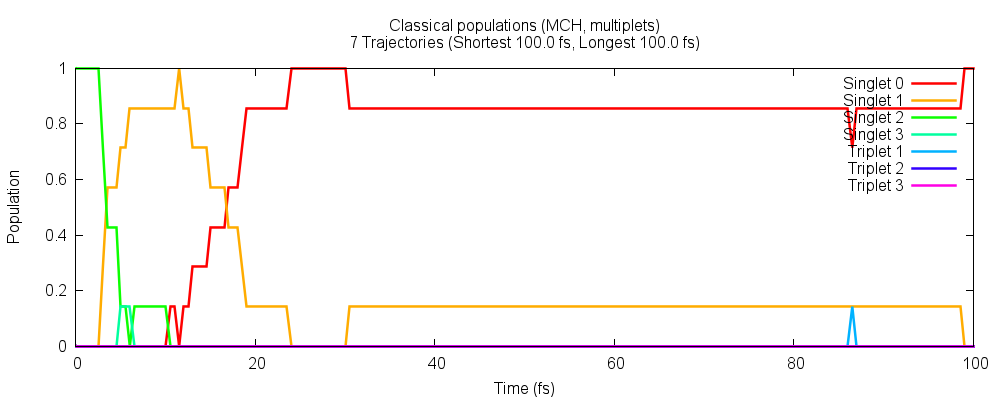
\includegraphics[width=\textwidth]{figures/pop_class.png}
  \caption{Classical populations for an ensemble of 5 trajectories.}
  \label{fig:pop_class}
\end{figure}
\begin{figure}[ptb]
  \centering
  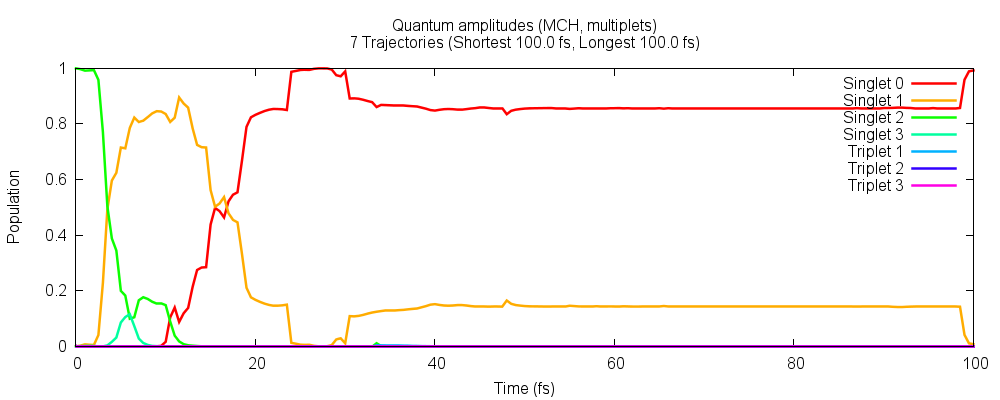
\includegraphics[width=\textwidth]{figures/pop_quant.png}
  \caption{Quantum populations for an ensemble of 5 trajectories.}
  \label{fig:pop_quant}
\end{figure}
\begin{figure}[ptb]
  \centering
  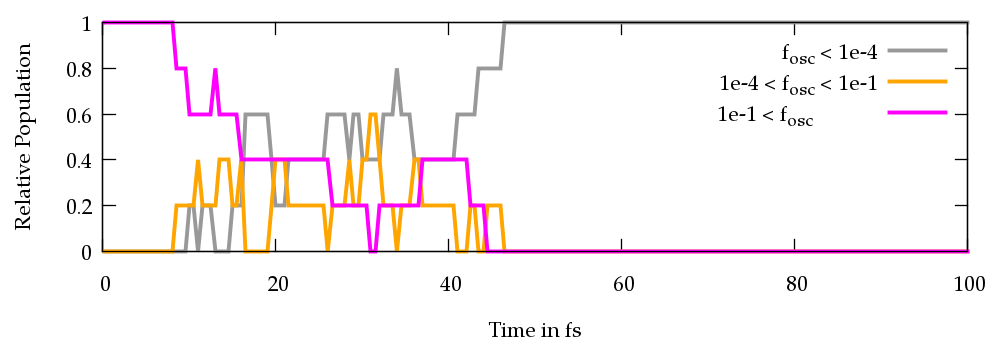
\includegraphics[width=\textwidth]{figures/pop_fosc.png}
  \caption{Populations classified based on oscillator strength for an ensemble of 5 trajectories.}
  \label{fig:pop_fosc}
\end{figure}



\paragraph{Discussion of Figure~\ref{fig:pop_class}}

In figure~\ref{fig:pop_class} it can be seen that between 0 and 30 fs, all trajectories changed from the initial $S_2$ state through the $S_1$ state to the $S_0$ ground state. The triplet states remain completely unpopulated. 

\paragraph{Discussion of Figure~\ref{fig:pop_quant}}

In figure~\ref{fig:pop_quant} the quantum populations are shown. For sufficiently large ensembles, figure~\ref{fig:pop_class} should closely follow figure~\ref{fig:pop_quant}. Consistency between the classical and quantum populations can be improved by using the decoherence correction (input option in \ttt{setup\_traj.py}).

\paragraph{Discussion of Figure~\ref{fig:pop_fosc}}

In figure~\ref{fig:pop_fosc} the ensemble population was classified according to the oscillator strength of the classically populated state. 
The chosen interval limits were 0.0001 and 0.1, giving three classes of states (below 0.0001, between 0.0001 and 0.1, and above 0.1). 
Initially, all trajectories are in the bright $\pi\pi^*$ state and are thus classified into the third class. 
During the dynamics, the dissociations/torsions/hops reduce the oscillator strength, so that the trajectories are classified into the intermediate class.
Later, the trajectories decay to the ground state, which by definition has an oscillator strength of zero (since $f_\text{osc}$ is proportional to the excitation energy). 
Note that in this example the ground state cannot be distinguished from the triplet state, which has negligible oscillator strength and thus would also be classified into the first class.
In general, however, classifying the population according to oscillator strength sometimes allows to approximately obtain populations of $\pi\pi^*$ and $n\pi^*$ states.









% ======================================================================================================

\clearpage
\subsection{Ensemble Populations Flow}
\refermanual{m-sec:transition.py}

In figure~\ref{fig:pop_class} it can be seen that, generally, population flows from the $S_2$ to the $S_1$ to the $S_0$.
In order to quantify this population flow, one can use \ttt{transition.py}.
This script counts the number of hops in all trajectories.

\begin{Verbatim}[commandchars=\\\{\}]
user@host> \textcolor{red}{$SHARC/transition.py}
\end{Verbatim}

\begin{oframed}
\footnotesize\begin{Verbatim}[commandchars=\\\{\}]
  ================================================================================
||                                                                                ||
||                   Counting hopping events from SHARC dynamics                  ||
||                                                                                ||
||                              Author: Sebastian Mai                             ||
||                                                                                ||
||                                   Version:2.0                                  ||
||                                    01.02.18                                    ||
||                                                                                ||
  ================================================================================

This script reads output.lis files files and counts all hopping events
to produce a matrix with the transition counts.
  
--------------------Paths to trajectories-------------------

Please enter the paths to all directories containing the "TRAJ_0XXXX" directories.
E.g. S_2 and S_3. 
Please enter one path at a time, and type "end" to finish the list.
Path:  [end] (autocomplete enabled) \textbf{\textcolor{red}{Singlet_2/}}
['TRAJ_00005', 'TRAJ_00004', 'TRAJ_00008', 'plot.gp', 'TRAJ_00009', 'TRAJ_00002', 
'TRAJ_00006', 'TRAJ_00010', 'TRAJ_00007', 'TRAJ_00003']
Found 9 subdirectories in total.

Path:  [end] (autocomplete enabled) \textbf{\textcolor{red}{<ENTER>}}

Total number of subdirectories: 9

------------------------Analyze Mode------------------------

This script finds the transition matrix:
1        In MCH basis                                                    from output.lis
2        In MCH basis (ignoring hops within one multiplet)               from output.lis

This script can also print the transition matrix for each timestep:
3        In MCH basis                                                    from output.lis
4        In MCH basis (ignoring hops within one multiplet)               from output.lis

Analyze mode: \textbf{\textcolor{red}{2}}

----------------------Number of states----------------------

Please enter the number of states as a list of integers
e.g. 3 0 3 for three singlets, zero doublets and three triplets.
Number of states: [4 0 3] \textbf{\textcolor{red}{<ENTER>}}

-----------------------Simulation time----------------------

Up to which simulation time should the analysis be performed?
Simulation time (in fs):  [1000.0] \textbf{\textcolor{red}{100}}


#########################Full input#########################

paths                      ['Singlet_2/']
run_extractor              False
states                     [4, 0, 3]
mode                       2
maxtime                    100.0
nstates                    7
nmstates                   13

Do you want to do the specified analysis? [True] \textbf{\textcolor{red}{<ENTER>}}

Checking the directories...
Singlet_2//TRAJ_00002         OK
Singlet_2//TRAJ_00003         OK
Singlet_2//TRAJ_00004         OK
Singlet_2//TRAJ_00005         OK
Singlet_2//TRAJ_00006         OK
Singlet_2//TRAJ_00007         OK
Singlet_2//TRAJ_00008         OK
Singlet_2//TRAJ_00009         DETECTED FILE dont_analyze
Singlet_2//TRAJ_00010         DETECTED FILE dont_analyze
Number of trajectories: 7
Number of steps: 201


***************************Results**************************
Full transition matrix:
        |      S0      S1      S2      S3      T1      T2      T3
--------+--------------------------------------------------------
  S0    |    1024       9       0       0       1       0       0
  S1    |       2     294       7       0       0       0       0
  S2    |       0       0      58       1       0       0       0
  S3    |       0       0       1       2       0       0       0
  T1    |       1       0       0       0       0       0       0
  T2    |       0       0       0       0       0       0       0
  T3    |       0       0       0       0       0       0       0

Sum transition matrix:
        |      S0      S1      S2      S3      T1      T2      T3
--------+--------------------------------------------------------
  S0    |    1024      11       0       0       2       0       0
  S1    |       0     294       7       0       0       0       0
  S2    |       0       0      58       2       0       0       0
  S3    |       0       0       0       2       0       0       0
  T1    |       0       0       0       0       0       0       0
  T2    |       0       0       0       0       0       0       0
  T3    |       0       0       0       0       0       0       0

Difference transition matrix:
        |      S0      S1      S2      S3      T1      T2      T3     Sum
--------+----------------------------------------------------------------
  S0    |       0       7       0       0       0       0       0       7
  S1    |      -7       0       7       0       0       0       0       0
  S2    |       0      -7       0       0       0       0       0      -7
  S3    |       0       0       0       0       0       0       0       0
  T1    |       0       0       0       0       0       0       0       0
  T2    |       0       0       0       0       0       0       0       0
  T3    |       0       0       0       0       0       0       0       0
  Sum   |      -7       0       7       0       0       0       0       0
\end{Verbatim}
\end{oframed}

\normalsize

The most important matrix in the output is the difference transition matrix, which shows the ``net'' hops.
In our example, it shows that there were 7 net hops from the $S_2$ to the $S_1$ and 7 net hops from the $S_1$ to the $S_0$.
No net hops occurred directly between the $S_2$ and $S_0$, or involving the triplet states.
Hence, the population flow in the ensemble is clearly $S_2\rightarrow S_1 \rightarrow S_0$.











% ======================================================================================================


\clearpage
\subsection{Fitting Ensemble Populations}
\refermanual{m-sec:make_fitscript.py}
\refermanual{m-met:globalfit}

The results in figure~\ref{fig:pop_class} show that internal conversion is an ultrafast process in \ce{CH2NH2+}.
However, in order to facilitate comparison to experiments it is useful to obtain a time constant for the relaxation processes.
\sharc\ allows fitting population data to combinations of unimolecular reactions, using \ttt{make\_fitscript.py}.
Here, we will fit the population data to the kinetic model $S_2\rightarrow S_1 \rightarrow S_0$, which was the result of the population flow analysis.
\begin{Verbatim}[commandchars=\\\{\}]
user@host> \textbf{\textcolor{red}{$SHARC/make_fitscript.py}}
\end{Verbatim}

\begin{oframed}
\footnotesize\begin{Verbatim}[commandchars=\\\{\}]
  ================================================================================
||                                                                                ||
||             Generate GNUPLOT fitting scripts for SHARC populations             ||
||                                                                                ||
||                              Author: Sebastian Mai                             ||
||                                                                                ||
||                                   Version:2.0                                  ||
||                                    01.02.18                                    ||
||                                                                                ||
  ================================================================================


This script automatizes the generation of GNUPLOT scripts for fitting of SHARC populations 
(as generated with populations.py) to general kinetic models based on first-order population transfer.


############################################################
#######################Kinetics Model#######################
############################################################


------------------------Model Species-----------------------

First, please specify the set of species used in your model kinetics.

Possible input:
+ <label> <label> ...   Adds one or several species to the set
- <label> <label> ...   Removes one or several species from the set
show                    Show the currently defined set of species
end                     Finish species input

Each label must be unique. Enter the labels without quotes.

Input: [end] \textbf{\textcolor{red}{+ S0 S1 S23}}     \textcolor{blue}{# multiple labels can be added}
  Species 'S0' added!
  Species 'S1' added!
  Species 'S23' added!                                 \textcolor{blue}{# sum of S2 and S3 for simplicity}
Input: [end] \textbf{\textcolor{red}{<ENTER>}}

Final species set:  ['S0', 'S1', 'S23']

-----------------Model Elementary Reactions-----------------

Second, please specify the set of elementary reactions in your model kinetics.

Possible input:
+ <species1> <species2> <rate_label>  Add a reaction from species1 to species2 with labelled rate constant
- <rate_label>                        Remove the reaction with the given rate constant
show                                  Show the currently defined set of reactions (as adjacency matrix)
end                                   Finish reaction input

Each rate label must be unique.

Input: [end] \textbf{\textcolor{red}{+ S23 S1 k21}}    \textcolor{blue}{# one reaction at a time}
  Reaction from 'S23' to 'S1' with rate label 'k21' added!
Input: [end] \textbf{\textcolor{red}{+ S1 S0 k10}}     \textcolor{blue}{# one reaction at a time}
  Reaction from 'S1' to 'S0' with rate label 'k10' added!
Input: [end] \textbf{\textcolor{red}{<ENTER>}}

Final reaction network:
     |  S0   S1  S23 
-----+---------------
  S0 |   .    .    . 
  S1 | k10    .    . 
 S23 |   .  k21    . 

(Initial species: rows; Final species: columns)

------------------Model Initial Conditions------------------

Third, please specify species with non-zero initial populations.

Possible input:
+ <species>       Declare species to have non-zero initial population
- <species>       Remove species from the set of non-zero initial populations
show              Show the currently defined non-zero initial populations
end               Finish initial condition input

Input: [end] \textbf{\textcolor{red}{+ S23}}         \textcolor{blue}{# initial population is in S2}
  Species 'S23' added!
Input: [end] \textbf{\textcolor{red}{<ENTER>}}

Final initial species set:  ['S23']

############################################################
########################Fitting Data########################
############################################################


--------------------Population data file--------------------

Please specify the path to the population data file (as generated by populations.py).

Populations file: [pop.out] (autocomplete enabled) \textbf{\textcolor{red}{<ENTER>}}
  Detected maximal time of   100.0 fs and 8 columns (time plus 7 data columns).

------------Population-to-Species Mapping for Fit-----------

Please specify which model species should be fitted to which data file columns.
For example, you can fit the label 'S0' to column 2:
  S0 = 2
You can also fit the sum of two species to a column:
  T1 T2 = 5
You can also fit a species to the sum of several columns:
  T_all = 5 6 7
You can even fit a sum of species to a sum of columns:
  T1 T2 = 5 6 7

Possible input:
<species1> <species2> ... = <columns1> <column2> ...            Set one mapping
show                                                            Show mapping
end                                                             Finish mapping input
reset                                                           Redo the mapping input

Each species label must be used at most once.
Each column number (except for '1', which denotes the time) must be used at most once.

Set of species:        ['S0', 'S1', 'S23']
Set of column numbers: [2, 3, 4, 5, 6, 7, 8]
Input: [end] \textbf{\textcolor{red}{S0 = 2}}       \textcolor{blue}{# fit S0 to column 2 data}
Input: [end] \textbf{\textcolor{red}{S1 = 3}}       \textcolor{blue}{# fit S1 to column 3 data}
Input: [end] \textbf{\textcolor{red}{S23 = 4 5}}    \textcolor{blue}{# fit S23 to sum of column 4 and 5}
Input: [end] \textbf{\textcolor{red}{<ENTER>}}
Final mappings:
     S0  =  2 
     S1  =  3 
     S23  =  4  5 


#########################Full input#########################

initset                    set(['S23'])
ngroups                    3
species_groups             [['S0'], ['S1'], ['S23']]
rank                       0
rateset                    set(['k10', 'k21'])
columns_groups             [[2], [3], [4, 5]]
ncol                       8
rate_matrix                [['', '', ''], ['k10', '', ''], ['', 'k21', '']]
specmap                    {0: 'S0', 1: 'S1', 2: 'S23', 'S1': 1, 'S0': 0, 'S23': 2}
popfile                    /user/mai/Documents/NewSHARC/SHARC_2.0/TUTORIAL/2_full/Tutorial/traj/pop.out
nspec                      3
data                       [ ... ]
maxtime                    100.0

Do you want to continue? [True] \textbf{\textcolor{red}{<ENTER>}}

Calling MAXIMA computer algebra system with following command:
  maxima -b /user/mai/Documents/NewSHARC/SHARC_2.0/TUTORIAL/2_full/Tutorial/traj/MAXIMA.input
Run this command? [True] \textbf{\textcolor{red}{<ENTER>}}


Running MAXIMA...               \textcolor{blue}{# this will only work if you have Maxima installed}
Done!
Writing GNUPLOT script to model_fit.gp ...
Writing GNUPLOT populations data to model_fit.dat ...

**************************************************************
*                Final Instructions and Hints                *    \textcolor{blue}{# read these hints}
**************************************************************

* How to run the fit *
  The fitting script is a script for GNUPLOT. Execute it with:
    user@host> gnuplot model_fit.gp
  Note that the file "model_fit.dat" must be present for the GNUPLOT script to work.
  By pressing ENTER, you can proceed through these stages:
    1) Initial plot of the population data and the fitting functions using the initial fitting parameters
    2) Plot of the data and functions (transformed for global fit) before fitting
    3) Perform the global fit and plot of the data and functions
    4) Final plot of the population data and the fitting functions, also presenting the final fit parameters
    5) Write the final plot to "model_fit.png" and write the data to "model_fit.txt"

* Adjust initial parameters *
  Please adjust the starting guess values of the following fitting parameters:
    k10
    k21
    S23__0
  in file "model_fit.gp" before running the fitting procedure.

* Fitting of initial populations *
  The fitting script was setup to only optimize the rate constants in the global fit.
  If you intend to also optimize the initial populations, please modify the fit command like this:
    fit F(x) [...] via k10,k21,S23__0

**** Unused species or data columns ****
  The population data file contains columns which are not used in the global fit:
    6
    7
    8
  Please ensure that this is in accord with your intentions.
**************************************************************
\end{Verbatim}
\end{oframed}

\normalsize

The script writes two new files, \ttt{model\_fit.gp} and \ttt{model\_fit.dat}.
The former is a \textsc{Gnuplot} script which can be executed to carry out the population fit.
You should inspect this file; in particular, note the initial guesses for the fit in a section which looks like this:
\begin{oframed}
\footnotesize\begin{Verbatim}[commandchars=\\\{\}]
# *** Reaction rates initial guesses: ***
# These are given in units of inverse fs (e.g., time constant of 100 fs is written as 1./100.).
# TODO: Please change to some suitable values!
k10 = 1./100.
k21 = 1./101.

# *** Species population initial guesses: ***
# TODO: Please change to some suitable values!
S23__0 = 1./1.
\end{Verbatim}
\end{oframed}

\normalsize
In general, it might be necessary to change these initial parameters in order to make the fit converge, but here in the tutorial, the default values should be fine.

Run \textsc{Gnuplot} to carry out the fit (use \textcolor{red}{\ttt{<ENTER>}} to advance through the script):
\begin{Verbatim}[commandchars=\\\{\}]
user@host> \textbf{\textcolor{red}{$SHARC/make_fitscript.py}}
\end{Verbatim}
At the end, the script produces a figure, \ttt{model\_fit.png}, which presents the results of the fit.
The second output file, \ttt{model\_fit.txt}, can be used to prepare visually more appealing plots of the fit for production purposes.
The result of the fit is shown in Figure~\ref{fig:model_fit}.

\begin{figure}[ptb]
  \centering
  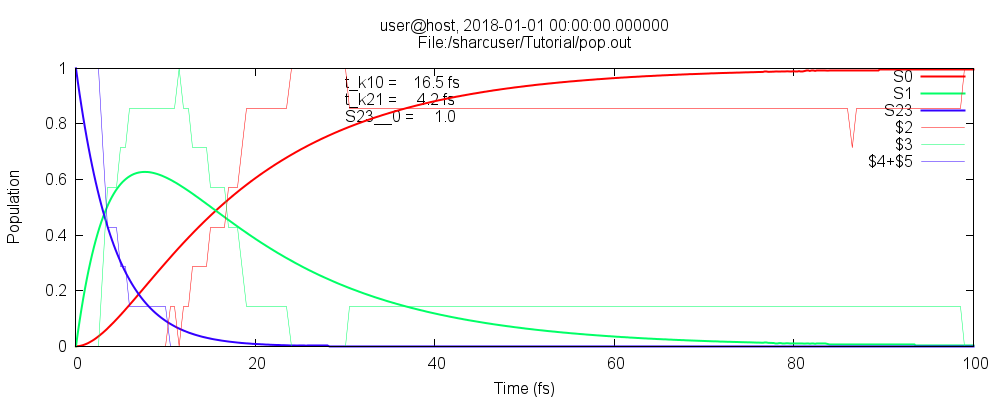
\includegraphics[width=\textwidth]{figures/model_fit.png}
  \caption{Kinetic model fit of the classical populations.}
  \label{fig:model_fit}
\end{figure}

\paragraph{Discussion of Figure~\ref{fig:model_fit}}

From the figure, it can be seen that the $S_2\rightarrow S_1$ time constant is 4.2~fs, and the time constant for $S_1\rightarrow S_0$ is 16.5~fs.
Note that the fit is not very good, because the number of trajectories is low and the relaxation processes in \ce{CH2NH2+} are so fast that first-order reactions are not optimal to describe them.
For slower processes in larger molecules, these kinetic model fits might work better.





% ======================================================================================================

\clearpage
\subsection{Fitting Ensemble Populations: Error Estimation}
\refermanual{m-sec:bootstrap.py}
\refermanual{m-met:bootstrapping}

In order to obtain error estimates of the time constants fitted using \ttt{make\_fitscript.py}, one can use the bootstrapping method.
In this method, based on the original ensemble (of 7 trajectories), ``resample'' ensembles are generated by randomly drawing \emph{with replacement} trajectories from the original ensemble (here, drawing 7 random trajectories).
Each resample is then fitted in exactly the same way as the original ensemble, and after many resamples a distribution of possible fitting parameters is obtained.
From this distribution, one can then find error measures for the fitting parameters.

Start \ttt{bootstrap.py} by:
\begin{Verbatim}[commandchars=\\\{\}]
user@host> \textbf{\textcolor{red}{$SHARC/bootstrap.py}}
\end{Verbatim}

\begin{oframed}
\footnotesize\begin{Verbatim}[commandchars=\\\{\}]
  ================================================================================
||                                                                                ||
||                  Bootstrap time constants from SHARC dynamics                  ||
||                                                                                ||
||                              Author: Sebastian Mai                             ||
||                                                                                ||
||                                   Version:2.0                                  ||
||                                    01.02.18                                    ||
||                                                                                ||
  ================================================================================


This script reads ensemble populations (from populations.py) and a kinetic model (from make_fitscript.py)
and computes statistics on the kinetic model fitting.
  
-------------------Paths to bootstrap data------------------

Please enter the path to the directory containing the raw bootstrap data.
This data can be generated with populations.py

Path:  [bootstrap_data/] (autocomplete enabled) \textbf{\textcolor{red}{<ENTER>}}
['pop_1.dat', 'pop_5.dat', 'pop_4.dat', 'pop_6.dat', 'pop_7.dat', 'pop_2.dat', 'pop_3.dat']
Found 7 bootstrap data files.

-----------------Number of bootstrap cycles-----------------

Please enter the number of bootstrapping cycles to be performed.
Number of bootstrap cycles:  [10] \textbf{\textcolor{red}{500}}

Please enter a random number generator seed (type "!" to initialize the RNG from the system time).
RNG Seed:  [!] \textbf{\textcolor{red}{1234}}

-----------------------Fitting script-----------------------

Please provide the path to the desired fitting script.
This script can be generated with make_fitscript.py, and should subsequently me adjusted (suitable 
guesses for fitted constants).
Path:  [model_fit.gp] (autocomplete enabled) \textbf{\textcolor{red}{<ENTER>}}

Please provide the command to execute gnuplot.
Command:  [gnuplot] (autocomplete enabled) \textbf{\textcolor{red}{<ENTER>}}

--------------------Parallel computation--------------------

bootstrap.py can run the fitting (which is done through Gnuplot) on multiple CPU).
(however, the overhead is currently large, so speedup is limited)
Number of CPUs to use:  [1] \textbf{\textcolor{red}{<ENTER>}}

#########################Full input#########################

ntraj                   7
gnuplot                 gnuplot
fitfile                 /user/mai/Documents/NewSHARC/SHARC_2.0/TUTORIAL/2_full/Tutorial/traj/model_fit.gp
nboot                   500
ncpu                    1
bootstrap_dir           /user/mai/Documents/NewSHARC/SHARC_2.0/TUTORIAL/2_full/Tutorial/traj/bootstrap_data
ncol                    7
npercycle               22
steps                   200
dt                      0.5

Do you want to do the specified analysis? [True] 

>>>>>>>>>>>>> Reading the ensemble data ...
0 /user/mai/Documents/NewSHARC/SHARC_2.0/TUTORIAL/2_full/Tutorial/traj/bootstrap_data/pop_1.dat
1 /user/mai/Documents/NewSHARC/SHARC_2.0/TUTORIAL/2_full/Tutorial/traj/bootstrap_data/pop_2.dat
2 /user/mai/Documents/NewSHARC/SHARC_2.0/TUTORIAL/2_full/Tutorial/traj/bootstrap_data/pop_3.dat
3 /user/mai/Documents/NewSHARC/SHARC_2.0/TUTORIAL/2_full/Tutorial/traj/bootstrap_data/pop_4.dat
4 /user/mai/Documents/NewSHARC/SHARC_2.0/TUTORIAL/2_full/Tutorial/traj/bootstrap_data/pop_5.dat
5 /user/mai/Documents/NewSHARC/SHARC_2.0/TUTORIAL/2_full/Tutorial/traj/bootstrap_data/pop_6.dat
6 /user/mai/Documents/NewSHARC/SHARC_2.0/TUTORIAL/2_full/Tutorial/traj/bootstrap_data/pop_7.dat

>>>>>>>>>>>>> Starting the bootstrapping cycles ...
             (use Ctrl-C to skip the remaining cycles and go to the final analysis)

Step |       Run Time |    Key: g.Mean     g.Stdv | ...
=======================================================
  22 | 0:00:03.216253 | S23__0:   1.00 +/-   0.00 | k10:   15.68 +/-   7.65 | k21:   4.33 +/-   0.93 
  44 | 0:00:03.169761 | S23__0:   1.00 +/-   0.00 | k10:   16.77 +/-   8.77 | k21:   4.30 +/-   0.96 
  66 | 0:00:03.117776 | S23__0:   1.00 +/-   0.00 | k10:   18.30 +/-  11.47 | k21:   4.26 +/-   0.94 
  88 | 0:00:03.256217 | S23__0:   1.00 +/-   0.00 | k10:   17.80 +/-  10.37 | k21:   4.22 +/-   0.90 
 110 | 0:00:03.252534 | S23__0:   1.00 +/-   0.00 | k10:   18.20 +/-  11.09 | k21:   4.20 +/-   0.96 
 132 | 0:00:03.259927 | S23__0:   1.00 +/-   0.00 | k10:   18.45 +/-  11.28 | k21:   4.18 +/-   0.94 
 154 | 0:00:03.295209 | S23__0:   1.00 +/-   0.00 | k10:   18.07 +/-  11.05 | k21:   4.20 +/-   0.97 
 176 | 0:00:03.131462 | S23__0:   1.00 +/-   0.00 | k10:   18.18 +/-  11.20 | k21:   4.16 +/-   0.96 
 198 | 0:00:03.241862 | S23__0:   1.00 +/-   0.00 | k10:   17.85 +/-  10.80 | k21:   4.19 +/-   0.98 
 220 | 0:00:03.218833 | S23__0:   1.00 +/-   0.00 | k10:   17.69 +/-  10.44 | k21:   4.20 +/-   0.97 
 242 | 0:00:03.381416 | S23__0:   1.00 +/-   0.00 | k10:   18.10 +/-  11.26 | k21:   4.17 +/-   0.99 
 264 | 0:00:03.197810 | S23__0:   1.00 +/-   0.00 | k10:   18.21 +/-  11.44 | k21:   4.17 +/-   0.99 
 286 | 0:00:03.264219 | S23__0:   1.00 +/-   0.00 | k10:   18.32 +/-  11.53 | k21:   4.16 +/-   0.99 
 308 | 0:00:03.188074 | S23__0:   1.00 +/-   0.00 | k10:   18.22 +/-  11.14 | k21:   4.19 +/-   0.98 
 330 | 0:00:03.201072 | S23__0:   1.00 +/-   0.00 | k10:   18.23 +/-  11.07 | k21:   4.18 +/-   0.98 
 352 | 0:00:03.258426 | S23__0:   1.00 +/-   0.00 | k10:   18.33 +/-  11.30 | k21:   4.18 +/-   0.98 
 374 | 0:00:03.262513 | S23__0:   1.00 +/-   0.00 | k10:   18.32 +/-  11.22 | k21:   4.18 +/-   0.98 
 396 | 0:00:03.201724 | S23__0:   1.00 +/-   0.00 | k10:   18.41 +/-  11.67 | k21:   4.17 +/-   0.99 
 418 | 0:00:03.307559 | S23__0:   1.00 +/-   0.00 | k10:   18.50 +/-  11.75 | k21:   4.15 +/-   0.99 
 440 | 0:00:03.274169 | S23__0:   1.00 +/-   0.00 | k10:   18.47 +/-  11.72 | k21:   4.15 +/-   0.98 
 462 | 0:00:03.382566 | S23__0:   1.00 +/-   0.00 | k10:   18.55 +/-  11.84 | k21:   4.14 +/-   0.98 
 484 | 0:00:03.272651 | S23__0:   1.00 +/-   0.00 | k10:   18.54 +/-  11.88 | k21:   4.14 +/-   0.98 
 500 | 0:00:02.428860 | S23__0:   1.00 +/-   0.00 | k10:   18.48 +/-  11.78 | k21:   4.14 +/-   0.97 
Run time = 0:01:13.782832

>>>>>>>>>>>>> Finished the bootstrapping cycles ...









---------------------------------- Analysis for time constant "S23__0" ------------------------------------

  Arithmetic analysis:              1.000000 +/-     0.000000
                                           ( +/-       0.00 %)

  Geometric analysis:               1.000000  +      0.000000  -     -0.000000
                                           (  +        0.00 %  -       -0.00 %)

  Minimum and maximum:              1.000000      and           1.000000

  Histogram:
  ==========
     #                                                            | 500
     #                                                            | 458
     #                                                            | 416
     #                                                            | 375
     #                                                            | 333
     #                                                            | 291
     #                                                            | 250
     #                                                            | 208
     #                                                            | 166
     #                                                            | 125
     #                                                            | 83
     #                                                            | 41
        |     |     |     |     |     |     |     |     |     |  
    1.000 1.000 1.000 1.000 1.000 1.000 1.000 1.000 1.000 1.000

----------------------------------- Analysis for time constant "k10" --------------------------------------

  Arithmetic analysis:             21.283774 +/-    13.641992
                                           ( +/-      64.10 %)

  Geometric analysis:              18.483510  +     11.777237  -      7.193632
                                           (  +       63.72 %  -       38.92 %)

  Minimum and maximum:              8.411113      and          89.459494

  Histogram:
  ==========
                                   #                              | 157
                             #     #                              | 143
                             #     #                              | 130
                             #     #                              | 117
                             #     #                              | 104
                             #     #                              | 91
                             #     #           #                  | 78
                             #     #           #                  | 65
                             #     #           #                  | 52
                             #     #           #                  | 39
                             #     #     #     #           #      | 26
                       #     #     #     #     #           #      | 13
        |     |     |     |     |     |     |     |     |     |  
    4.212 5.662 7.610 10.23 13.75 18.48 24.85 33.40 44.89 60.34

    
    
    
    
    
----------------------------------- Analysis for time constant "k21" --------------------------------------

  Arithmetic analysis:              4.231712 +/-     0.926623
                                           ( +/-      21.90 %)

  Geometric analysis:               4.136707  +      0.974861  -      0.788939
                                           (  +       23.57 %  -       19.07 %)

  Minimum and maximum:              2.409199      and           7.829985

  Histogram:
  ==========
                                   #                              | 124
                                   #                              | 113
                                   #                              | 103
                                   #     #                        | 93
                             #     #     #                        | 82
                             #     #     #     #                  | 72
                             #     #     #     #                  | 62
                             #     #     #     #                  | 51
                       #     #     #     #     #                  | 41
                       #     #     #     #     #     #            | 31
                       #     #     #     #     #     #            | 20
                       #     #     #     #     #     #     #      | 10
        |     |     |     |     |     |     |     |     |     |  
    2.193 2.489 2.826 3.209 3.643 4.137 4.697 5.333 6.054 6.874

Output (analysis and full fitted data) written to "bootstrap.out".

\end{Verbatim}
\end{oframed}

\normalsize

While the script is running, it prints the intermediate results of the bootstrapping procedure.
Note that if the bootstrapping iterations take too long and the results seem to be converged already, pressing \ttt{Ctrl+C} allows skipping the remaining iterations and directly leads to the final analysis.

The result of the bootstrapping procedure is presented in a summary for each fitting parameter.
Note that by default also the initial populations are treated as fitting parameters, even if they are fixed in the shown example.

The results show that the $S_2\rightarrow S_1$ relaxation process in the trajectories had a time constant of 4.2$\pm$0.9~fs (using the arithmetic analysis).
Most fits yielded a time constant between 3 and 6~fs.

For the $S_1\rightarrow S_0$ process, the result is 21.3$\pm$13.6~fs.
According to the histogram, most of the fits yielded a value between 13 and 20~fs, although there were many fits with values around 30~fs and even some above 50~fs.
This broad distribution leads to the large error found.
Clearly, it is due to the small number of trajectories---it is very likely that in some resamples one particular trajectory is missing, which leads to a large change of the fitted parameters.
Also note that the distribution of this parameter is very skewed (with a long right tail); in this situation it might be preferable to use the results of the geometric analysis (which gives $18.4\substack{+11.8\\-7.2}$~fs).

Generally, the errors get smaller as more trajectories are employed, and hence, the fitting errors are a good tool to judge whether enough trajectories were computed.
However, the obtained errors tell nothing about the inherent method error---using surface hopping in combination with a given quantum chemistry method.
It is not possible to quantify this method error with \ttt{bootstrap.py}; only through comparison with reference data or experiment can the method error be judged.










% ======================================================================================================

\clearpage
\subsection{Hopping Geometries}
\refermanual{m-sec:crossing.py}

Another aspect one might be interested in are certain critical geometries from the trajectories.
\ttt{crossing.py} is a script that collects those geometries from all trajectories where a surface hop between two specified states occurred.
Its usage is comparable to \ttt{populations.py}.
\begin{Verbatim}[commandchars=\\\{\}]
user@host> \textbf{\textcolor{red}{$SHARC/crossing.py}}
\end{Verbatim}

\begin{oframed}
\footnotesize\begin{Verbatim}[commandchars=\\\{\}]
  ================================================================================
||                                                                                ||
||                 Reading hopping geometries from SHARC dynamics                 ||
||                                                                                ||
||                              Author: Sebastian Mai                             ||
||                                                                                ||
||                                   Version:2.0                                  ||
||                                    01.02.18                                    ||
||                                                                                ||
  ================================================================================


This script reads output.lis files and output.xyz files to produce a list of
all geometries where certain surface hops (or other events) occured.

--------------------Paths to trajectories-------------------

Please enter the paths to all directories containing the "TRAJ_0XXXX" directories.
E.g. S_2 and S_3.
Please enter one path at a time, and type "end" to finish the list.
Path:  [end] (autocomplete enabled) \textbf{\textcolor{red}{Singlet_2/}}
['TRAJ_00005', 'TRAJ_00004', 'TRAJ_00008', 'plot.gp', 'TRAJ_00009', 'TRAJ_00002', 
'TRAJ_00006', 'TRAJ_00010', 'TRAJ_00007', 'TRAJ_00003']
Found 9 subdirectories in total.

Path:  [end] (autocomplete enabled) \textbf{\textcolor{red}{<ENTER>}}

Total number of subdirectories: 9

------------------------Analyze Mode------------------------

This script can find geometries where:
1        A change of MCH state occured (ignoring hops within one multiplet)               from output.lis

Analyze mode: \textbf{\textcolor{red}{1}}

----------------------Number of states----------------------

Please enter the number of states as a list of integers
e.g. 3 0 3 for three singlets, zero doublets and three triplets.
Number of states: [4 0 3] \textbf{\textcolor{red}{<ENTER>}}


---------------States involved in surface hop---------------

In this analysis mode, all geometries are fetched where a trajectory switches from a given MCH state
to another given MCH state.

Please enter the old MCH state involved as "mult state", e.g., "1 1" for S0, "1 2" for S1, or "3 1" for T1:
State 1: \textbf{\textcolor{red}{1  2}}      \textcolor{blue}{# Only hops from S1}

Please enter the new MCH state involved (mult state):
State 2: \textbf{\textcolor{red}{1  1}}      \textcolor{blue}{# to S0}

Direction:
1       Forwards      \textcolor{blue}{# Only S1 -> S0}
2       Backwards     \textcolor{blue}{# Only S0 -> S1}
3       Two-way       \textcolor{blue}{# Both S1 -> S0 and S0 -> S1}

Direction mode: [3] \textbf{\textcolor{red}{1}}

#########################Full input#########################

paths                      ['Singlet_2/']
tostates                   [[1, 1], [1, 2]]
run_extractor              False
states                     [4, 0, 3]
mode                       1
dirmode                    1
nstates                    7
fromstates                 [[1, 1], [1, 2]]
nmstates                   13

Do you want to do the specified analysis? [True] \textbf{\textcolor{red}{<ENTER>}}

Checking the directories...
Singlet_2//TRAJ_00002         OK
Singlet_2//TRAJ_00003         OK
Singlet_2//TRAJ_00004         OK
Singlet_2//TRAJ_00005         OK
Singlet_2//TRAJ_00006         OK
Singlet_2//TRAJ_00007         OK
Singlet_2//TRAJ_00008         OK
Singlet_2//TRAJ_00009         DETECTED FILE dont_analyze
Singlet_2//TRAJ_00010         DETECTED FILE dont_analyze
Number of trajectories: 7

Writing to crossing.xyz ...
\end{Verbatim}
\end{oframed}

\normalsize
The script writes a files called \ttt{crossing.xyz}, which contains all geometries (9 geometries in this example) where a hop from the $S_1$ to the $S_0$ occurred.
This file can in turn be analyzed with \ttt{geo.py} in order to calculate internal coordinates (e.g., to find whether a bond or angle controls access to the $S_1/S_0$ crossing seam, or how many different pathways allow this transition). 

% ======================================================================================================

\clearpage
\subsection{Optimizing from Hopping Geometries}
\refermanual{m-sec:Orca_External}
\refermanual{m-met:orcaopt}

The output of \ttt{crossing.py} can also be used to optimize minimum-energy crossing points and conical intersections (e.g., to find how many independent crossing seam regions, i.e., reaction pathways, are involved).
In \sharc, this optimization can be automatically setup if \textsc{Orca} is installed (\textsc{Orca} is needed to perform the actual optimization of the nuclei, whereas \sharc\ provides the necessary energies and gradients).

The setup of the optimizations can be started with 
\begin{Verbatim}[commandchars=\\\{\}]
user@host> \textbf{\textcolor{red}{$SHARC/setup_orca_opt.py}}
\end{Verbatim}

\begin{oframed}
\footnotesize\begin{Verbatim}[commandchars=\\\{\}]
  ================================================================================
||                                                                                ||
||                     Setup optimizations with ORCA and SHARC                    ||
||                                                                                ||
||                      Author: Moritz Heindl, Sebastian Mai                      ||
||                                                                                ||
||                                   Version:2.0                                  ||
||                                    01.02.18                                    ||
||                                                                                ||
  ================================================================================

This script automatizes the setup of the input files ORCA+SHARC optimizations. 
  
------------------------Path to ORCA------------------------

Please specify path to ORCA directory (SHELL variables and ~ can be used, 
will be expanded when interface is started).

Path to ORCA: [$ORCADIR/] (autocomplete enabled) \textbf{\textcolor{red}{<ENTER>}}

-----------Choose the quantum chemistry interface-----------

Please specify the quantum chemistry interface (enter any of the following numbers):
1       MOLPRO (only CASSCF)
2       COLUMBUS (CASSCF, RASSCF and MRCISD), using SEWARD integrals
3       Analytical PESs
4       MOLCAS (CASSCF, CASPT2, MS-CASPT2)
5       ADF (DFT, TD-DFT)
6       TURBOMOLE (ricc2 with CC2 and ADC(2))
7       LVC Hamiltonian
8       GAUSSIAN (DFT, TD-DFT)

Interface number: \textbf{\textcolor{red}{4}}

--------------------------Geometry--------------------------

Please specify the geometry file (xyz format, Angstroms):
Geometry filename: [geom.xyz] (autocomplete enabled) \textbf{\textcolor{red}{crossing.xyz}}
Number of geometries: 9

----------------------Number of states----------------------


Please enter the number of states as a list of integers
e.g. 3 0 3 for three singlets, zero doublets and three triplets.
Number of states: \textbf{\textcolor{red}{4  0  3}}

Number of states: [4, 0, 3]
Total number of states: 13

\{1: [1, 1, 0.0],
 2: [1, 2, 0.0],
 3: [1, 3, 0.0],
 4: [1, 4, 0.0],
 5: [3, 1, -1.0],
 6: [3, 2, -1.0],
 7: [3, 3, -1.0],
 8: [3, 1, 0.0],
 9: [3, 2, 0.0],
 10: [3, 3, 0.0],
 11: [3, 1, 1.0],
 12: [3, 2, 1.0],
 13: [3, 3, 1.0]\}

---------------------States to optimize---------------------

Do you want to optimize a minimum? (no=optimize crossing): [True] \textbf{\textcolor{red}{no}}

Please specify the first state involved in the optimization
e.g. 3 2 for the second triplet state.
State: [1 1] \textbf{\textcolor{red}{<ENTER>}}

Please specify the second state involved in the optimization
e.g. 3 2 for the second triplet state.
Root: [1 2] \textbf{\textcolor{red}{<ENTER>}}
Multiplicities of both states identical, optimizing a conical intersection.

-------------------Optimization parameter-------------------

You are optimizing a conical intersection, but the chosen interface cannot deliver 
nonadiabatic coupling vectors. The optimization will therefore employ the penalty 
function method of Levine, Coe, Martinez (DOI: 10.1021/jp0761618).
In this optimization scheme, there are two parameters, sigma and alpha, which affect 
how close to the true conical intersection the optimization will end up.

Please enter the values for the sigma and alpha parameters.

A larger sigma makes convergence harder but optimization will go closer to the true CI.
Sigma:  [3.5] \textbf{\textcolor{red}{<ENTER>}}
A smaller alpha makes convergence harder but optimization will go closer to the true CI.
Alpha:  [0.02] \textbf{\textcolor{red}{<ENTER>}}

Please enter the values for the maximum allowed displacement per timestep 
(choose smaller value if starting from a good guess and for large sigma or small alpha).
Maximum allowed step:  [0.3] \textbf{\textcolor{red}{<ENTER>}}

  ================================================================================
||                             MOLCAS Interface setup                             ||
  ================================================================================

-----------------------Path to MOLCAS-----------------------

Please specify path to MOLCAS directory (SHELL variables and ~ can be used, 
will be expanded when interface is started).

Path to MOLCAS: [$MOLCAS/] (autocomplete enabled) \textbf{\textcolor{red}{<ENTER>}}

----------------------Scratch directory---------------------

Please specify an appropriate scratch directory. This will be used to temporally 
store the integrals. The scratch directory will be deleted after the calculation. 
Remember that this script cannot check whether the path is valid, since you may 
run the calculations on a different machine. The path will not be expanded by this script.
Path to scratch directory: (autocomplete enabled) \textbf{\textcolor{red}{$TMPDIR}}

-----------------MOLCAS input template file-----------------

Please specify the path to the MOLcas.template file. This file must contain the following settings:

basis <Basis set>
ras2 <Number of active orbitals>
nactel <Number of active electrons>
inactive <Number of doubly occupied orbitals>
roots <Number of roots for state-averaging>

The MOLCAS interface will generate the appropriate MOLCAS input automatically.

Template filename: (autocomplete enabled) \textbf{\textcolor{red}{../MOLCAS.template}}

---------------Initial wavefunction: MO Guess---------------

Please specify the path to a MOLCAS JobIph file containing suitable starting MOs for 
the CASSCF calculation. Please note that this script cannot check whether the 
wavefunction file and the Input template are consistent!

Do you have initial wavefunction files for Singlet, Triplet? [True] \textbf{\textcolor{red}{<ENTER>}}
JobIph files (1) or RasOrb files (2)? \textbf{\textcolor{red}{2}}
Initial wavefunction file for Singlets: [MOLCAS.1.RasOrb.init] (autocomplete enabled) \textbf{\textcolor{red}{../MOLCAS.RasOrb}}
Initial wavefunction file for Triplets: [MOLCAS.3.RasOrb.init] (autocomplete enabled) \textbf{\textcolor{red}{../MOLCAS.RasOrb}}

-------------------MOLCAS Ressource usage-------------------

Please specify the amount of memory available to MOLCAS (in MB). For calculations including
moderately-sized CASSCF calculations and less than 150 basis functions, around 2000 MB should be sufficient.

MOLCAS memory: \textbf{\textcolor{red}{1000}}
Please specify the number of CPUs to be used by EACH calculation.

Number of CPUs: \textbf{\textcolor{red}{1}}

  ================================================================================
||                                 Run mode setup                                 ||
  ================================================================================

-------------------------Run script-------------------------

Where do you want to perform the calculations? Note that this script cannot check whether the path is valid.
Run directory? (autocomplete enabled) \textbf{\textcolor{red}{orca_opt/}}


#########################Full input#########################

molcas                     $MOLCAS/
states                     [4, 0, 3]
molcas.jobiph_or_rasorb    2
geom_location              crossing.xyz
nstates                    13
molcas.ncpu                1
calc_ci                    True
molcas.guess               \{1: '../MOLCAS.RasOrb', 3: '../MOLCAS.RasOrb'\}
scratchdir                 $TMPDIR
opttype                    cross
needed                     []
ngeom                      11
cwd                        /user/mai/Documents/NewSHARC/SHARC_2.0/TUTORIAL/2_full/Tutorial/traj
molcas.template            ../MOLCAS.template
maxstep                    0.3
cas.root1                  1
cas.root2                  2
maxmult                    3
here                       False
statemap                   \{1: [1, 1, 0.0], 
                            2: [1, 2, 0.0], 
                            3: [1, 3, 0.0], 
                            4: [1, 4, 0.0], 
                            5: [3, 1, -1.0], 
                            6: [3, 2, -1.0], 
                            7: [3, 3, -1.0], 
                            8: [3, 1, 0.0], 
                            9: [3, 2, 0.0], 
                            10: [3, 3, 0.0], 
                            11: [3, 1, 1.0], 
                            12: [3, 2, 1.0], 
                            13: [3, 3, 1.0]\}
interface                  4
alpha                      0.02
copydir                    orca_opt
molcas.mem                 1000
natom                      6
sigma                      3.5
orca                       $ORCADIR/

Do you want to setup the specified calculations? [True] \textbf{\textcolor{red}{<ENTER>}}

  ================================================================================
||                             Setting up directory...                            ||
  ================================================================================
\end{Verbatim}
\end{oframed}

\normalsize
The script will create 9 subdirectories in the given setup directory, \ttt{orca\_opt/}.
Each of these 9 directories will contain the input files for an optimization using \textsc{Orca}'s external optimizer feature, where the energies and gradients will be provided by \ttt{\$SHARC/orca\_External} (this is done automatically), which itself calls the \textsc{Molcas} interface to do the computations.

In order to run one of these optimizations, execute:
\begin{Verbatim}[commandchars=\\\{\}]
user@host> \textbf{\textcolor{red}{cd orca_opt/geom_9/}}
user@host> \textbf{\textcolor{red}{sh run_EXTORCA.sh&}}
\end{Verbatim}
The progress of the optimization can be followed in \ttt{orca.log}. In this file, note the lines following \ttt{EXTERNAL SHARC JOB}, which are written by \sharc\ and show the computed energies and gradients.
Close to a box labeled \ttt{Geometry convergence}, \textsc{Orca} reports the convergence status of the optimization.
After 25~cycles, the optimization should converge; the energies of $S_0$ and $S_1$ at convergence should be $-94.263728$ and $-94.263586$~Hartree.
This is a very good result, as the energy gap is only 0.004~eV; if the gap was much larger, then the optimization should be repeated (starting from the last step) with adjusted optimization parameters (\ttt{Sigma} and \ttt{Alpha}, see also the manual).




% ======================================================================================================

\clearpage
\subsection{Essential Dynamics Analysis}
\refermanual{m-sec:trajana_essdyn.py}
\refermanual{m-met:essdyn}

Another possibility to investigate nuclear motion in the trajectories is given by the essential dynamics analysis.
This analysis simply takes all trajectories and identifies collective motion, which can be useful to find reaction paths or to construct reduced-dimensionality models.

The interactive script can be started with 
\begin{Verbatim}[commandchars=\\\{\}]
user@host> \textbf{\textcolor{red}{$SHARC/trajana_essdyn.py}}
\end{Verbatim}

\begin{oframed}
\footnotesize\begin{Verbatim}[commandchars=\\\{\}]
  ================================================================================
||                                                                                ||
||                 Essential dynamics analysis for SHARC dynamics                 ||
||                                                                                ||
||                      Author: Felix Plasser, Andrew Atkins                      ||
||                                                                                ||
||                                   Version:2.0                                  ||
||                                    01.02.18                                    ||
||                                                                                ||
  ================================================================================


This script reads output.xyz files and calculates the essential dynamics 
(i.e., Shows you which are the most important motions).
  
--------------------Paths to trajectories-------------------

Please enter the paths to all directories containing the "TRAJ_0XXXX" directories.
E.g. Sing_2/ and Sing_3/. 
Please enter one path at a time, and type "end" to finish the list.
Path:  [end] (autocomplete enabled) \textbf{\textcolor{red}{Singlet_2/}}
['TRAJ_00005', 'TRAJ_00004', 'TRAJ_00008', 'plot.gp', 'TRAJ_00009', 'TRAJ_00002', 
'TRAJ_00006', 'TRAJ_00010', 'TRAJ_00007', 'TRAJ_00003']
Found 9 subdirectories in total.

Path:  [end] (autocomplete enabled) \textbf{\textcolor{red}{<ENTER>}}

Total number of subdirectories: 9

-----------------Path to reference structure----------------

Please enter the path to the equilibrium structure of your system (in the same
atomic order as that given in the dynamics output)

Path:  [ref.xyz] (autocomplete enabled) \textbf{\textcolor{red}{../MOLCAS.freq.molden}}

Please give the type of coordinate file [molden] (autocomplete enabled) \textbf{\textcolor{red}{<ENTER>}}

Do you wish to use mass weighted coordinates? [True] \textbf{\textcolor{red}{<ENTER>}}

---------Number of total steps in your trajectories---------

Number of time steps:  [201] \textbf{\textcolor{red}{<ENTER>}}

--------------The time step of your calculation-------------

Length of time step:  [0.5] \textbf{\textcolor{red}{<ENTER>}}

------------------Time steps to be analysed-----------------

Please enter the time step intervals for which the statistical analysis should be carried out. 

Time step interval:  [0 200] \textbf{\textcolor{red}{0  40}}

Do you want to add another time interval for analysis? [False] \textbf{\textcolor{red}{<ENTER>}}

----------------------Results directory---------------------
Please give the name of the subdirectory to be used for the results (use to save similar analysis
in separate subdirectories).
Name for subdirectory? [essdyn] (autocomplete enabled) \textbf{\textcolor{red}{<ENTER>}}

Preparing essential dynamics analysis ...
Checking the directories...
Singlet_2//TRAJ_00005         OK
Singlet_2//TRAJ_00004         OK
Singlet_2//TRAJ_00008         OK
Singlet_2//TRAJ_00009         DETECTED FILE dont_analyze
Singlet_2//TRAJ_00002         OK
Singlet_2//TRAJ_00006         OK
Singlet_2//TRAJ_00010         DETECTED FILE dont_analyze
Singlet_2//TRAJ_00007         OK
Singlet_2//TRAJ_00003         OK
Number of trajectories: 7
Reading trajectory Singlet_2//TRAJ_00005/output.xyz ...
Reading trajectory Singlet_2//TRAJ_00004/output.xyz ...
Reading trajectory Singlet_2//TRAJ_00008/output.xyz ...
Reading trajectory Singlet_2//TRAJ_00002/output.xyz ...
Reading trajectory Singlet_2//TRAJ_00006/output.xyz ...
Reading trajectory Singlet_2//TRAJ_00007/output.xyz ...
Reading trajectory Singlet_2//TRAJ_00003/output.xyz ...
Processing data ...
\end{Verbatim}
\end{oframed}

\normalsize
The output of this script is a directory \ttt{ESS\_DYN/essdyn/}, which contains two subdirectories with the results of the total covariance analysis (\ttt{total\_cov/}, giving the most active modes) and of the analysis of the average trajectory (\ttt{cross\_av/}, giving the most active \emph{coherent} modes).
Each directory will contain one output file for the chosen time step interval (steps 0 to 40) called \ttt{0-40.molden}.
The content of the file is similar to that of a frequency calculation, containing the average geometry of the molecule in the interval and the essential dynamics modes.
The ``frequency'' entries for the essential modes give the total activity of the mode, with larger values indicating more active modes.
In order to find the most important motions of the molecule, visualize the essential modes with the largest ``frequencies''.
A vector representation of the most important mode in \ttt{ESS\_DYN/essdyn/cross\_av/0-40.molden} is shown in Figure~\ref{fig:essdyn}.

\begin{figure}[pb]
  \centering
  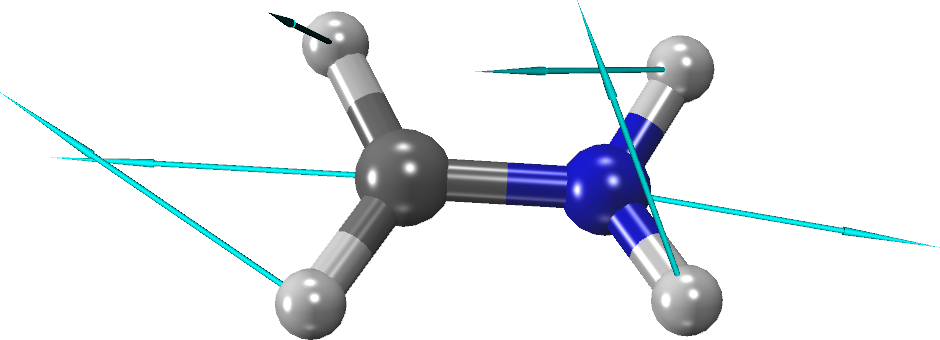
\includegraphics[width=0.7\textwidth]{figures/essdyn.png}
  \caption{Vector representation of the most active essential mode.}
  \label{fig:essdyn}
\end{figure}


% ======================================================================================================

\clearpage
\subsection{Normal Mode Analysis}
\refermanual{m-sec:trajana_nma.py}
\refermanual{m-met:nma}

An alternative to the essential dynamics analysis is a normal mode analysis.
The difference is that the essential dynamics analysis automatically identifies a suitable set of modes, whereas the normal mode analysis uses a set of precomputed normal modes (e.g., normal modes of the ground state minimum).

The interactive script can be started with 
\begin{Verbatim}[commandchars=\\\{\}]
user@host> \textbf{\textcolor{red}{$SHARC/trajana_nma.py}}
\end{Verbatim}

\begin{oframed}
\footnotesize\begin{Verbatim}[commandchars=\\\{\}]
  ================================================================================
||                                                                                ||
||                     Normal-mode analysis for SHARC dynamics                    ||
||                                                                                ||
||                      Author: Felix Plasser, Andrew Atkins                      ||
||                                                                                ||
||                                   Version:2.0                                  ||
||                                    01.02.18                                    ||
||                                                                                ||
  ================================================================================

This script reads output.xyz files, transforms into normal modes, and performs statistical analyses 
(i.e., Shows you which are the most important motions).
  
--------------------Paths to trajectories-------------------

Please enter the paths to all directories containing the "TRAJ_0XXXX" directories.
E.g. Sing_2/ and Sing_3/. 
Please enter one path at a time, and type "end" to finish the list.
Path:  [end] (autocomplete enabled) \textbf{\textcolor{red}{Singlet_2/}}
['TRAJ_00005', 'TRAJ_00004', 'TRAJ_00008', 'plot.gp', 'TRAJ_00009', 'TRAJ_00002', 
'TRAJ_00006', 'TRAJ_00010', 'TRAJ_00007', 'TRAJ_00003']
Found 9 subdirectories in total.

Path:  [end] (autocomplete enabled) \textbf{\textcolor{red}{<ENTER>}}

Total number of subdirectories: 9

------------------Path to normal mode file------------------

Please enter the path to the Molden normal mode file for your molecule. 
The contained geometry will be used as reference geometry.
(Atomic order must be the same as in the trajectories!)

Path:  (autocomplete enabled) \textbf{\textcolor{red}{../MOLCAS.freq.molden}}

Do you wish to use mass weighted normal modes? [True] \textbf{\textcolor{red}{<ENTER>}}

---------Number of total steps in your trajectories---------

Number of time steps:  [201] \textbf{\textcolor{red}{<ENTER>}}

--------------The time step of your calculation-------------

Length of time step:  [0.5] \textbf{\textcolor{red}{<ENTER>}}

-------------------Automatic plot creation------------------

Do you want to automatically create plots of your data? [False] \textbf{\textcolor{red}{yes}}

-------------Non-totally symmetric normal modes-------------

Please enter the numbers of the normal modes (numbering as in the Molden file) whose absolute 
value should be considered in the analysis. Without this setting, the average for all 
non-totally symmetric modes should be zero. Default is to not compute the absolute. 
Entering -1 ends this input section.

Non-totally symmetric normal modes: [-1] (range comprehension enabled) \textbf{\textcolor{red}{<ENTER>}}

--------------------Multiplication by -1--------------------
Please enter the numbers of normal modes whose values should be multiplied by -1 before 
statistical analysis (affects total_std.txt and cross_av_std.txt). This is only for convenience
when viewing the results. Entering -1 ends this input section.

Inverted normal modes: [-1] (range comprehension enabled) \textbf{\textcolor{red}{<ENTER>}}

------------------Time steps to be analysed-----------------

Please enter the time step intervals for which the statistical analysis should be carried out. 

Time step interval:  [0 200] \textbf{\textcolor{red}{<ENTER>}}

Do you want to add another time interval for analysis? [False] \textbf{\textcolor{red}{<ENTER>}}

----------------------Results directory---------------------
Please give the name of the subdirectory to be used for the results (use to save similar 
analysis in separate subdirectories).
Name for subdirectory? [nma] (autocomplete enabled) \textbf{\textcolor{red}{<ENTER>}}

Preparing NMA ...
Checking the directories...
Singlet_2//TRAJ_00005         OK
Singlet_2//TRAJ_00004         OK
Singlet_2//TRAJ_00008         OK
Singlet_2//TRAJ_00009         DETECTED FILE dont_analyze
Singlet_2//TRAJ_00002         OK
Singlet_2//TRAJ_00006         OK
Singlet_2//TRAJ_00010         DETECTED FILE dont_analyze
Singlet_2//TRAJ_00007         OK
Singlet_2//TRAJ_00003         OK
Number of trajectories: 7
Reading trajectory Singlet_2//TRAJ_00005/output.xyz ...
Reading trajectory Singlet_2//TRAJ_00004/output.xyz ...
Reading trajectory Singlet_2//TRAJ_00008/output.xyz ...
Reading trajectory Singlet_2//TRAJ_00002/output.xyz ...
Reading trajectory Singlet_2//TRAJ_00006/output.xyz ...
Reading trajectory Singlet_2//TRAJ_00007/output.xyz ...
Reading trajectory Singlet_2//TRAJ_00003/output.xyz ...
Processing data ...
Data processing finished.
Drawing plots ...
\end{Verbatim}
\end{oframed}

\normalsize
The output of this script is a directory \ttt{NMA/nma/}, which contains four output files, \ttt{mean\_against\_time.txt} and \ttt{std\_against\_time.txt}, \ttt{total\_std.txt}, and \ttt{cross\_av\_std.txt}.
The content of the first two files is plotted in subdirectory \ttt{time\_plots/}, whereas the content of the two other files is plotted in subdirectory \ttt{bar\_graphs/}.

The file  \ttt{NMA/nma/bar\_graphs/total\_std/0-200.png} is plotted in Figure~\ref{fig:nma}.
It shows that the most active mode is mode~8, which is the \ce{C=N} stretch mode, followed by modes 6 and 7, which are the \ce{H-C-H} and \ce{H-N-H} bend modes.

Note that \ttt{trajana\_nma.py} also produces output files in all trajectory folders.
These files contain the coordinates of the trajectory converted to normal mode coordinates (complementary to output of \ttt{geo.py}).

\begin{figure}[ptb]
  \centering
  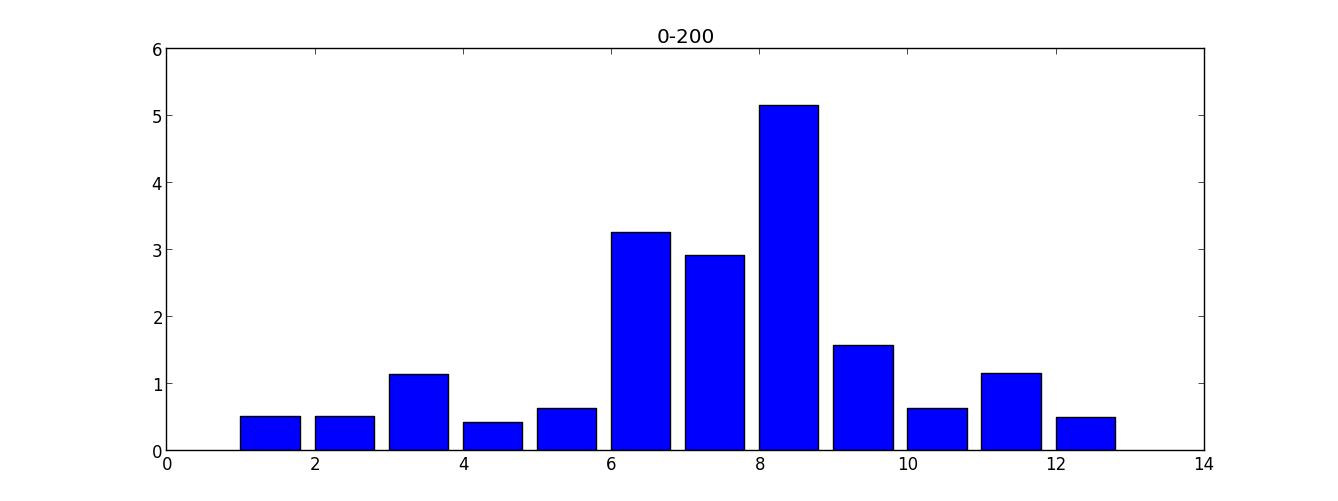
\includegraphics[width=0.7\textwidth]{figures/nma.png}
  \caption{Total activity of the normal modes of \ce{CH2NH2+}, where modes 6, 7, and 8 show the highest activity.}
  \label{fig:nma}
\end{figure}




% ======================================================================================================

\clearpage
\subsection{Ensemble Motion Plots}
\refermanual{m-sec:data_collector.py}

In addition to the statistical analysis of the nuclear motion (\ttt{trajana\_essdyn.py} and \ttt{trajana\_nma.py}), it is often helpful to plot some bond length, angle, internal coordinate, etc.\ for all trajectories, in what could be called ``hair figures'' or heat maps.
For such plots (and many others), \ttt{data\_collector.py} can merge the corresponding per-trajectory data into files which can then be conveniently plotted.

In the following, we will collect the time-dependent \ce{C=N} bond length from all trajectories and plot them.
The first step is to compute this bond length for each trajectory.
This can be achieved with \ttt{geo.py} and a simple Bash loop:
\begin{Verbatim}[commandchars=\\\{\}]
user@host> \textbf{\textcolor{red}{echo "r 1 2" > Geo.inp}}
user@host> \textbf{\textcolor{red}{for i in Singlet_2/TRAJ_000*;}}
user@host> \textbf{\textcolor{red}{$SHARC/geo.py -t 0.5 -g $i/output.xyz < Geo.inp > $i/Geo.out;}}
user@host> \textbf{\textcolor{red}{done}}
\end{Verbatim}
This will create a file \ttt{Geo.out} for each trajectory with the bond length between atoms 1 and 2.

Then, start the \ttt{data\_collector.py} to merge the data into a single file (note that the excluded trajectories are ignored):
\begin{Verbatim}[commandchars=\\\{\}]
user@host> \textbf{\textcolor{red}{$SHARC/data_collector.py}}
\end{Verbatim}

\begin{oframed}
\footnotesize\begin{Verbatim}[commandchars=\\\{\}]
  ================================================================================
||                                                                                ||
||                     Reading table data from SHARC dynamics                     ||
||                                                                                ||
||                              Author: Sebastian Mai                             ||
||                                                                                ||
||                                   Version:2.0                                  ||
||                                    01.02.18                                    ||
||                                                                                ||
  ================================================================================


This script collects table data from SHARC trajectories, smooths them, synchronizes them,
convolutes them, and computes averages and similar statistics.
  
--------------------Paths to trajectories-------------------

Please enter the paths to all directories containing the "TRAJ_0XXXX" directories.
E.g. Sing_2/ and Sing_3/. 
Please enter one path at a time, and type "end" to finish the list.
Path:  [end] (autocomplete enabled) \textbf{\textcolor{red}{Singlet_2/}}
['TRAJ_00005', 'TRAJ_00004', 'TRAJ_00008', 'plot.gp', 'TRAJ_00009', 'TRAJ_00002',
'TRAJ_00006', 'TRAJ_00010', 'TRAJ_00007', 'TRAJ_00003']
Found 9 subdirectories in total.

Path:  [end] (autocomplete enabled) \textbf{\textcolor{red}{<ENTER>}}

Total number of subdirectories: 9

Checking the directories...
Number of trajectories: 7
Checking for common files...

List of files common to the trajectory directories:

 Index Number of appearance   Relative file path
----------------------------------------------------------
     0                    7   ./Geo.out
     1                    7   ./nma_nma.txt
     2                    7   ./nma_nma_av.txt
     3                    7   ./nma_nma_std.txt
     4                    7   ./output.lis
     5                    7   output_data/coeff_MCH.out
     6                    7   output_data/coeff_diab.out
     7                    7   output_data/coeff_diag.out
     8                    7   output_data/energy.out
     9                    7   output_data/expec.out
    10                    7   output_data/expec_MCH.out
    11                    7   output_data/fosc.out
    12                    7   output_data/fosc_act.out
    13                    7   output_data/prob.out
    14                    7   output_data/spin.out

Please give the relative file path of the file you want to collect:
File path or index: [0] \textbf{\textcolor{red}{./Geo.out}}

------------------------Data columns------------------------

Number of columns in the file:   2

Please select the data columns for the analysis:
For T column: 
  only enter one (positive) column index. 
  If 0, the line number will be used instead.
For X column: 
  enter one or more column indices. 
  If 0, all entries of that column will be set to 1. 
  If negative, the read numbers will be multiplied by -1.
For Y column: 
  enter as many column indices as for X. 
  If 0, all entries of that column will be set to 1. 
  If negative, the read numbers will be multiplied by -1.

T column (time): [1] \textbf{\textcolor{red}{<ENTER>}}
X columns: [2] (range comprehension enabled) \textbf{\textcolor{red}{<ENTER>}}
Y columns: [0] (range comprehension enabled) \textbf{\textcolor{red}{<ENTER>}}
Selected columns:
T: 1     X: [2]    Y: [0]

---------------------Analysis procedure---------------------

Show possible workflow options? [True] \textbf{\textcolor{red}{no}}

---------------1 Smoothing--------------

Do you want to apply smoothing to the individual trajectories? [False] \textbf{\textcolor{red}{<ENTER>}}

-------------2 Synchronizing------------

Do you want to synchronize the data? [True] \textbf{\textcolor{red}{<ENTER>}}


----------3 Convoluting along X---------

Do you want to apply convolution in X direction? [False] \textbf{\textcolor{red}{yes}}

Choose one of the following convolution kernels:
1  Gaussian function
2  Lorentzian function
3  Rectangular window function
4  Log-normal function
Choose one of the functions: [1] \textbf{\textcolor{red}{<ENTER>}}
Choose width of the smoothing function (in units of the X columns): [1.0] \textbf{\textcolor{red}{0.2}}
Size of the grid along X: [25] \textbf{\textcolor{red}{50}}

Choose minimum and maximum of the grid along X:
Enter either a single number a (X grid from  xmin-a*width  to  xmax+a*width)
        or two numbers a and b (X grid from  a  to  b)
Xrange: [1.5] \textbf{\textcolor{red}{<ENTER>}}

------------6 Sum over all Y------------

Do you want to sum up all Y values? [False] \textbf{\textcolor{red}{<ENTER>}}

-----------7 Integrate along X----------

Do you want to integrate in X direction? [False] \textbf{\textcolor{red}{<ENTER>}}

----------8 Convoluting along T---------

Do you want to apply convolution in T direction? [False] \textbf{\textcolor{red}{<ENTER>}}

----------9 Integrating along T---------

Do you want to integrate in T direction? [False] \textbf{\textcolor{red}{<ENTER>}}

-------10 Convert to Type2 dataset------

If you performed integration along X, the data might be better formatted as Type2 dataset.
Do you want to output as Type2 dataset? [False] \textbf{\textcolor{red}{<ENTER>}}


#########################Full input#########################

paths                      ['Singlet_2/']
statistics                 \{\}
allfiles                   ['Singlet_2//TRAJ_00002/./Geo.out', 
                            'Singlet_2//TRAJ_00003/./Geo.out', 
                            'Singlet_2//TRAJ_00004/./Geo.out', 
                            'Singlet_2//TRAJ_00005/./Geo.out', 
                            'Singlet_2//TRAJ_00006/./Geo.out', 
                            'Singlet_2//TRAJ_00007/./Geo.out', 
                            'Singlet_2//TRAJ_00008/./Geo.out']
colX                       [2]
filepath                   ./Geo.out
averaging                  \{\}
colT                       1
colY                       [0]
synchronizing              True
smoothing                  \{\}
nX                         1
nY                         1
convolute_T                \{\}
ncol                       2
type3_to_type2             False
integrate_X                \{\}
sum_Y                      False
integrate_T                False
convolute_X                \{'function': <__main__.gauss instance at 0x1a7ed88>, 
                            'npoints': 50, 'xrange': [1.5]\}

Do you want to do the specified analysis? [True] \textbf{\textcolor{red}{<ENTER>}}

>>>>>>>>>>>>>>>>>>>>>> Started data analysis

Collecting the data ...
  Progress: [==================================================] 100%
>>>> Writing output to file "collected_data_1_2_0.type1.txt"...

Synchronizing temporal data ...
  Progress: [==================================================] 100%
>>>> Writing output to file "collected_data_1_2_0_sy.type2.txt"...

Convoluting data (along X column) ...
  Progress: [==================================================] 100%
>>>> Writing output to file "collected_data_1_2_0_sy_cX.type3.txt"...
\end{Verbatim}
\end{oframed}

\normalsize
This run of the script produces three output files:
\begin{itemize}
  \item \ttt{collected\_data\_1\_2\_0.type1.txt},
  \item \ttt{collected\_data\_1\_2\_0\_sy.type2.txt}, and
  \item \ttt{collected\_data\_1\_2\_0\_sy\_cX.type3.txt}.
\end{itemize}
You can plot the contained data using \textsc{Gnuplot} (do not type the line break):
\begin{Verbatim}[commandchars=\\\{\}]
gnuplot> \textbf{\textcolor{red}{p "collected_data_1_2_0_sy.type2.txt" u 1:2 w l, "" u 1:3 w l,}}
         \textbf{\textcolor{red}{"" u 1:4 w l, "" u 1:5 w l, "" u 1:6 w l, "" u 1:7 w l, "" u 1:8 w l}}
\end{Verbatim}
or (if using \textsc{Gnuplot} 5.0 or higher):
\begin{Verbatim}[commandchars=\\\{\}]
gnuplot> \textbf{\textcolor{red}{p for [col=2:8] "collected_data_1_2_0_sy.type2.txt" u 1:col w l}}
\end{Verbatim}
For the 3D data in \ttt{collected\_data\_1\_2\_0\_sy\_cX.type3.txt}, use:
\begin{Verbatim}[commandchars=\\\{\}]
gnuplot> \textbf{\textcolor{red}{set view map}}
gnuplot> \textbf{\textcolor{red}{sp "collected_data_1_2_0_sy_cX.type3.txt" u 1:2:3 w pm3d}}
\end{Verbatim}
The results of these two plot commands are shown in Figures~\ref{fig:coll_1_2} and \ref{fig:coll_1_2_cX}.

Using \ttt{data\_collector.py}, it is also possible to compute the mean and standard deviations of the bond lengths (giving similar information as \ttt{trajana\_nma.py} was doing for the normal modes).
In order to do so, do not apply convolution in X direction, and then ask for an averaging and/or statistics analysis.


\begin{figure}[p]
  \centering
  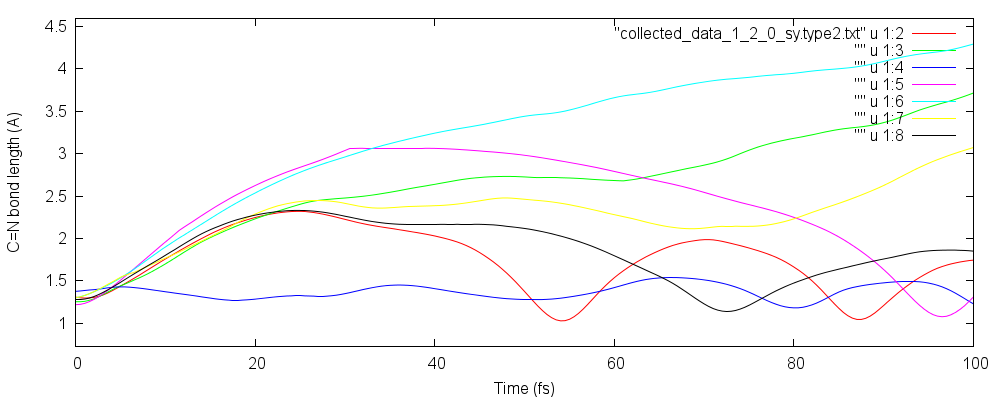
\includegraphics[width=0.7\textwidth]{figures/coll_1_2.png}
  \caption{All \ce{C=N} bond lengths from the 7 trajectories.}
  \label{fig:coll_1_2}
\end{figure}

\begin{figure}[p]
  \centering
  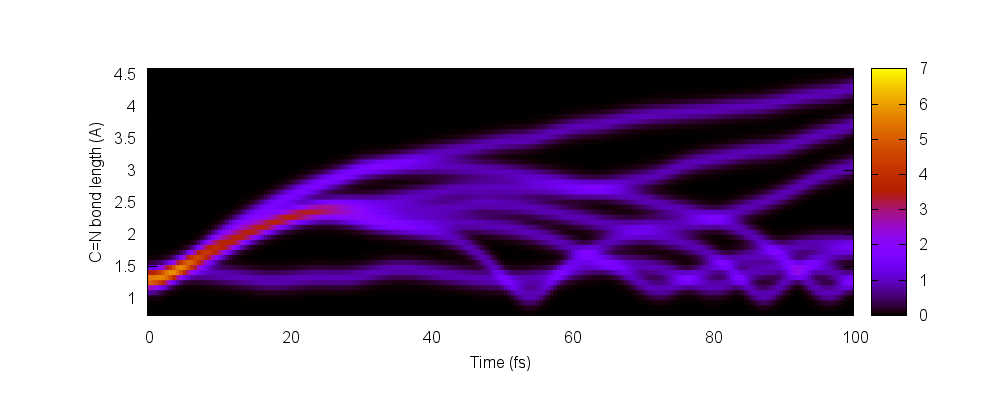
\includegraphics[width=0.7\textwidth]{figures/coll_1_2_cX.png}
  \caption{Convolution of the \ce{C=N} bond lengths from the 7 trajectories.}
  \label{fig:coll_1_2_cX}
\end{figure}











% ======================================================================================================

\clearpage
\subsection{Transient Spectra}
\refermanual{m-sec:data_collector.py}

Using \ttt{data\_collector.py}, it is also possible to compute transient absorption spectra, given that enough states were included in the simulations.
Here, we will simulate the transient spectrum for \ce{CH2NH2+}, although probably the spectrum will be incomplete due to the missing of higher excited states.

Again, start the \ttt{data\_collector.py} to merge and post-process the data:
\begin{Verbatim}[commandchars=\\\{\}]
user@host> \textbf{\textcolor{red}{$SHARC/data_collector.py}}
\end{Verbatim}

\begin{oframed}
\footnotesize\begin{Verbatim}[commandchars=\\\{\}]
  ================================================================================
||                                                                                ||
||                     Reading table data from SHARC dynamics                     ||
||                                                                                ||
||                              Author: Sebastian Mai                             ||
||                                                                                ||
||                                   Version:2.0                                  ||
||                                    01.02.18                                    ||
||                                                                                ||
  ================================================================================


This script collects table data from SHARC trajectories, smooths them, synchronizes them,
convolutes them, and computes averages and similar statistics.
  
--------------------Paths to trajectories-------------------

Please enter the paths to all directories containing the "TRAJ_0XXXX" directories.
E.g. Sing_2/ and Sing_3/. 
Please enter one path at a time, and type "end" to finish the list.
Path:  [end] (autocomplete enabled) \textbf{\textcolor{red}{Singlet_2/}}
['TRAJ_00005', 'TRAJ_00004', 'TRAJ_00008', 'plot.gp', 'TRAJ_00009', 'TRAJ_00002', 
'TRAJ_00006', 'TRAJ_00010', 'TRAJ_00007', 'TRAJ_00003']
Found 9 subdirectories in total.

Path:  [end] (autocomplete enabled) \textbf{\textcolor{red}{<ENTER>}}

Total number of subdirectories: 9

Checking the directories...
Number of trajectories: 7
Checking for common files...

List of files common to the trajectory directories:

 Index Number of appearance   Relative file path
----------------------------------------------------------
     0                    7   ./Geo.out
     1                    7   ./nma_nma.txt
     2                    7   ./nma_nma_av.txt
     3                    7   ./nma_nma_std.txt
     4                    7   ./output.lis
     5                    7   output_data/coeff_MCH.out
     6                    7   output_data/coeff_diab.out
     7                    7   output_data/coeff_diag.out
     8                    7   output_data/energy.out
     9                    7   output_data/expec.out
    10                    7   output_data/expec_MCH.out
    11                    7   output_data/fosc.out
    12                    7   output_data/fosc_act.out
    13                    7   output_data/prob.out
    14                    7   output_data/spin.out

Please give the relative file path of the file you want to collect:
File path or index: [0] \textbf{\textcolor{red}{output_data/fosc_act.out}}

------------------------Data columns------------------------

Number of columns in the file:   27

Please select the data columns for the analysis:
For T column: 
  only enter one (positive) column index. 
  If 0, the line number will be used instead.
For X column: 
  enter one or more column indices. 
  If 0, all entries of that column will be set to 1. 
  If negative, the read numbers will be multiplied by -1.
For Y column: 
  enter as many column indices as for X. 
  If 0, all entries of that column will be set to 1. 
  If negative, the read numbers will be multiplied by -1.

T column (time): [1] \textbf{\textcolor{red}{<ENTER>}}
X columns: [2] (range comprehension enabled) \textbf{\textcolor{red}{2~14}}
Y columns: [0 0 0 0 0 0 0 0 0 0 0 0 0] (range comprehension enabled) \textbf{\textcolor{red}{15~27}}
Selected columns:
T: 1     X: [2, 3, 4, 5, 6, 7, 8, 9, 10, 11, 12, 13, 14]    
         Y: [15, 16, 17, 18, 19, 20, 21, 22, 23, 24, 25, 26, 27]

---------------------Analysis procedure---------------------

Show possible workflow options? [True] \textbf{\textcolor{red}{no}}

---------------1 Smoothing--------------

Do you want to apply smoothing to the individual trajectories? [False] \textbf{\textcolor{red}{<ENTER>}}

-------------2 Synchronizing------------

Do you want to synchronize the data? [True] \textbf{\textcolor{red}{<ENTER>}}

----------3 Convoluting along X---------

Do you want to apply convolution in X direction? [False] \textbf{\textcolor{red}{yes}}

Choose one of the following convolution kernels:
1  Gaussian function
2  Lorentzian function
3  Rectangular window function
4  Log-normal function
Choose one of the functions: [1] \textbf{\textcolor{red}{<ENTER>}}
Choose width of the smoothing function (in units of the X columns): [1.0] \textbf{\textcolor{red}{<ENTER>}}
Size of the grid along X: [25] \textbf{\textcolor{red}{50}}

Choose minimum and maximum of the grid along X:
Enter either a single number a (X grid from  xmin-a*width  to  xmax+a*width)
        or two numbers a and b (X grid from  a  to  b)
Xrange: [1.5] \textbf{\textcolor{red}{<ENTER>}}

------------6 Sum over all Y------------

Do you want to sum up all Y values? [False] \textbf{\textcolor{red}{yes}}

-----------7 Integrate along X----------

Do you want to integrate in X direction? [False] \textbf{\textcolor{red}{<ENTER>}}

----------8 Convoluting along T---------

Do you want to apply convolution in T direction? [False] \textbf{\textcolor{red}{<ENTER>}}

----------9 Integrating along T---------

Do you want to integrate in T direction? [False] \textbf{\textcolor{red}{<ENTER>}}

-------10 Convert to Type2 dataset------

If you performed integration along X, the data might be better formatted as Type2 dataset.
Do you want to output as Type2 dataset? [False] \textbf{\textcolor{red}{<ENTER>}}


#########################Full input#########################

paths                      ['Singlet_2/']
statistics                 \{\}
allfiles                   ['Singlet_2//TRAJ_00002/output_data/fosc_act.out',
                            'Singlet_2//TRAJ_00003/output_data/fosc_act.out',
                            'Singlet_2//TRAJ_00004/output_data/fosc_act.out',
                            'Singlet_2//TRAJ_00005/output_data/fosc_act.out',
                            'Singlet_2//TRAJ_00006/output_data/fosc_act.out',
                            'Singlet_2//TRAJ_00007/output_data/fosc_act.out',
                            'Singlet_2//TRAJ_00008/output_data/fosc_act.out']
colX                       [2, 3, 4, 5, 6, 7, 8, 9, 10, 11, 12, 13, 14]
filepath                   output_data/fosc_act.out
averaging                  \{\}
colT                       1
colY                       [15, 16, 17, 18, 19, 20, 21, 22, 23, 24, 25, 26, 27]
synchronizing              True
smoothing                  \{\}
nX                         13
nY                         13
convolute_T                \{\}
ncol                       27
type3_to_type2             False
integrate_X                \{\}
sum_Y                      True
integrate_T                False
convolute_X                \{'function': <__main__.gauss instance at 0x28e0c20>, 
                            'npoints': 50, 'xrange': [1.5]\}

Do you want to do the specified analysis? [True] \textbf{\textcolor{red}{<ENTER>}}



>>>>>>>>>>>>>>>>>>>>>> Started data analysis

Collecting the data ...
  Progress: [==================================================] 100%
>>>> Writing output to "collected_data_1_234567891011121314_15161718192021222324252627.type1.txt"...

Synchronizing temporal data ...
  Progress: [==================================================] 100%
>>>> Writing output to "collected_data_1_234567891011121314_15161718192021222324252627_sy.type2.txt"...

Convoluting data (along X column) ...
  Progress: [==================================================] 100%
>>>> Writing output to "collected_data_1_234567891011121314_15161718192021222324252627_sy_cX.type3.txt"...

Summing all Y values ...
  Progress: [==================================================] 100%
>>>> Writing output to "collected_data_1_234567891011121314_15161718192021222324252627_sy_cX_sY.type3.txt"...

\end{Verbatim}
\end{oframed}

\normalsize
The last of the four produced output files contains the total transient absorption spectrum.
You can print it in the same way as the convoluted bond lengths in Figure~\ref{fig:coll_1_2_cX}.
The simulated transient absorption spectrum is presented in Figure~\ref{fig:TAS}.

Using \ttt{data\_collector.py}, it is also possible to convolute the spectrum with an instrument response function, or to integrate it along the time or energy axes.

\begin{figure}[h]
  \centering
  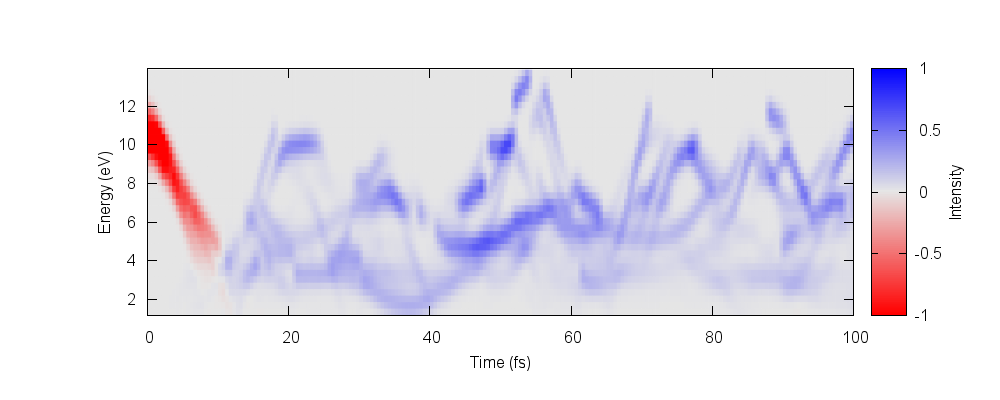
\includegraphics[width=0.9\textwidth]{figures/TAS.png}
  \caption{Simulated transient absorption spectrum of \ce{CH2NH2+}. Ground state bleech (negative absorption) is shown in red, and excited-state absorption (positive absorption) is shown in blue.}
  \label{fig:TAS}
\end{figure}








% ======================================================================================================
% ======================================================================================================
% ======================================================================================================

\chapter{Specialized Tutorials}

This chapter collects some more tutorials on advanced aspects of the \sharc\ suite.
In order to keep this chapter short and simple, not the full input dialogues are shown, but only the relevant parts.
It is thus a good idea to first work through the full tutorial in Chapter~\ref{chap:full}.

\section{Using non-default atomic masses}

Sometimes, in dynamics simulations one is interested in isotope effects. This necessitates the modification of the atomic mass of the corresponding atoms. The atomic masses are included in the geometry file, which is read by \sharc\ during initialization of the dynamics.

Furthermore, modification of the atomic masses influences the Wigner distribution of initial conditions. \ttt{wigner.py} has a facility to adjust the atomic mass during initial condition generation. Call \ttt{wigner.py} as usual, but include the \ttt{-m} option:
\begin{Verbatim}[commandchars=\\\{\}]
user@host> \textbf{\textcolor{red}{$SHARC/wigner.py freq.molden -m}}
\end{Verbatim}

Instead of directly producing the initial conditions file, \ttt{wigner.py} will start a dialog, where the user can modify the atomic masses. Initially, all atoms are assumed to use the default mass (the mass of the most common isotope). The user can then add atoms to the list of atoms with non-default masses, thereby specifying the mass. 
\begin{oframed}
\footnotesize\begin{Verbatim}[commandchars=\\\{\}]
Initial condition generation started...
\textsc{Molden} file                  = "MOLCAS.freq.molden"
OUTPUT file                  = "initconds"
Number of geometries         = 20
Random number generator seed = 16661
Temperature                  = 0.000000

Option -m used, please enter non-default masses:
+ number mass           add non-default mass <mass> for atom <number>
- number                remove non-default mass for atom <number> (default mass will be used)
show                    show non-default atom masses
end                     finish input for non-default masses

\textbf{\textcolor{red}{+ 1 14.054321}}         \textcolor{blue}{# Give atom number 1 the mass 14.054321}
\textbf{\textcolor{red}{show}}
-----------------------
Atom               Mass
   1    14.054321000000
-----------------------
\textbf{\textcolor{red}{- 1}}                   \textcolor{blue}{# Give atom number 1 the default mass}
\textbf{\textcolor{red}{+ 2 16.054321}}         \textcolor{blue}{# Give atom number 2 the mass 16.054321}
\textbf{\textcolor{red}{+ 2 15.054321}}         \textcolor{blue}{# Give atom number 2 the mass 15.054321}
\textbf{\textcolor{red}{end}}
***************************************************
WARNING: Less than 3*N_atom normal modes extracted!
***************************************************


Starting normal mode format determination...
Final format specifier: 2 [cartesian (Molpro, Molcas)]
Multiple possible flags have been identified: 
  gaussian-type (Gaussian, Turbomole, Q-Chem, ADF, Orca) 
  cartesian (Molpro, Molcas)
The most likely assumption is cartesian (Molpro, Molcas) coordinates.
These have been used in the creation of inital conditions.

You can override this behavior by setting the -f [int] flag in the command line:
  1     gaussian-type (Gaussian, Turbomole, Q-Chem, ADF, Orca)
  2     cartesian (Molpro, Molcas)
  3     columbus-type (Columbus)
  4     mass-weighted

Geometry:
 C   6.0   0.00000000  -0.00000000   0.06174827  12.00000000 
 N   7.0   0.00000000  -0.00000000   2.46709935  15.05432100 
 H   1.0   1.77794247  -0.00000014  -0.94890055   1.00782000 
 H   1.0   1.62604543   0.00000016   3.46865331   1.00782000 
 H   1.0  -1.62604543  -0.00000016   3.46865331   1.00782000 
 H   1.0  -1.77794247   0.00000014  -0.94890055   1.00782000 
Assumed Isotopes: H-1 C-12 N-14 
Isotopes with * are pure isotopes.

Frequencies (cm^-1) used in the calculation:
   1     977.8746
   2    1022.0225
   3    1215.0055
   4    1314.4262
   5    1418.2342
   6    1537.7263
   7    1679.1657
   8    1882.6738
   9    3329.5794
  10    3463.0910
  11    3679.5594
  12    3763.5119

Sampling initial conditions
Progress: [==================================================] 100%
\end{Verbatim}
\end{oframed}

\normalsize
Note that with the \ttt{+} command the mass of an already specified atom can also be changed. 

\paragraph{Frequency calculation}

Please also note that the preceding frequency calculation also has to use the same atomic masses as the run of \ttt{wigner.py}. 
For \textsc{Molcas}, after running \ttt{molcas\_input.py} it will be necessary to adjust the input file by adding the appropriate keywords (consult the \textsc{Molcas} manual).
For \textsc{Molpro}, \ttt{molpro\_input.py} can setup frequency calculations with non-standard atomic masses. 
For \textsc{Columbus}, the user can edit the \ttt{geom} before starting the frequency calculation.



% ======================================================================================================

\section{Inactive states}

Sometimes, states should be included in the dynamics simulation in order to calculate transient absorption spectra, transient ionization spectra or simply in order to see how these states evolve during the dynamics. When it is not expected that these states are actually occupied during the simulation, \sharc\ has a mechanism to neglect all couplings between these states (called inactive henceforth) and the occupied states. This allows also to neglect the gradients and non-adiabatic couplings involving these states, thereby saving considerable amounts of computation time. 

It is only possible to make the highest states in each multiplicity inactive. With \ttt{states 3 0 3} and \ttt{actstates 2 0 1} in the \sharc\ input, one would include $S_0$, $S_1$, $S_2$, $T_1$, $T_2$ and $T_3$ in the simulation, but restrict the actual dynamics to $S_0$, $S_1$ and $T_1$.
This is useful, e.g., to compute a transient absorption spectrum involving the higher states.

It is advisable to make inactive all states which do not show any couplings with the occupied states (e.g., ionic states in a dynamics simulation of a neutral molecule). 

\paragraph{Inactive states in \ttt{excite.py}}

\ttt{excite.py} also allows to exclude states in the excitation process. Note, however, that this is unrelated to the inactive states in the dynamics. It would be possible to exclude a state in the excitation process but still keep it in the dynamics simulation. An example would be to excite to dark $n\pi^*$ states, which would not be selected if bright $\pi\pi^*$ states are present.



% ======================================================================================================

\section{Ionization spectra}
\refermanual{m-sec:setup_init.py}
\refermanual{m-sec:excite.py}
\refermanual{m-sec:int:overview}

With some of the \sharc\ interfaces, it is possible to compute Dyson norms between pairs of neutral and ionic states. These Dyson norms are very simple estimates for the single-photon ionization probability, and therefore allow to compute approximate ionization spectra. 

In order to compute ionization spectra, one needs first to prepare an \ttt{initconds} file, e.g., using \ttt{wigner.py}.
Subsequently, one uses \ttt{setup\_init.py} to setup the necessary single point calculations, \ttt{excite.py} to read out the resulting data, and \ttt{spectrum.py} to plot the ionization spectrum.

In order to prepare the computation (assuming you did the full tutorial beforehand):
\begin{Verbatim}[commandchars=\\\{\}]
user@host> \textbf{\textcolor{red}{mkdir ionization}}
user@host> \textbf{\textcolor{red}{cp MOLCAS.template initconds ionization/}}
user@host> \textbf{\textcolor{red}{cd ionization/}}
\end{Verbatim}
Then, modify \ttt{MOLCAS.template} by setting the number of states for averaging to \ttt{roots 4 3 3} and the number of electrons to \ttt{nactel 7}. The other settings (basis set, RAS2, inactive) should stay the same as in the full tutorial (\ttt{basis cc-pVDZ}, \ttt{ras2 4}, \ttt{inactive 5}).
With this setup, the interface will do the odd multiplicities (doublets) with CAS(7,4) and the even multiplicities (singlets, triplets) with CAS(6,4), because the interface will always either use the given \ttt{nactel} or \ttt{nactel}$-1$, as appropriate.

\subsection{\ttt{setup\_init.py} Input}

Carry out the \ttt{setup\_init.py} input dialogue as usual, but request \ttt{4 3 3} states and then the computation of Dyson norms:
\begin{oframed}
\footnotesize\begin{Verbatim}[commandchars=\\\{\}]
----------------------Number of states----------------------

Please enter the number of states as a list of integers
e.g. 3 0 3 for three singlets, zero doublets and three triplets.
Number of states: \textbf{\textcolor{red}{4  3  3}}

Number of states: [4, 3, 3]
Total number of states: 19

\vdots   \vdots   \vdots   \vdots   \vdots   \vdots   \vdots   \vdots   

------------Ionization probability by Dyson norms-----------

Do you want to compute Dyson norms between neutral and ionic states?
Dyson norms? [False] \textbf{\textcolor{red}{yes}}
\end{Verbatim}
\end{oframed}

\normalsize
The latter question is only asked if you requested doublet states and the interface can compute Dyson norms (which the \textsc{Molcas} interface can).
Finish the setup as usual and run the calculations.

\subsection{\ttt{excite.py} Input}

Use \ttt{excite.py} as usual to read the results of the excited-state calculations. 
Tell the script to consider the Dyson norms instead of the transition dipole moments, and tell it to assume excitation from state 5 (with \ttt{states 4 3 3}, state 5 is the lowest doublet state). 
\begin{oframed}
\footnotesize\begin{Verbatim}[commandchars=\\\{\}]
Use Dyson norms instead of dipole moments? [False] \textbf{\textcolor{red}{yes}}

\vdots   \vdots   \vdots   \vdots   \vdots   \vdots   \vdots   \vdots   

----------------------Considered states---------------------

From which state should the excitation originate (for computation of excitation energies 
and oscillator strength)?
Lower state for excitation? [1] \textbf{\textcolor{red}{5}}
\end{Verbatim}
\end{oframed}

\normalsize
The script will use the Dyson norms in the place of the $x$ component of the transition dipole moments, while the $y$ and $z$ components will be set to zero. The remaining usage is identical to the regular case (transition dipole moments). \ttt{spectrum.py} can be used to obtain plottable spectra.


% ======================================================================================================

\section{Initial Conditions from Dynamics Simulations}
\refermanual{m-sec:sharctraj_to_initconds.py}
\refermanual{m-sec:amber_to_initconds.py}

Instead of generating the initial geometries/velocities with \ttt{wigner.py}, one can sample them from a molecular dynamics simulation (usually in the ground state).
Within \sharc, there are two possibilities: (i) convert \sharc\ trajectories, (ii) convert \textsc{Amber} restart files.
The first option is described below, for the second option, please refer to the Manual.

\subsection{Converting \sharc\ Trajectories}

In order to convert \sharc\ trajectories back into an \ttt{initconds} file, use the script \ttt{sharctraj\_to\_initconds.py}.
Here, we will convert the trajectories ran within the full tutorial (chapter~\ref{chap:full}).
More specifically, we will take the geometry from a random time step which is later than the first 100 steps (because in the beginning the system needs to relax), and earlier than the last 20 steps (because the last time step might be a crash and we do not want to start the new simulations at the related geometry).

This can be done with the following (assuming you are in the \ttt{traj/} directory):
\begin{oframed}
\footnotesize\begin{Verbatim}[commandchars=\\\{\}]
user@host> \textbf{\textcolor{red}{$SHARC/sharctraj_to_initconds.py -S 100 -20 -o initconds_II Singlet_2/}}
Initial condition generation started...
directories                    = "['Singlet_2/']"
Random number generator seed   = 16661
Pick randomly from these steps = 100 to -20  (negative indices are counted from the end)
OUTPUT file                    = "initconds_II"
Structure     0: Singlet_2/TRAJ_00002/output.dat  Step:   178/  200  (Reference geometry)
Structure     1: Singlet_2/TRAJ_00002/output.dat  Step:   131/  200  (Saved for initconds)
Structure     2: Singlet_2/TRAJ_00003/output.dat  Step:   150/  200  (Saved for initconds)
Structure     3: Singlet_2/TRAJ_00004/output.dat  Step:   169/  200  (Saved for initconds)
Structure     4: Singlet_2/TRAJ_00005/output.dat  Step:   116/  200  (Saved for initconds)
Structure     5: Singlet_2/TRAJ_00006/output.dat  Step:   181/  200  (Saved for initconds)
Structure     6: Singlet_2/TRAJ_00007/output.dat  Step:   143/  200  (Saved for initconds)
Structure     7: Singlet_2/TRAJ_00008/output.dat  Step:   109/  200  (Saved for initconds)
\end{Verbatim}
\end{oframed}

\normalsize
The script will then proceed to check the trajectories.
Those marked with files \ttt{CRASHED}, or \ttt{DONT\_ANALYZE} will be ignored (like in all analysis scripts).
The other trajectories are all 200 steps long, and therefore the script picks in the time step range 100--180.
Each trajectory will give rise to one new initial condition, with the exception that the first trajectory will also be used to create the reference geometry (this is not a real equilibrium geometry, but the \ttt{initconds} file format requires some reference geometry).
In the end, the script will write the file \ttt{initconds\_II} (according to the \ttt{-o} option), which can be used to compute spectra or setup new trajectories.



% ======================================================================================================

\section{Setting up Laser Fields}
\refermanual{m-sec:laser.x}
\refermanual{m-met:laser_field}

In order to generate a laser field file for a \sharc\ simulation driven by a laser field, one can use the program \ttt{laser.x}.
\begin{Verbatim}[commandchars=\\\{\}]
user@host> \textbf{\textcolor{red}{$SHARC/laser.x}}
\end{Verbatim}

In this example, a short Gaussian laser pulse is set up, using a central wave length of 112~nm (equivalent to 11~eV, the excitation energy of \ce{CH2NH2+} with the method used in the full tutorial (chapter~\ref{chap:full}).
The laser file is prepared for a 100~fs long \sharc\ simulation with 0.5~fs step and 25 substeps per step (giving 100~fs/0.5~fs*25+1=5001 steps).
\begin{oframed}
\footnotesize\begin{Verbatim}[commandchars=\\\{\}]
 Number of lasers:
\textbf{\textcolor{red}{1}}
           1
 Real-valued field (T) or not (F):
\textbf{\textcolor{red}{T}}
 T
 Set starting time, end of time and number of time steps (t0[fs],tEnd[fs],Nt) :
\textbf{\textcolor{red}{0 100 5001}}          \textcolor{blue}{# one step for each substep in sharc.x}
  0.000000000000000E+000   100.000000000000             5001
 consequently, we have a step size of   2.000000000000000E-002
 Write additional files for debugging (T) or not (F):
\textbf{\textcolor{red}{F}}
 F
              (Empty line to increase readability. Press Enter.)
\textbf{\textcolor{red}{<ENTER>}}
 
 Choose polarization vector (e.g. 2.,0.,0. will be normalized):
\textbf{\textcolor{red}{0 0 1}}         \textcolor{blue}{# orientation of transition dipole moment of CH2NH2+}
  0.000000000000000E+000  0.000000000000000E+000   1.00000000000000     
 Choose type of envelope (1=Gaussian,2=Sinusoidal):
\textbf{\textcolor{red}{1}}
           1
 Choose field strength in (1) [GV/m] (2) [TW/cm^2] (3) [a.u.]:
\textbf{\textcolor{red}{2}}
 Enter field strength:
\textbf{\textcolor{red}{0.1}}
  0.100000000000000       TW/cm^2
 =   0.868551141020405       GV/m
 =   1.688139437973199E-003  a.u.
 Set FWHM,begin,center,center2 and end time of pulse (1 + 3 affect Gaussian, 2-5
  affect Sinus) [fs]:
\textbf{\textcolor{red}{25.0 0 50.0 0 0}}
   25.0000000000000       0.000000000000000E+000    50.000000000000     
  0.000000000000000E+000  0.000000000000000E+000
 Choose central frequency in (1) [nm] (2) [eV] (3) [a.u.]:
\textbf{\textcolor{red}{2}}
 Enter central frequency:
\textbf{\textcolor{red}{11.0}}
   11.0000000000000       eV
 =    112.692053577037       nm
 =   0.404242584583466       a.u.
 Choose phase (as multiple of pi):
\textbf{\textcolor{red}{0}}
  0.000000000000000E+000
 Choose colored double pulse (b_1[fs]), which is multiplied with abs(omega-omega
 _0):
\textbf{\textcolor{red}{0}}
  0.000000000000000E+000
 Choose linear chirp (b_2[fs^2]):
\textbf{\textcolor{red}{0}}
  0.000000000000000E+000
 Choose third-order chirp (b_3[fs^3]):
\textbf{\textcolor{red}{0}}
  0.000000000000000E+000
 Choose fourth-order chirp (b_4[fs^4]):
\textbf{\textcolor{red}{0}}
  0.000000000000000E+000
 
 Done with input.
 Writing out laser field
\end{Verbatim}
\end{oframed}

\normalsize
The program writes a file called \ttt{laser}, which contains a table with the field strengths for each time step (with time in the first column, then real and imaginary part of $x$ component, then of $y$, then of $z$).
The field strength in $z$ direction (the polarization chosen in the input section) is plotted in Figure~\ref{fig:laser}.

\begin{figure}
  \centering
  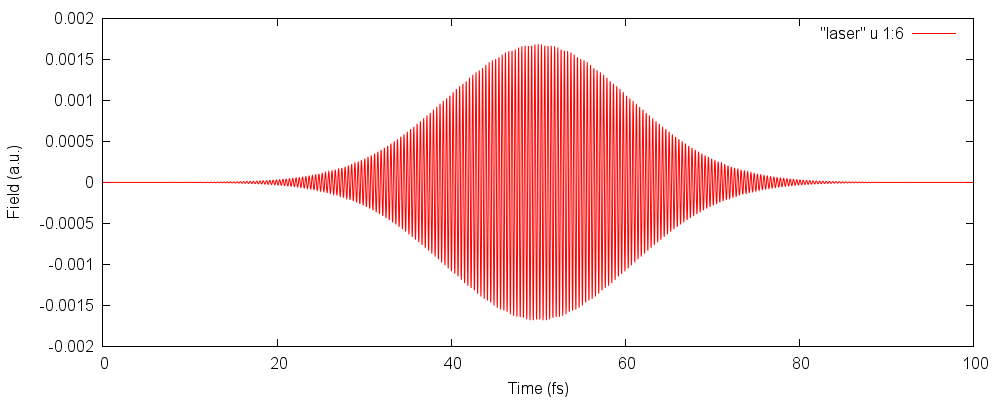
\includegraphics[width=0.75\textwidth]{figures/laser.png}
  \caption{Plot of the $z$ component of the generated laser field.}
  \label{fig:laser}
\end{figure}


% ======================================================================================================
% ======================================================================================================
% ======================================================================================================

\chapter{Usage of the Interfaces}
\refermanual{m-sec:int:overview}

Within \sharc, the quantum chemistry calculations are always performed by the quantum chemistry interfaces, which provide a unified way to carry out the quantum chemistry independent of the used program.
Hence, in principal every part of \sharc\ is compatible with the different quantum chemistry programs (with some exceptions, e.g., \textsc{Gaussian} cannot provide spin-orbit couplings).
However, depending on the used program, some details---mostly related to preparation of the frequency calculation and of the template files---of the preparation steps change.
In the following, these details are addressed, in the order in which the interfaces are discussed in the Manual.

% ======================================================================================================

\section{\textsc{Molpro}}
\refermanual{m-sec:int:molpro}

The functionality of the \sharc-\textsc{Molpro} interface is very similar to the \sharc-\textsc{Molcas} interface.
Hence, users who went through the full tutorial in chapter \ref{chap:full} should feel familiar when using \textsc{Molpro} instead.

These are the main differences when using \textsc{Molpro} instead of \textsc{Molcas}:
\begin{itemize}
  \item \textsc{Molpro} calculations---single point, optimization, frequencies---can be setup with \ttt{molpro\_input.py}. This also allows preparing \textsc{Molden} files to be used with \ttt{wigner.py}.
  \item \ttt{molpro\_input.py} can write \ttt{MOLPRO.template} files. 
  \item \textsc{Molpro} can state-average over different multiplicities. Therefore, in \ttt{MOLPRO.template} one can define multiple independent CASSCF jobs, each with arbitrary state-averaging schemes. See the example files in \ttt{\$SHARC/../examples/SHARC\_MOLPRO/} for such a template file.
  \item \textsc{Molpro} can compute nonadiabatic coupling vectors. These can be used in \ttt{sharc.x} for electronic propagation and for the exact transformation of the gradient vectors. Related options can be set during the \ttt{setup\_traj.py} dialogue.
  \item Unlike the \textsc{Molcas} interface, the \textsc{Molpro} interface cannot perform CASPT2 or QM/MM calculations.
  \item Only segmented basis sets (e.g., Pople or Ahlrichs) can be used for the \sharc-\textsc{Molpro} interface, while generally contracted basis sets (e.g., Dunning or ANO) cannot be used because \textsc{Molpro} cannot calculate gradients with them.
  \item The \sharc-\textsc{Molpro} interface almost always requires \ttt{wfoverlap.x}, so this should be installed from the \link{https://sharc-md.org/?page_id=309}{\sharc\ homepage}.
  \item You can set \ttt{\$MOLPRO} to the main directory of \textsc{Molpro} in your Shell profile. \sharc\ scripts will generally notice that this variable is set, which will simplify the setup.
\end{itemize}

% ======================================================================================================

\section{\textsc{Molcas}}
\refermanual{m-sec:int:molcas}

\textsc{Molcas} is the program used in the full tutorial in Chapter~\ref{chap:full}.

% ======================================================================================================

\section{\textsc{Columbus}}
\refermanual{m-sec:int:columbus}

\textsc{Columbus} is a very complex suite of many independent programs, each with own input files which are strongly inter-dependent.
Hence, \sharc\ does not come with an input preparation tool like \ttt{molpro\_input.py} or \ttt{molcas\_input.py}.
Instead, users should use \textsc{Columbus}' interactive input facility, \ttt{colinp}.
Users who are new to \textsc{Columbus} should first work through the \link{http://www.univie.ac.at/columbus/docs_COL70/tutorial.pdf}{\textsc{Columbus} main tutorial} and the \link{http://www.univie.ac.at/columbus/docs_COL70/documentation_main.html}{\textsc{Columbus} online documentation} before starting to work with the \sharc-\textsc{Columbus} interface.

These are the main differences when using \textsc{Columbus} instead of \textsc{Molcas}:
\begin{itemize}
  \item Input preparation (both for regular \textsc{Columbus} calculations and for the interface template) is relatively complicated. See the following subsections for some general hints.
  \item \textsc{Columbus} has a number of hard internal limits: a maximum of 255 basis functions and a maximum of 65535 CSFs in MCSCF (CAS(16,12) or larger will not work).
  \item One can use either of two integral codes: \textsc{Dalton} or \textsc{Molcas}. The former can compute nonadiabatic coupling vectors, whereas the latter can compute spin-orbit couplings. For the latter, the \link{http://www.univie.ac.at/columbus/docs_COL70/columbus_molcas_link.html}{\textsc{Columbus-Molcas} interface} must be installed.
  \item One can use either of two CASSCF codes: \textsc{Columbus} own code or \textsc{Molcas} (faster, but no gradients). For the latter, the \link{http://www.univie.ac.at/columbus/docs_COL70/columbus_molcas_link.html}{\textsc{Columbus-Molcas} interface} must be installed.
  \item If planning to run CASSCF-based \sharc\ dynamics, we recommend to not use \textsc{Columbus}; instead, use \textsc{Molcas} or \textsc{Molpro}. \textsc{Columbus} should only be used for MRCI-based dynamics.
  \item MRCI-based dynamics can be very expensive. Careful setup is required.
  \item Running the \ttt{wfoverlap.x} program with MRCI wave functions can be quite expensive. Hence, users should carefully adjust the related wave function truncation threshold.
\end{itemize}






\subsection{General Hints for using \textsc{Columbus}}

In order to use \textsc{Columbus}, whether via its driver script \ttt{runc} or through the \sharc-\textsc{Columbus} interface, you have to set the environment variable \ttt{\$COLUMBUS} to the directory containing the \textsc{Columbus} executables (like \ttt{runc}, \ttt{mcscf.x}, \ttt{ciudg.x}, etc.).

In order to prepare a calculation, first convert the standard xyz file containing the molecular geometry to \textsc{Columbus} format:
\begin{verbatim}
user@host> $COLUMBUS/xyz2col.x < geom.xyz
\end{verbatim}
which will create the file \ttt{geom}. Then, start \ttt{colinp}
\begin{verbatim}
user@host> $COLUMBUS/colinp
\end{verbatim}

Go through the input sections, starting with the integral section, followed by SCF, CASSCF, MRCI and finally the run setup.
Advanced users can then manually alter the input files as necessary (e.g., to achieve a RAS-type reference wave function).
After the preparation of the input, start \textsc{Columbus} via
\begin{verbatim}
user@host> $COLUMBUS/runc -m [MEMORY in MB] > runls&
\end{verbatim}
An optimization can be carried out directly with \ttt{runc}---just use the corresponding options in \ttt{colinp}.

For a (numerical) frequency calculation, use \ttt{colinp} to generate the internal coordinates and the \ttt{DISPLACEMENT} directories. 
Then, a calculation needs to be carried out in each of the \ttt{DISPLACEMENT} subdirectories, a task which is accomplished by the \ttt{calc.pl} script, or by manually starting \ttt{runc} in each of the directories (this approach might be faster because the calculations can be parallelized). 
Subsequently, the script \ttt{forceconst.pl} can be used to collect the results, producing the file \ttt{suscalls} which is compatible with the \textsc{Molden} format (and can be used with \ttt{wigner.py}).

\subsection{COLUMBUS input for usage with the interface}

For the \sharc-\textsc{Columbus} interface, a template directory is needed.
The directory needs to contain one subdirectory with input for each ``job''.
Each job usually contains the input for one multiplicity; the exception is the computation of spin-orbit couplings, where several multiplicities are computed in the same job.
In order to prepare the input for the \sharc-\textsc{Columbus} interface with spin-orbit couplings, you can see the 
\link{http://www.univie.ac.at/columbus/docs_COL70/tutorial-SO.pdf}{tutorial on spin-orbit coupling calculations}.

\paragraph{Integral program input}

The interface is able to either use integrals from \textsc{Dalton} or from \textsc{Molcas}.
With \textsc{Dalton}, nonadiabatic coupling vectors can be computed but no spin-orbit couplings, with \textsc{Molcas} it is vice versa; hence, choose the integral program with care.

This is a step-by-step description for the integral setup:
\begin{enumerate}
  \item Run the preparation program (prepinp): yes
  \item Choose either \textsc{Dalton} or \textsc{Molcas}
  \item Choose the symmetry (input is different for \textsc{Dalton}---write \ttt{c1} for no symmetry---and \textsc{Molcas}---press \ttt{<ENTER>} for no symmetry)
  \item Provide the geometry file in \textsc{Columbus} format
  \item Provide the basis set
  \item For \textsc{Molcas}: include scalar relativity and spin-orbit integrals if desired
\end{enumerate}

\paragraph{SCF input}

Since the SCF step is actually not carried out if starting orbitals are provided, it is sufficient to setup a closed-shell neutral wave function with default parameters.

\paragraph{MCSCF input}

In the MCSCF section any desired state-averaging scheme can be defined. 

This is a step-by-step description for the MCSCF setup:
\begin{enumerate}
  \item Do not freeze any orbitals at the MCSCF level.
  \item If gradients are desired, always set up for CI gradients (even if doing MCSCF-level dynamics).
  \item Enter the number of distinct row tables (DRTs); you will need one DRT for each multiplicity included in the state-averaging.
  \item For each DRT, provide the MCSCF settings (number of electrons, multiplicity, symmetry (\ttt{1}), RAS settings (\ttt{0} and \ttt{0}).
  \item Provide the number of active orbitals, do not apply group restrictions.
  \item Set the convergence to very tight (this improves the computation of gradients), e.g., \ttt{knorm [1.e-6 ]  wnorm [1.e-6 ]  DE [1.e-10]}, and the number of states for state-averaging.
\end{enumerate}

\paragraph{CI input}

There are three possible ways to setup the CI input.
If you have only one multiplicity in this job, then use the \ttt{one-DRT case}.
If you have several multiplicities in this job but do not want to compute spin-orbit couplings, use \ttt{independent multiple-DRTs}.
If you have several multiplicities in this job and want to compute compute spin-orbit couplings, use the \ttt{one-DRT case}.

Make sure that all multiplicities used in the \sharc\ input are covered with all job directories.

This is a step-by-step description for the CI setup:
\begin{enumerate}
  \item Press \ttt{<ENTER>} to leave the DRT explanation text
  \item Choose \ttt{one-DRT case} or \ttt{independent multiple-DRTs} (as explained above)
  \item Choose \ttt{y} if you want to compute gradients
  \item If you want to compute spin-orbit couplings, enable \ttt{Spin-Orbit CI}, give the maximum multiplicity (e.g., \ttt{3}), and the spin representation (always \ttt{1 1 1})
  \item Complete the DRT input (number of electrons, symmetry (\ttt{1}), number of frozen core/virtual orbitals, internal orbitals, doubly-occupied, auxiliary, excitation level (CASSCF: \ttt{0}, MRCI: \ttt{1} or \ttt{2}), reference symmetry (\ttt{1}), no group restrictions)
  \item Choose \ttt{ciudg} (not \ttt{pciudg})
  \item Select \ttt{CI} as type of calculation
  \item Choose the number of roots (will be overridden by the interface, but choose at least \ttt{2} because the \ttt{colinp} sets up necessary input files) and \ttt{RTOL} for the CI procedure (\ttt{1e-4} or larger if performance is needed)
  \item Select at least one transition moment (will be overridden by the interface)
\end{enumerate}

\paragraph{Set up job control}

Most of the job control is overridden by the interface, but some options are needed to obtain all necessary input files.

This is a step-by-step description for the job setup:
\begin{enumerate}
  \item Choose \ttt{Job control for single point or gradient calculation}
  \item Choose \ttt{single point calculation}
  \item Select: \ttt{SCF}, \ttt{MCSCF}, \ttt{one-electron properties for all methods}, \ttt{transition moments for MR-CISD}, \ttt{nonadiabatic couplings (and/or gradients)}
  \item Also select either \ttt{MR-CISD (serial operation)} (no spin-orbit coupling) or \ttt{SO-CI coupled to non-rel. CI} (for spin-orbit coupling)
  \item If \ttt{SO-CI coupled to non-rel. CI}, choose the number of states per multiplicity, e.g., \ttt{4:0:3} (will be overridden)
  \item Choose \ttt{first moments}
  \item Do not use \ttt{analysis in internal coordinates}
  \item Choose \ttt{DCI*(E2-E1) term (interstate coupling)} (or \ttt{DCI+DCSF term (non-adiabatic coupling)} when using \textsc{Dalton})
  \item Do not use \ttt{intersection analysis (slope)}
  \item Exit \ttt{colinp}
\end{enumerate}

Repeat these steps for all input directories if you have more than one job.





% ======================================================================================================

\section{Analytical expressions}
\refermanual{m-sec:int:analytical}

For the interface using analytical expressions for the potential energy surfaces, only one input file is needed (\ttt{Analytical.template}). This file contains the definitions of all analytical expressions. See below for an example of this file.

The remaining procedure with the analytical potential interface is analogous to the usage of the other interfaces.

\subsection{One-dimensional case}

In the following, we will prepare the input for a single particle moving in one dimension on two states.

The file \ttt{Analytical.template} consists of a file header and a file body. The header for the one-dimensional case and for two states could look as follows:
\begin{oframed}
\footnotesize\begin{Verbatim}[commandchars=\\\{\}]
1
2
H       x       0       0
\end{Verbatim}
\end{oframed}
The first line defines the number of atoms to be one, the second line gives the number of states. The third line is a mapping of the cartesian coordinates of the atom to variable names. In this case, the $x$ component of the coordinate of the atom is linked to the actual variable called \ttt{x}. The variable can then be used in the file body in the definitions of the potentials.

Below the file header (with $n_\text{atom}+2$ lines), different blocks can be put. Variable blocks define can be used to define constants:
\begin{oframed}
\footnotesize\begin{Verbatim}[commandchars=\\\{\}]
Variables
k 2.0
D12 10.0
Re 2.0
omega 13.
mu 1.0
End
\end{Verbatim}
\end{oframed}

Most importantly, matrix blocks define the potential energies, couplings and gradients. A matrix block could look like:
\begin{oframed}
\footnotesize\begin{Verbatim}[commandchars=\\\{\}]
Hamiltonian
0.5*k*x**2+omega,
0,   0.5*k*(x-Re)**2+D12,
\end{Verbatim}
\end{oframed}
Note the keyword \ttt{Hamiltonian}, which defines the type of matrix given.

Another matrix block gives the derivatives of the Hamiltonian with respect to the variable \ttt{x}:
\begin{oframed}
\footnotesize\begin{Verbatim}[commandchars=\\\{\}]
Derivatives     x
k*x,
0,   k*(x-Re),
\end{Verbatim}
\end{oframed}
The user has to provide the correct derivatives of the Hamiltonian manually.

Put together, the complete input for the example might look like:
\begin{oframed}
\footnotesize\begin{Verbatim}[commandchars=\\\{\}]
1
2
H       x       0       0

Variables
k 2.0
D12 10.0
Re 2.0
mu 1.0
End

Hamiltonian
0.5*k*x**2,
0,   0.5*k*(x-Re)**2+D12,

Derivatives     x       \textcolor{blue}{# Derivatives with respect to x}
k*x,                    \textcolor{blue}{# Derivatives need to be given manually}
0,   k*(x-Re),

Dipole  1
0.0,
0.5*mu, 0.0,

\end{Verbatim}
\end{oframed}

Only the \ttt{Hamiltonian} block and one \ttt{Derivatives} block for each variable needs to be present. Optional blocks are \ttt{SpinOrbit}, \ttt{Dipole} and \ttt{Dipolederivaties}. 

For more details please refer to the manual.




% ======================================================================================================

\section{ADF}
\refermanual{m-sec:int:adf}

Using ADF in combination with \sharc\ is slightly different from the multi-reference programs explained above, mostly because TD-DFT is a single-reference method.
This means that TD-DFT is comparably easy to use---there is no active space and no state-averaging (so adding more states to the computation does not affect the lower states).
On the contrary, TD-DFT will often fail to converge when the energy gap between the ground state and the excited state becomes small.
Another difference is that the ground state and the excited states are not treated equally---excited-state gradients are more expensive than the ground state gradient, and no transition dipole moments between two excited states can be computed.
Yet another important difference is that spin-orbit couplings can only be computed between singlets and triplets (unlike in the multi-reference codes, where all multiplicities can be used).

These are the main differences when using ADF instead of \textsc{Molcas}:
\begin{itemize}
  \item ADF calculations---single points, optimizations, frequency calculations---can be setup with ADF's suite of GUI programs, or with\sharc's \ttt{ADF\_input.py}.
  \item The result of ADF frequency calculations (standard output or \ttt{TAPE21}) can be converted to \textsc{Molden} format using \ttt{ADF\_freq.py}.
  \item Before starting ADF or any Python script related to ADF, source the relevant \ttt{adfrc.sh} file which came with ADF.
  \item Template files for the \sharc-ADF interface should be created by copying and adjusting the documented example in \ttt{\$SHARC/../examples/SHARC\_ADF/}.
  \item ADF cannot compute nonadiabatic coupling vectors, so all \sharc-ADF simulations rely on \ttt{wfoverlap.x}.
  \item ADF can carry out QM/MM calculations, for which two extra input files need to be prepared (see manual).
\end{itemize}

For the reasons mentioned above, the dynamics of \ce{CH2NH2+} cannot be properly described with TD-DFT.
Users who intend to follow the tutorial with ADF instead of \textsc{Molcas} should therefore use a different molecule (\ce{SO2} might work well).

% ======================================================================================================

\section{\textsc{Turbomole}}
\refermanual{m-sec:int:ricc2}

The \sharc-\textsc{Turbomole} interface can carry out ADC(2) and CC2 calculations.
Note that the interface does not allow using \textsc{Turbomole}'s TD-DFT functionality (for TD-DFT, one can use ADF or \textsc{Gaussian} instead).
ADC(2) and CC2 are single-reference methods.
This means that they are comparably easy to use---there is no active space and no state-averaging (so adding more states to the computation does not affect the lower states).
On the contrary, ADC(2) and CC2 will often fail to converge when the energy gap between the ground state and the excited state becomes small.
Another difference is that the ground state and the excited states are not treated equally---excited-state gradients are more expensive than the ground state gradient, and no transition dipole moments between two excited states can be computed.
Yet another important difference is that the \sharc-\textsc{Turbomole} interface can only deal with singlets and triplets currently.

Also note that within \sharc, spin-orbit couplings are only available with ADC(2), but not with CC2.

These are the main differences when using ADC(2) in \textsc{Turbomole} instead of \textsc{Molcas}:
\begin{itemize}
  \item \textsc{Turbomole} calculations---single points, optimizations, frequency calculations---can be setup with \textsc{Turbomole}'s input facility \ttt{define}.
  \item (For MP2 frequencies with \ttt{ricc2}, use \ttt{NumForce -ri -level mp2}, instead of the \ttt{NumForce -level CC2} claimed in the \textsc{Turbomole} documentation.)
  \item The result of \textsc{Turbomole} frequency calculations can be converted to \textsc{Molden} format using \textsc{Turbomole}'s \ttt{tm2molden} program.
  \item Template files for the \sharc-\textsc{Turbomole} interface should be created by copying and adjusting the documented example in \ttt{\$SHARC/../examples/SHARC\_RICC2/}.
  \item \textsc{Turbomole} cannot compute nonadiabatic coupling vectors, so all \sharc-\textsc{Turbomole} simulations rely on \ttt{wfoverlap.x}.
  \item You can set \ttt{\$TURBODIR} to the main path of \textsc{Turbomole} in your Shell profile. \sharc\ scripts will recognize this variable, which will simplify the setup.
\end{itemize}

% ======================================================================================================

\section{LVC Models}
\refermanual{m-sec:int:lvc}
\refermanual{m-sec:setup_LVCparam.py}

The linear-vibronic coupling model interface uses analytical expressions (like the analytical interface).
However, the LVC interface allows more complicated, realistic models for many-atom molecules, which can be automatically parametrized from a single point calculation.

In the following, a brief tutorial is given how to prepare the template file for the LVC interface for \ce{SO2} (this molecule should work well for LVC simulations) with the help of \textsc{Molpro}.
\begin{enumerate}
  \item Perform a frequency calculation for \ce{SO2}, e.g., using MP2 (setup can be done with \ttt{molpro\_input.py}).
  \item Run \ttt{python \$SHARC/wigner.py -l freq.molden}. This creates a file called \ttt{V0.txt}.
  \item In order to carry out the required single point calculation:
  \begin{enumerate}
    \item Use \ttt{wigner.py} to create a \ttt{initconds} file.
    \item Use \ttt{molpro\_input.py} to create a template file (use a segmented basis like \ttt{def2-SVP}).
    \item Use \ttt{setup\_init.py} to create a single point calculation at the equilibrium geometry in \ttt{ICOND\_00000/}.
    \item In \ttt{ICOND\_00000/QM.in}, add the keywords \ttt{grad} and \ttt{nacdr}. 
    \item Run the computation in \ttt{ICOND\_00000/}.
  \end{enumerate}
  \item Copy \ttt{V0.txt} and \ttt{ICOND\_00000/QM.out} to the same directory and execute \ttt{QMout2LVC.py} there.
\end{enumerate}
This creates the file \ttt{LVC.template}, which can be used as any other template file within \sharc.

Note that this mini-tutorial cannot be done with \textsc{Molcas}, because it does not return all $3N$ normal modes in its \textsc{Molden} files (only $3N-6$).
Among the \sharc\ interfaces, only the \textsc{Columbus} interface and the \textsc{Molpro} interface can be used to compute nonadiabatic coupling vectors and deliver the full $3N$ normal modes.
However, in systems where nonadiabatic couplings are not relevant (e.g., only one singlet and one triplet, or systems where the nonadiabatic couplings at the equilibrium geometry vanish by symmetry) all interfaces can be used for generating the \ttt{LVC.template} (in this case, do not add the \ttt{nacdr} keyword to \ttt{QM.in}).

% ======================================================================================================

\section{\textsc{Gaussian}}
\refermanual{m-sec:int:gaussian}

Using \textsc{Gaussian} in combination with \sharc\ is slightly different from the multi-reference programs explained above, mostly because TD-DFT is a single-reference method.
This means that TD-DFT is comparably easy to use---there is no active space and no state-averaging (so adding more states to the computation does not affect the lower states).
On the contrary, TD-DFT will often fail to converge when the energy gap between the ground state and the excited state becomes small.
Another difference is that the ground state and the excited states are not treated equally---excited-state gradients are more expensive than the ground state gradient, and no transition dipole moments between two excited states can be computed.
Yet another important difference is that spin-orbit couplings can not be computed with the \sharc-\textsc{Gaussian} interface currently.

These are the main differences when using \textsc{Gaussian} instead of \textsc{Molcas}:
\begin{itemize}
  \item \textsc{Gaussian} calculations---single points, optimizations, frequency calculations---can be setup with \textsc{Gaussian}'s GUI program, \ttt{gaussview}, or manually.
  \item In order to convert the result of a \textsc{Gaussian} frequency calculations to \textsc{Molden} format, load the standard output file into \textsc{Molden} and save in \textsc{Molden} format.
  \item Template files for the \sharc-\textsc{Gaussian} interface should be created by copying and adjusting the documented example in \ttt{\$SHARC/../examples/SHARC\_GAUSSIAN/}.
  \item \textsc{Gaussian} cannot compute nonadiabatic coupling vectors, so all \sharc-\textsc{Gaussian} simulations rely on \ttt{wfoverlap.x}.
  \item The \sharc-\textsc{Gaussian} interface currently cannot carry out QM/MM calculations.
\end{itemize}

For the reasons mentioned above, the dynamics of \ce{CH2NH2+} cannot be properly described with TD-DFT.
Users who intend to follow the tutorial with \textsc{Gaussian} instead of \textsc{Molcas} should therefore use a different molecule (\ce{SO2} might work well).

% ======================================================================================================

\section{\textsc{Orca}}
\refermanual{m-sec:int:orca}

Using \textsc{Orca} in combination with \sharc\ is slightly different from the multi-reference programs explained above, mostly because TD-DFT is a single-reference method.
This means that TD-DFT is comparably easy to use---there is no active space and no state-averaging (so adding more states to the computation does not affect the lower states).
On the contrary, TD-DFT will often fail to converge when the energy gap between the ground state and the excited state becomes small.
Another difference is that the ground state and the excited states are not treated equally---excited-state gradients are more expensive than the ground state gradient, and no transition dipole moments between two excited states can be computed.

These are the main differences when using \textsc{Orca} instead of \textsc{Molcas}:
\begin{itemize}
  \item \textsc{Orca} calculations---single points, optimizations, frequency calculations---can be setup with different GUI programs, e.g., \ttt{Gabedit}, or manually.
  \item The result of \textsc{Orca} frequency calculations (standard output) can be converted to \textsc{Molden} format using \ttt{Orca\_freq.py}.
  \item Template files for the \sharc-\textsc{Orca} interface should be created by copying and adjusting the documented example in \ttt{\$SHARC/../examples/SHARC\_ORCA/}.
  \item \textsc{Orca} cannot compute nonadiabatic coupling vectors, so all \sharc-\textsc{Orca} simulations rely on \ttt{wfoverlap.x}.
  \item The \sharc-\textsc{Orca} interface can carry out QM/MM calculations, with the MM part being computed in \textsc{Tinker}.
\end{itemize}

For the reasons mentioned above, the dynamics of \ce{CH2NH2+} cannot be properly described with TD-DFT.
Users who intend to follow the tutorial with \textsc{Orca} instead of \textsc{Molcas} should therefore use a different molecule (\ce{SO2} might work well).




% ======================================================================================================
% ======================================================================================================
% ======================================================================================================

\chapter{Quick Tutorial}

This quick tutorial presents how to setup a single \sharc\ trajectory, by simply creating all necessary input files without employing the tools of the \sharc\ suite.
In this quick tutorial, we are using the equilibrium geometry as starting geometry and random initial velocities. 

The goal is to prepare all input files for \sharc\ and the \textsc{Molcas} interface. 
The necessary files and directories are presented in figure~\ref{fig:traj_dir}. 
Note that the files \ttt{MOLCAS.template} and \ttt{MOLCAS.resources} are only necessary since we are using the \sharc-\textsc{Molcas} interface.

\begin{figure}
  \centering
  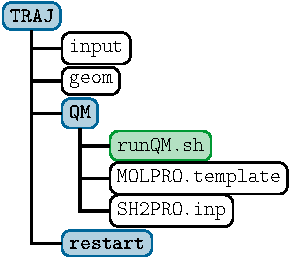
\includegraphics[]{img/dir_traj/dir_traj.pdf}
  \caption{Input files for a \sharc\ dynamics simulation of a single, independent trajectory.}
  \label{fig:traj_dir}
\end{figure}

The contents of the files are given and explained in the following.
Please be aware that the two subdirectories need to exist before \sharc\ can be started.

\section{Input File}

The \sharc\ input file (``\ttt{input}'') contains the dynamics settings and names of additional input files (geometry, velocity, coefficients). An example is given below:
\definecolor{shadecolor}{HTML}{BBDDFF}
\begin{example}\vspace{-8mm}
\begin{verbatim}
geomfile "geom"
veloc random 0.1

nstates 4 0 3
state 3 mch
coeff auto

ezero -94.41294549
tmax 25.000000
stepsize 0.5

surf sharc
coupling overlap
decoherence_scheme edc

grad_select
eselect 0.1
select_directly
\end{verbatim}\vspace{-5mm}
\end{example}

The meaning of these keywords is: The geometry is read from file \ttt{geom}. 
The nuclear velocities are picked at random, with 0.1~eV kinetic energy per atom. 
Four singlet states and three triplet states will be included in the simulation (0 is the number of doublet states). 
The initial state is the third state (the $S_2$). 
The initial coefficients will be set automatically (the initial state will have a coefficient of 1.0, the remaining states a coefficient of zero). 
The diagonal elements of the Hamiltonian will be shifted by $-94.41294549$~Hartree. 
The simulation will run for 25~fs with a 0.5 fs timestep. 
The \sharc\ formalism will be used (propagation on the diagonalized states). 
Nonadiabatic interactions are described with wavefunction overlaps.
SHARC will select which gradients to compute at each time step, with a selection threshold of 0.1~eV.
SHARC will select these gradients directly, without doing two quantum chemistry calculations per time step.

\section{Geometry File}

The geometry file ``\ttt{geom}'' contains the chemical symbols, atomic charge, $x$, $y$ and $z$ coordinates and the relative atomic masses.

\definecolor{shadecolor}{HTML}{BBDDFF}
\begin{example}\vspace{-8mm}
\begin{verbatim}
C 6.0 +0.00000000 +0.00000000 +0.00000000 12.00000000
N 7.0 +0.00000000 +0.00000000 +2.45664494 14.00307401
H 1.0 +1.78220520 +0.00000000 -1.02895628 1.00782504
H 1.0 +1.78220520 +0.00000000 +3.55174167 1.00782504
H 1.0 -1.78220520 +0.00000000 +3.55174167 1.00782504
H 1.0 -1.78220520 +0.00000000 -1.02895628 1.00782504
\end{verbatim}\vspace{-5mm}
\end{example}

\section{QM Run Script}

At each timestep, \sharc\ writes the current geometry and different keywords to the file \ttt{QM/QM.in} and then calls \ttt{runQM.sh}. 
After this call is finished, \sharc\ reads the results of the quantum chemistry calculation from \ttt{QM.out}.

In most of the cases, in \ttt{runQM.sh} simply one of the \sharc-interfaces is called:
\definecolor{shadecolor}{HTML}{BBDDFF}
\begin{example}\vspace{-8mm}
\begin{verbatim}
cd QM
$SHARC/SHARC_MOLCAS.py QM.in >> QM.log 2>> QM.err
\end{verbatim}\vspace{-5mm}
\end{example}
The interface will do all work necessary to produce the desired file \ttt{QM.out}.

\section{MOLCAS Template}

The \textsc{Molcas} interface needs as additional input file giving the settings for the electronic structure calculation. 
The file is called ``\ttt{MOLCAS.template}''.
It employs a simple keyword-argument structure and looks like:
\definecolor{shadecolor}{HTML}{BBDDFF}
\begin{example}\vspace{-8mm}
\begin{verbatim}
basis cc-pVDZ
nactel 6
ras2 4
inactive 5
roots 4 0 3
method casscf
no-douglas-kroll
\end{verbatim}\vspace{-5mm}
\end{example}

\section{MOLCAS Resources}

The \textsc{Molcas} interface additionally needs some paths and resource settings, both of which are read from the file  ``\ttt{MOLCAS.resources}''.
\definecolor{shadecolor}{HTML}{BBDDFF}
\begin{example}\vspace{-8mm}
\begin{verbatim}
molcas /usr/license/molcas/molcas80
scratchdir $TMPDIR/WORK
savedir ../restart/

memory 1000
ncpu 1
\end{verbatim}\vspace{-5mm}
\end{example}

\section{Running \sharc}

With the input files prepared, the trajectory can then be started by simply executing:
\definecolor{shadecolor}{HTML}{BBDDFF}
\begin{example}\vspace{-8mm}
\begin{verbatim}
$SHARC/sharc.x input 
\end{verbatim}\vspace{-5mm}
\end{example}

\section{Output}

\sharc\ produces four output files, \ttt{output.log}, \ttt{output.lis}, \ttt{output.dat} and \ttt{output.xyz}. 
The file \ttt{output.log} contains mainly a listing of the chosen options and the resulting dynamics settings. 
At higher print levels, the log file contains also information per timestep. 
\ttt{output.lis} contains a table with one line per timestep, giving active states, energies and expectation values.
\ttt{output.dat} contains a list of all important matrices and vectors at each timestep. 
This information can be extracted with \ttt{data\_extractor.x} to yield plottable table files. 
\ttt{output.xyz} contains the geometries of all timesteps, allowing visualization of the trajectory with the appropriate software (e.g., \textsc{Molden}).












\end{document}
